% -*- coding: utf-8 -*-
% !TEX root = ../main.tex

\subsection{Cadre de lecture du run final}
\label{ssec:resultats_cadre}

Cette section rapporte les résultats du run final effectué avec la graine 42.
Le backbone W1 est commun à toutes les expériences : son objectif CBOW atteint
une loss de validation de $1{,}6634$. Cette valeur décrit la prédiction de
contexte de Word2Vec et ne doit pas être comparée directement à la binary
cross-entropy des classifieurs. La table d'embeddings utilisée à l'inférence
contient $100\,000$ paramètres. Les têtes H1/M1 et H2/M1 en contiennent
respectivement $104\,449$ et $234\,753$ : la tête représente ainsi $51{,}1\,\%$
du pipeline H1 et $70{,}1\,\%$ du pipeline H2 avant pruning.

Les figures sont séparées selon la nature des quantités représentées. Une
figure \emph{théorique} est calculée uniquement à partir des dimensions et des
masques. Une figure \emph{expérimentale} contient au moins une valeur observée :
loss, accuracy, F1, ROC-AUC, temps de scoring, latence ou taille sérialisée.
Cette convention est importante, car un poids mis à zéro demeure stocké et
calculé par une couche linéaire dense tant qu'aucun format sparse ou noyau
spécialisé n'est utilisé.

\subsection{Poids relatif de la tête et potentiel théorique}
\label{ssec:resultats_potentiel}

\begin{figure}[!htbp]
    \centering
    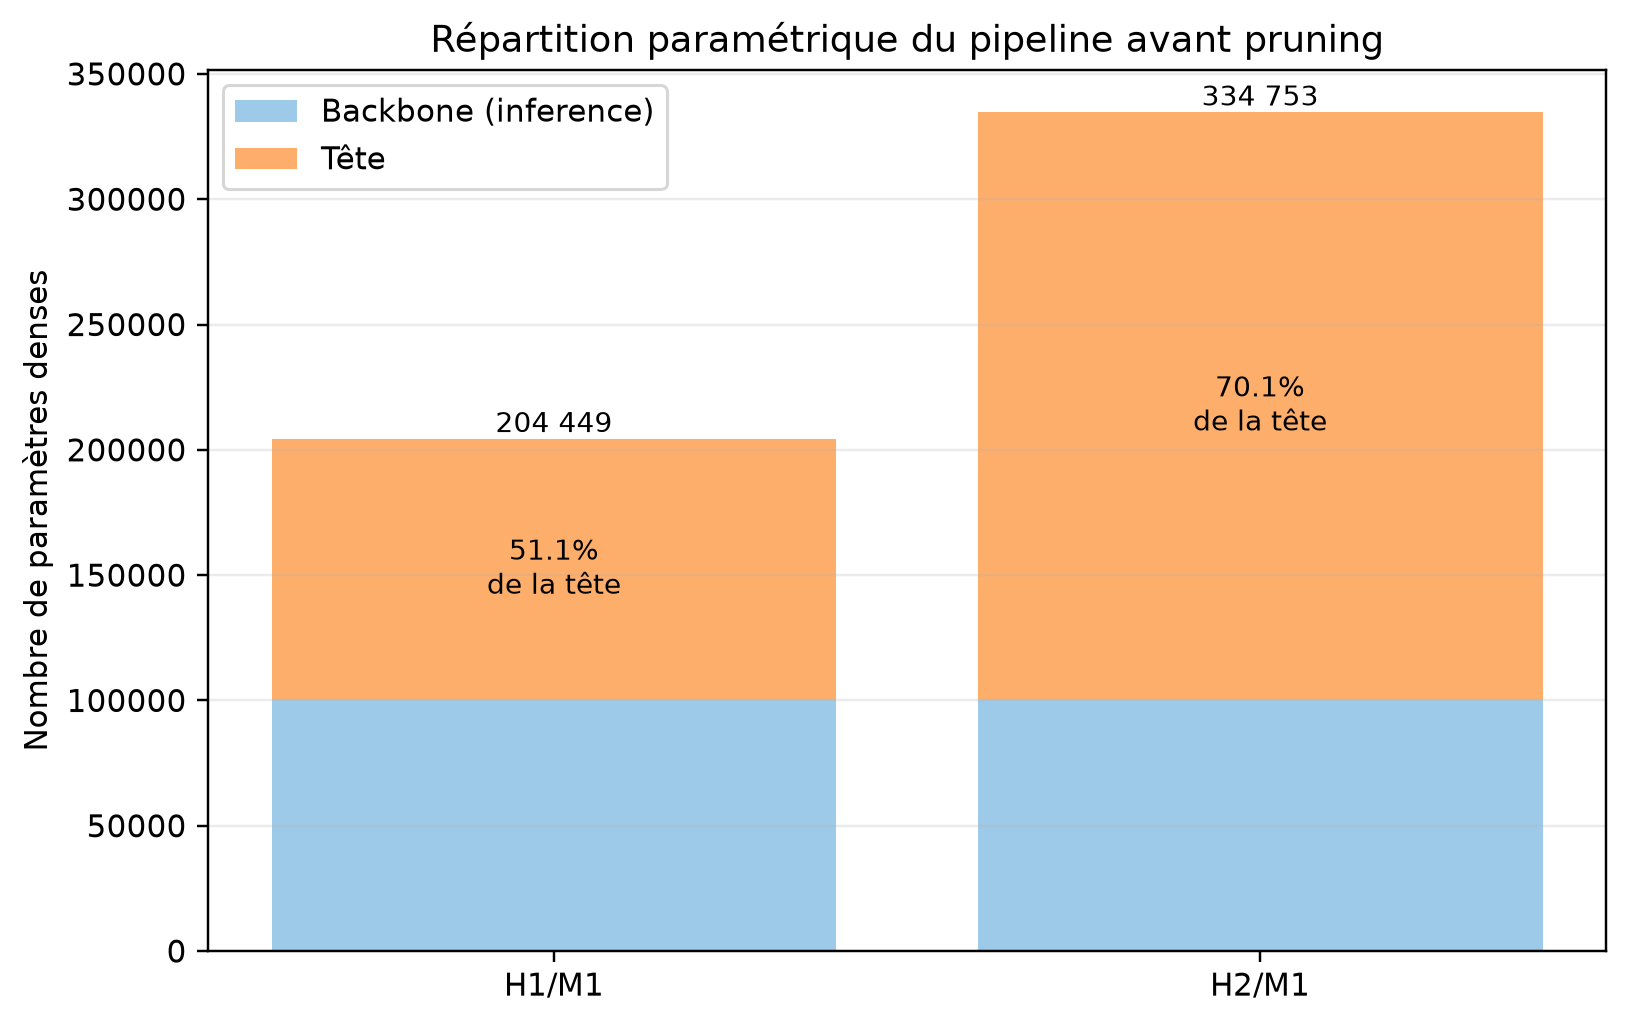
\includegraphics[width=0.82\textwidth]{../figures/theoriques/repartition_parametres_denses.png}
    \caption{Répartition des paramètres denses avant pruning. Le backbone ne
    compte ici que la table d'embeddings d'entrée nécessaire à l'inférence ; la
    table de sortie utilisée pour l'apprentissage CBOW est exclue. Le choix des
    nouvelles dimensions rend l'effet d'un pruning de la tête visible à
    l'échelle du pipeline complet.}
    \label{fig:resultats_repartition_parametres}
\end{figure}

La \autoref{fig:resultats_repartition_parametres} vérifie l'objectif recherché
par le changement d'hyperparamètres. Dans H1, le backbone et la tête ont des
tailles voisines ; dans H2, la tête contient plus de deux fois le nombre de
paramètres du backbone d'inférence. Une sparsification de H2 peut donc produire
un gain théorique sensible même lorsque W1 reste intact.

\begin{figure}[!htbp]
    \centering
    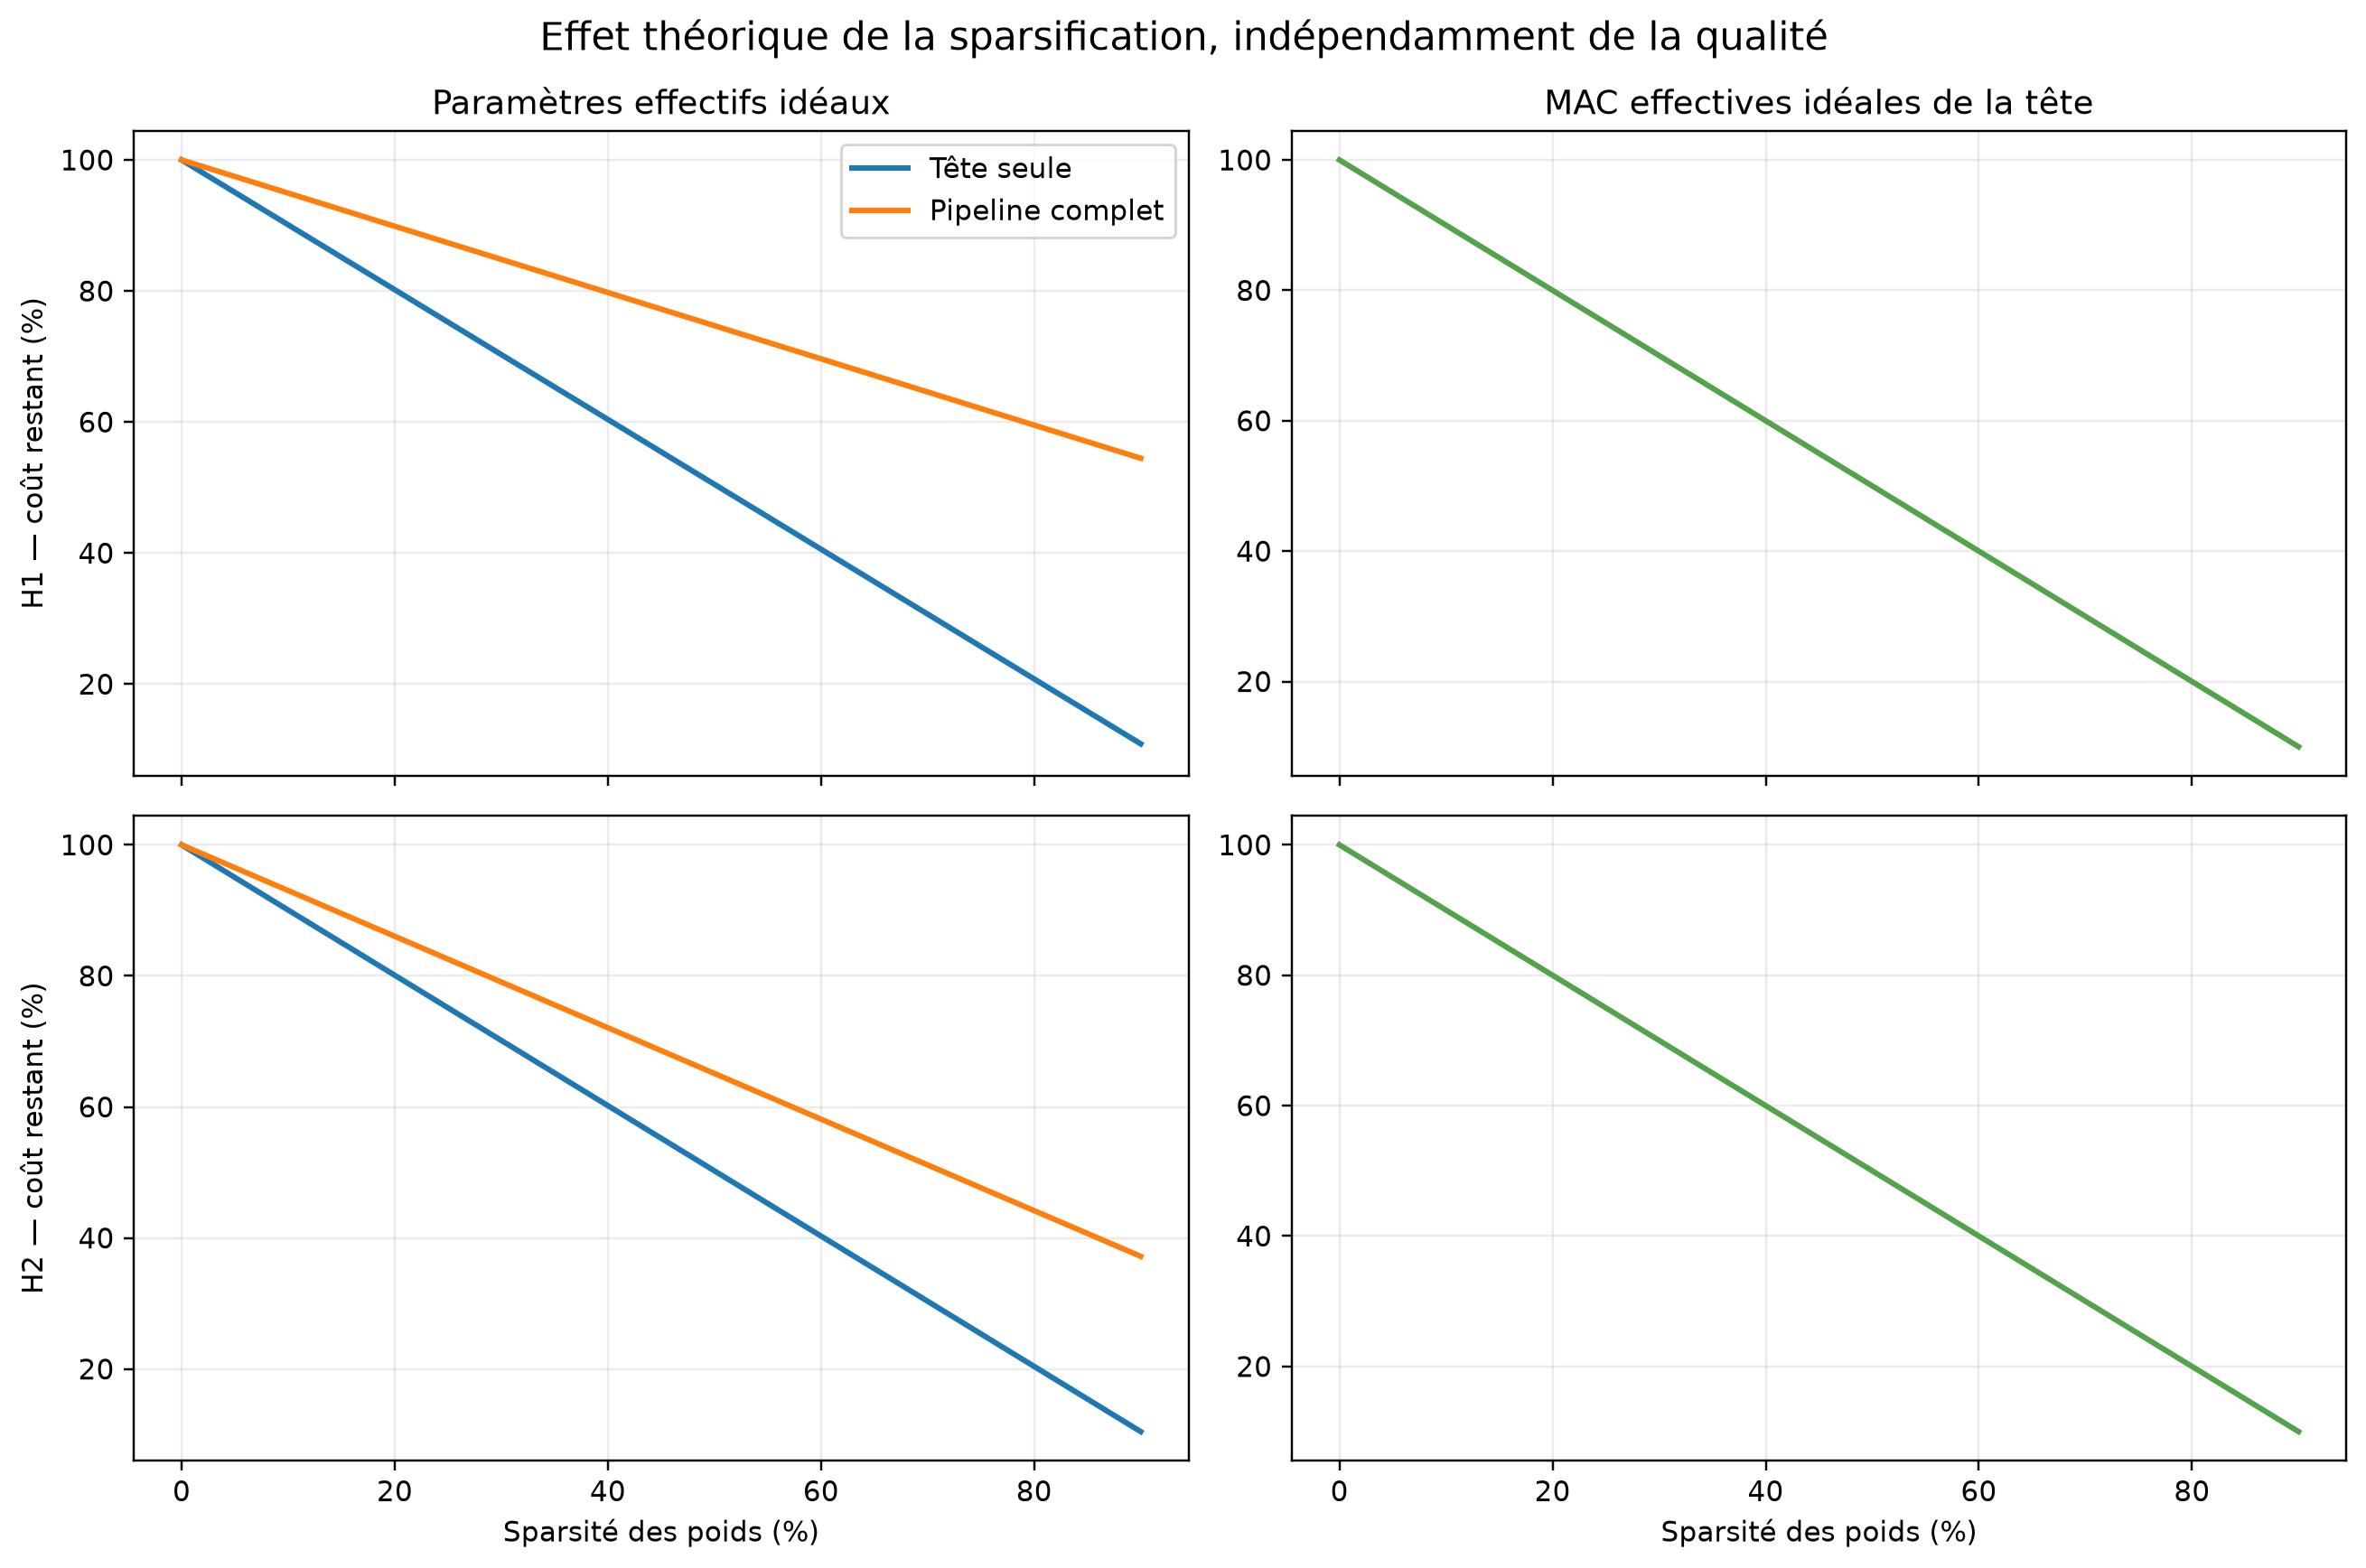
\includegraphics[width=0.94\textwidth]{../figures/theoriques/effet_theorique_sparsification.png}
    \caption{Effet théorique d'une sparsification croissante sur les paramètres
    et les MAC de la tête. Les coûts restants décroissent de façon affine avec
    la sparsité. Dans la vue des paramètres, la courbe du pipeline complet
    reste au-dessus de celle de la tête seule dès que la sparsité est non nulle,
    car elle inclut le coût fixe du backbone W1, qui n'est pas pruné. La
    réduction relative du pipeline est donc plus faible que celle de la tête.
    Ces courbes représentent un potentiel idéal, pas un gain matériel mesuré.}
    \label{fig:resultats_effet_theorique}
\end{figure}

À environ $50\,\%$ de sparsité, le nombre de paramètres effectifs de H1
passe de $104\,449$ à $52\,737$ et celui de H2 de $234\,753$ à environ
$118\,000$. En incluant W1, la réduction n'est plus de $50\,\%$, mais de
$25{,}3\,\%$ pour H1 et $34{,}9\,\%$ pour H2. Cette différence entre les deux
niveaux d'analyse justifie de les conserver dans toute la suite.

\subsection{Performances prédictives finales}
\label{ssec:resultats_tableau_principal}

Le \autoref{tab:resultats_principaux} rassemble les métriques du jeu de test.
Pour M2 et M3, la sparsité désigne la proportion de poids annulés dans la
tête. M4 est une architecture dense plus petite : sa sparsité interne vaut
donc zéro, même si son nombre de paramètres est voisin du nombre de paramètres
actifs des modèles prunés.

\begin{table}[!htbp]
    \centering
    \resizebox{\textwidth}{!}{%
    \begin{tabular}{|l|l|r|r|r|r|r|r|r|}
        \hline
        Tête & Modèle & Loss & Accuracy & F1 & ROC-AUC & Sparsité &
        $P_H^{\mathrm{eff}}$ & $P_{\mathrm{pipeline}}^{\mathrm{eff}}$ \\ \hline
        H1 & M1 & $0{,}5441$ & $72{,}92\,\%$ & $0{,}7397$ & $0{,}8009$ & $0\,\%$ & $104\,449$ & $204\,449$ \\ \hline
        H1 & M2 OBD & $0{,}5379$ & $73{,}20\,\%$ & $\mathbf{0{,}7561}$ & $0{,}8090$ & $50{,}00\,\%$ & $52\,737$ & $152\,737$ \\ \hline
        H1 & M3 OBD & $\mathbf{0{,}5353}$ & $\mathbf{73{,}57\,\%}$ & $0{,}7462$ & $\mathbf{0{,}8102}$ & $50{,}00\,\%$ & $52\,737$ & $152\,737$ \\ \hline
        H1 & M4 & $0{,}5449$ & $72{,}53\,\%$ & $0{,}7414$ & $0{,}7989$ & $0\,\%$ & $52\,225$ & $152\,225$ \\ \hline
        H2 & M1 & $\mathbf{0{,}5381}$ & $\mathbf{73{,}26\,\%}$ & $0{,}7393$ & $0{,}8038$ & $0\,\%$ & $234\,753$ & $334\,753$ \\ \hline
        H2 & M2 OBD & $0{,}5500$ & $72{,}07\,\%$ & $0{,}7441$ & $0{,}8027$ & $49{,}97\,\%$ & $118\,017$ & $218\,017$ \\ \hline
        H2 & M3 OBD & $0{,}5515$ & $73{,}02\,\%$ & $0{,}7435$ & $\mathbf{0{,}8048}$ & $49{,}97\,\%$ & $118\,017$ & $218\,017$ \\ \hline
        H2 & M4 & $0{,}5419$ & $72{,}92\,\%$ & $0{,}7449$ & $0{,}8029$ & $0\,\%$ & $117\,505$ & $217\,505$ \\ \hline
        H2 & MINT-M2 & $0{,}6787$ & $53{,}02\,\%$ & $0{,}2192$ & $0{,}7336$ & $49{,}95\,\%$ & $118\,063$ & $218\,063$ \\ \hline
        H2 & MINT-M3 & $0{,}5409$ & $72{,}68\,\%$ & $\mathbf{0{,}7505}$ & $0{,}8046$ & $49{,}95\,\%$ & $118\,063$ & $218\,063$ \\ \hline
    \end{tabular}}
    \caption{Résultats du run final sur les $3\,276$ textes de test. Les
    valeurs en gras indiquent le meilleur résultat de chaque tête et de chaque
    métrique ; elles ne constituent pas un test de significativité statistique.}
    \label{tab:resultats_principaux}
\end{table}

Pour H1, le pruning OBD ne dégrade pas la qualité : M2 obtient même le meilleur
F1 de la tête, $0{,}7561$, soit $+0{,}0165$ par rapport à M1. M3 présente la
meilleure loss, la meilleure accuracy et la meilleure ROC-AUC de H1, mais son
F1 est inférieur à celui de M2. Le réentraînement n'améliore donc pas toutes
les métriques simultanément. M4 reste proche de M1, ce qui indique qu'une tête
plus petite pouvait ici être entraînée directement sans perte importante.

L'absence de première place pour H1/M1 n'est pas paradoxale : une capacité plus
élevée ne garantit pas une meilleure généralisation. Surtout, ce classement ne
peut pas être attribué au seul pruning. OBD comporte six tours de trois
époques : M2 a déjà reçu 15 époques supplémentaires à partir du checkpoint M1,
et M3 en cumule 18. Comme M1 est sélectionné selon la loss de validation et que
le run n'utilise qu'une graine, le tableau montre que la compression préserve
la qualité, mais pas qu'elle améliore H1. Plusieurs graines et un protocole
d'entraînement strictement identique seraient nécessaires pour isoler cet effet.

Pour H2, les trois solutions de taille réduite après entraînement --- OBD-M2,
OBD-M3 et M4 --- atteignent des F1 compris entre $0{,}7435$ et $0{,}7449$. Le
meilleur F1 de H2 est obtenu par MINT-M3 avec $0{,}7505$, soit $+0{,}0112$ par
rapport à M1. Ce résultat doit toutefois être lu avec MINT-M2 : l'application
du masque seule fait chuter le F1 à $0{,}2192$. Sa précision reste élevée
($0{,}8963$), mais son rappel tombe à $0{,}1249$ ; le modèle prédit donc très
peu d'exemples positifs. Le réentraînement contraint est indispensable pour
recalibrer les activations et récupérer la performance.

\subsection{Convergence et comportement de la loss}
\label{ssec:resultats_convergence}

\begin{figure}[!htbp]
    \centering
    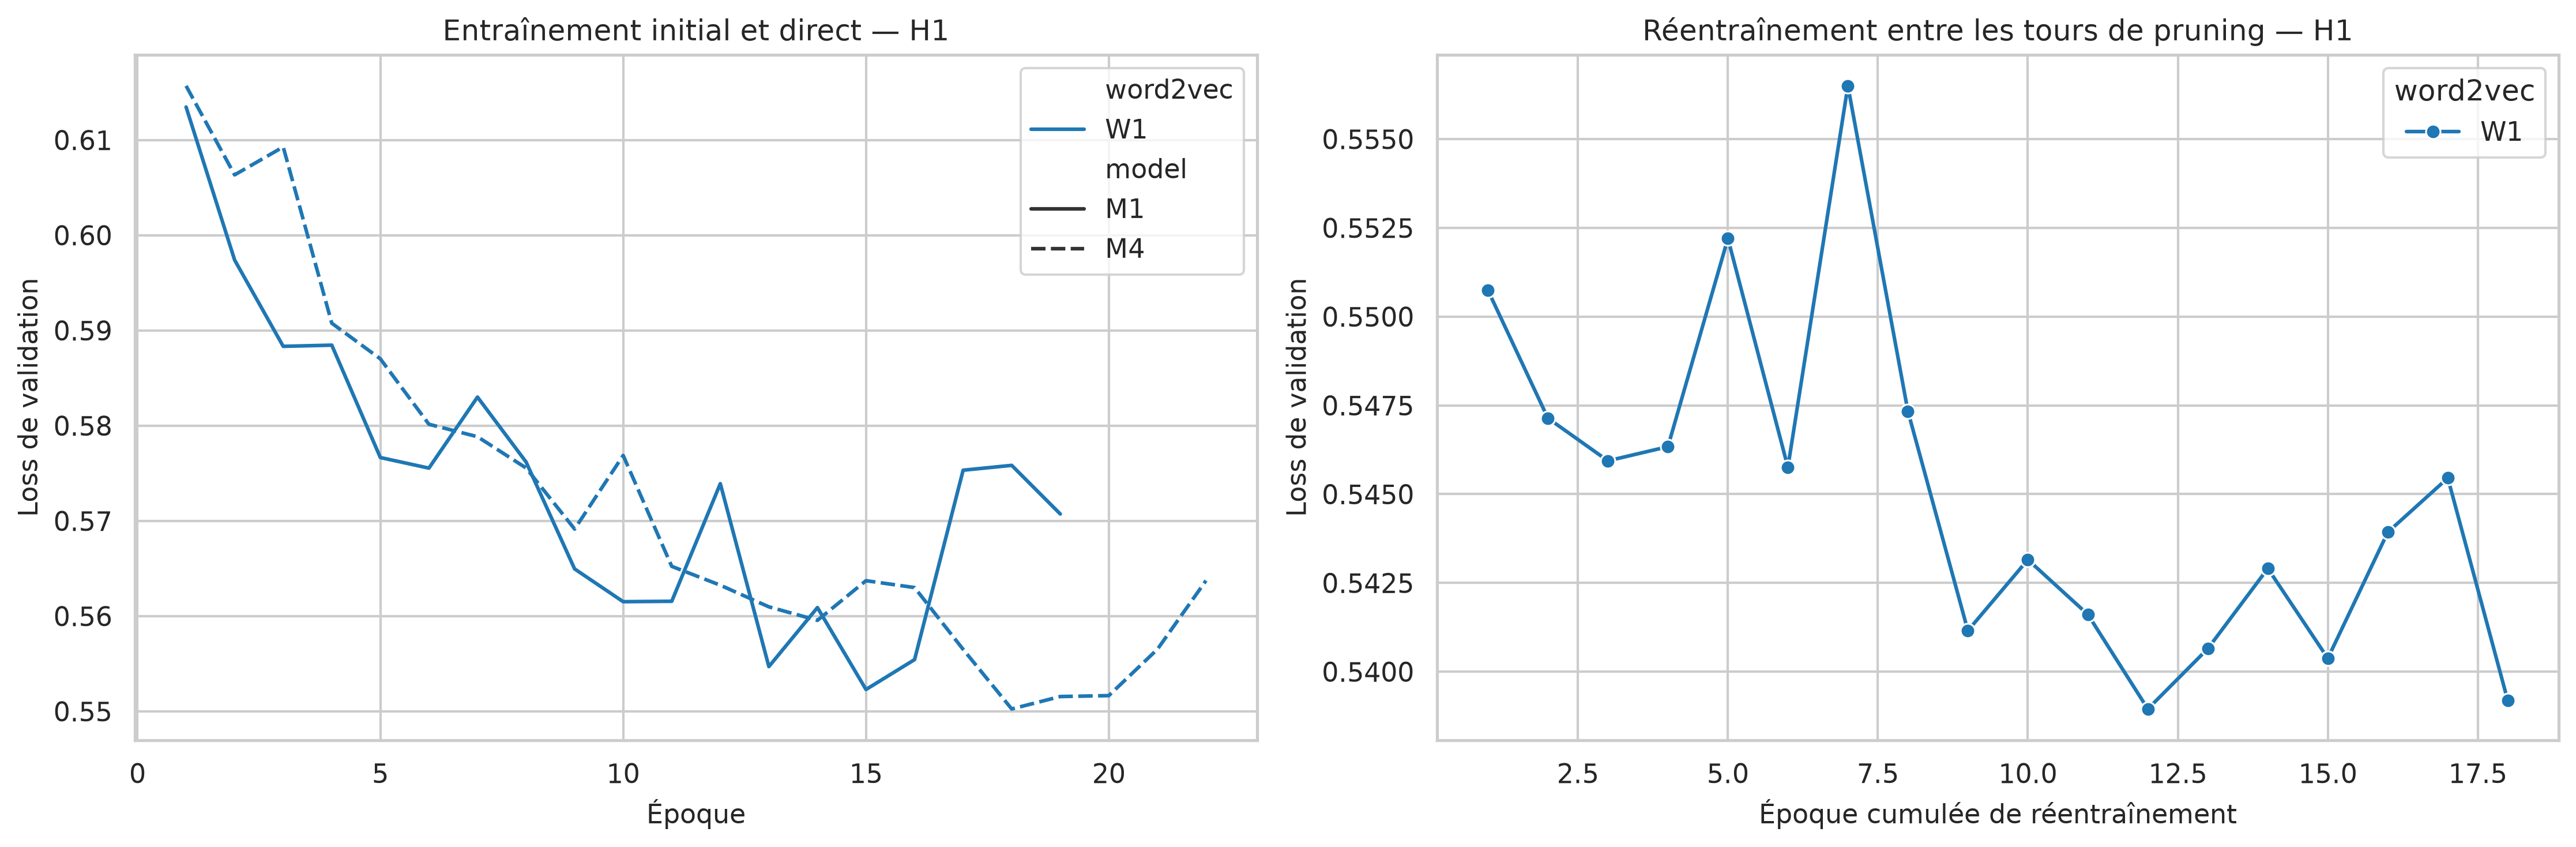
\includegraphics[width=0.94\textwidth]{../figures/experimentales/training_losses_H1.png}
    \par\smallskip\small (a) Tête H1.\par\medskip
    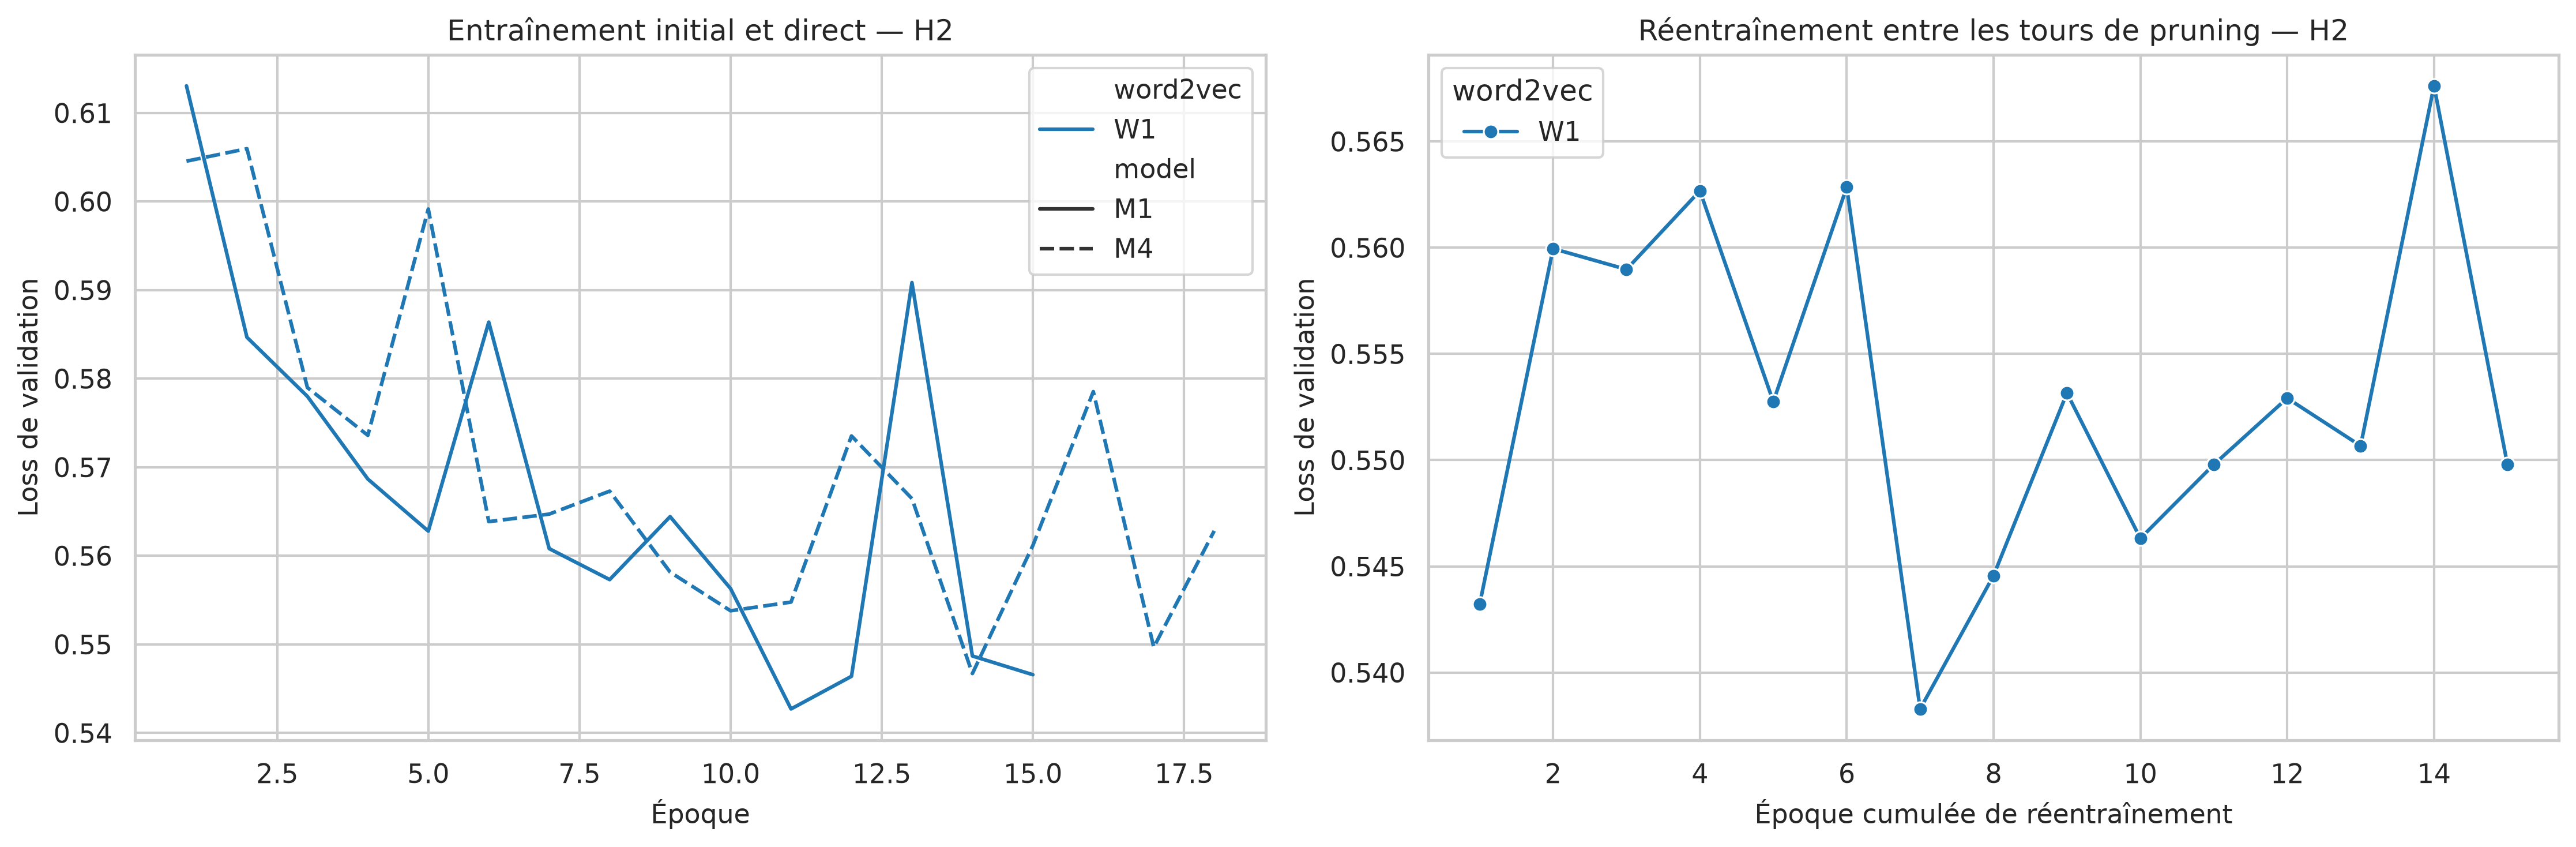
\includegraphics[width=0.94\textwidth]{../figures/experimentales/training_losses_H2.png}
    \par\smallskip\small (b) Tête H2.
    \caption{Loss de validation pendant l'entraînement dense de M1 et M4
    (graphiques de gauche) et pendant les réentraînements successifs d'OBD
    (graphiques de droite). L'abscisse des graphiques de droite concatène les
    trois époques de chaque tour de pruning.}
    \label{fig:resultats_training_losses}
\end{figure}

L'arrêt anticipé conserve l'époque de plus faible loss de validation. H1/M1
s'arrête après 19 époques et restaure l'époque 15
($\mathcal{L}_{\mathrm{val}}=0{,}5523$), tandis que H2/M1 s'arrête après 15
époques et restaure l'époque 11 ($0{,}5427$). Les oscillations visibles en
fin d'entraînement justifient ce mécanisme : la loss d'entraînement continue
de diminuer alors que la loss de validation ne s'améliore plus de manière
monotone. Les phases courtes de réentraînement OBD produisent elles aussi des
variations non monotones, ce qui explique qu'une amélioration de la loss ne se
traduise pas systématiquement par une hausse du F1 au seuil de décision $0{,}5$.

\subsection{Trajectoires du pruning OBD}
\label{ssec:resultats_obd}

\begin{figure}[!htbp]
    \centering
    \begin{minipage}[t]{0.49\textwidth}
        \centering
        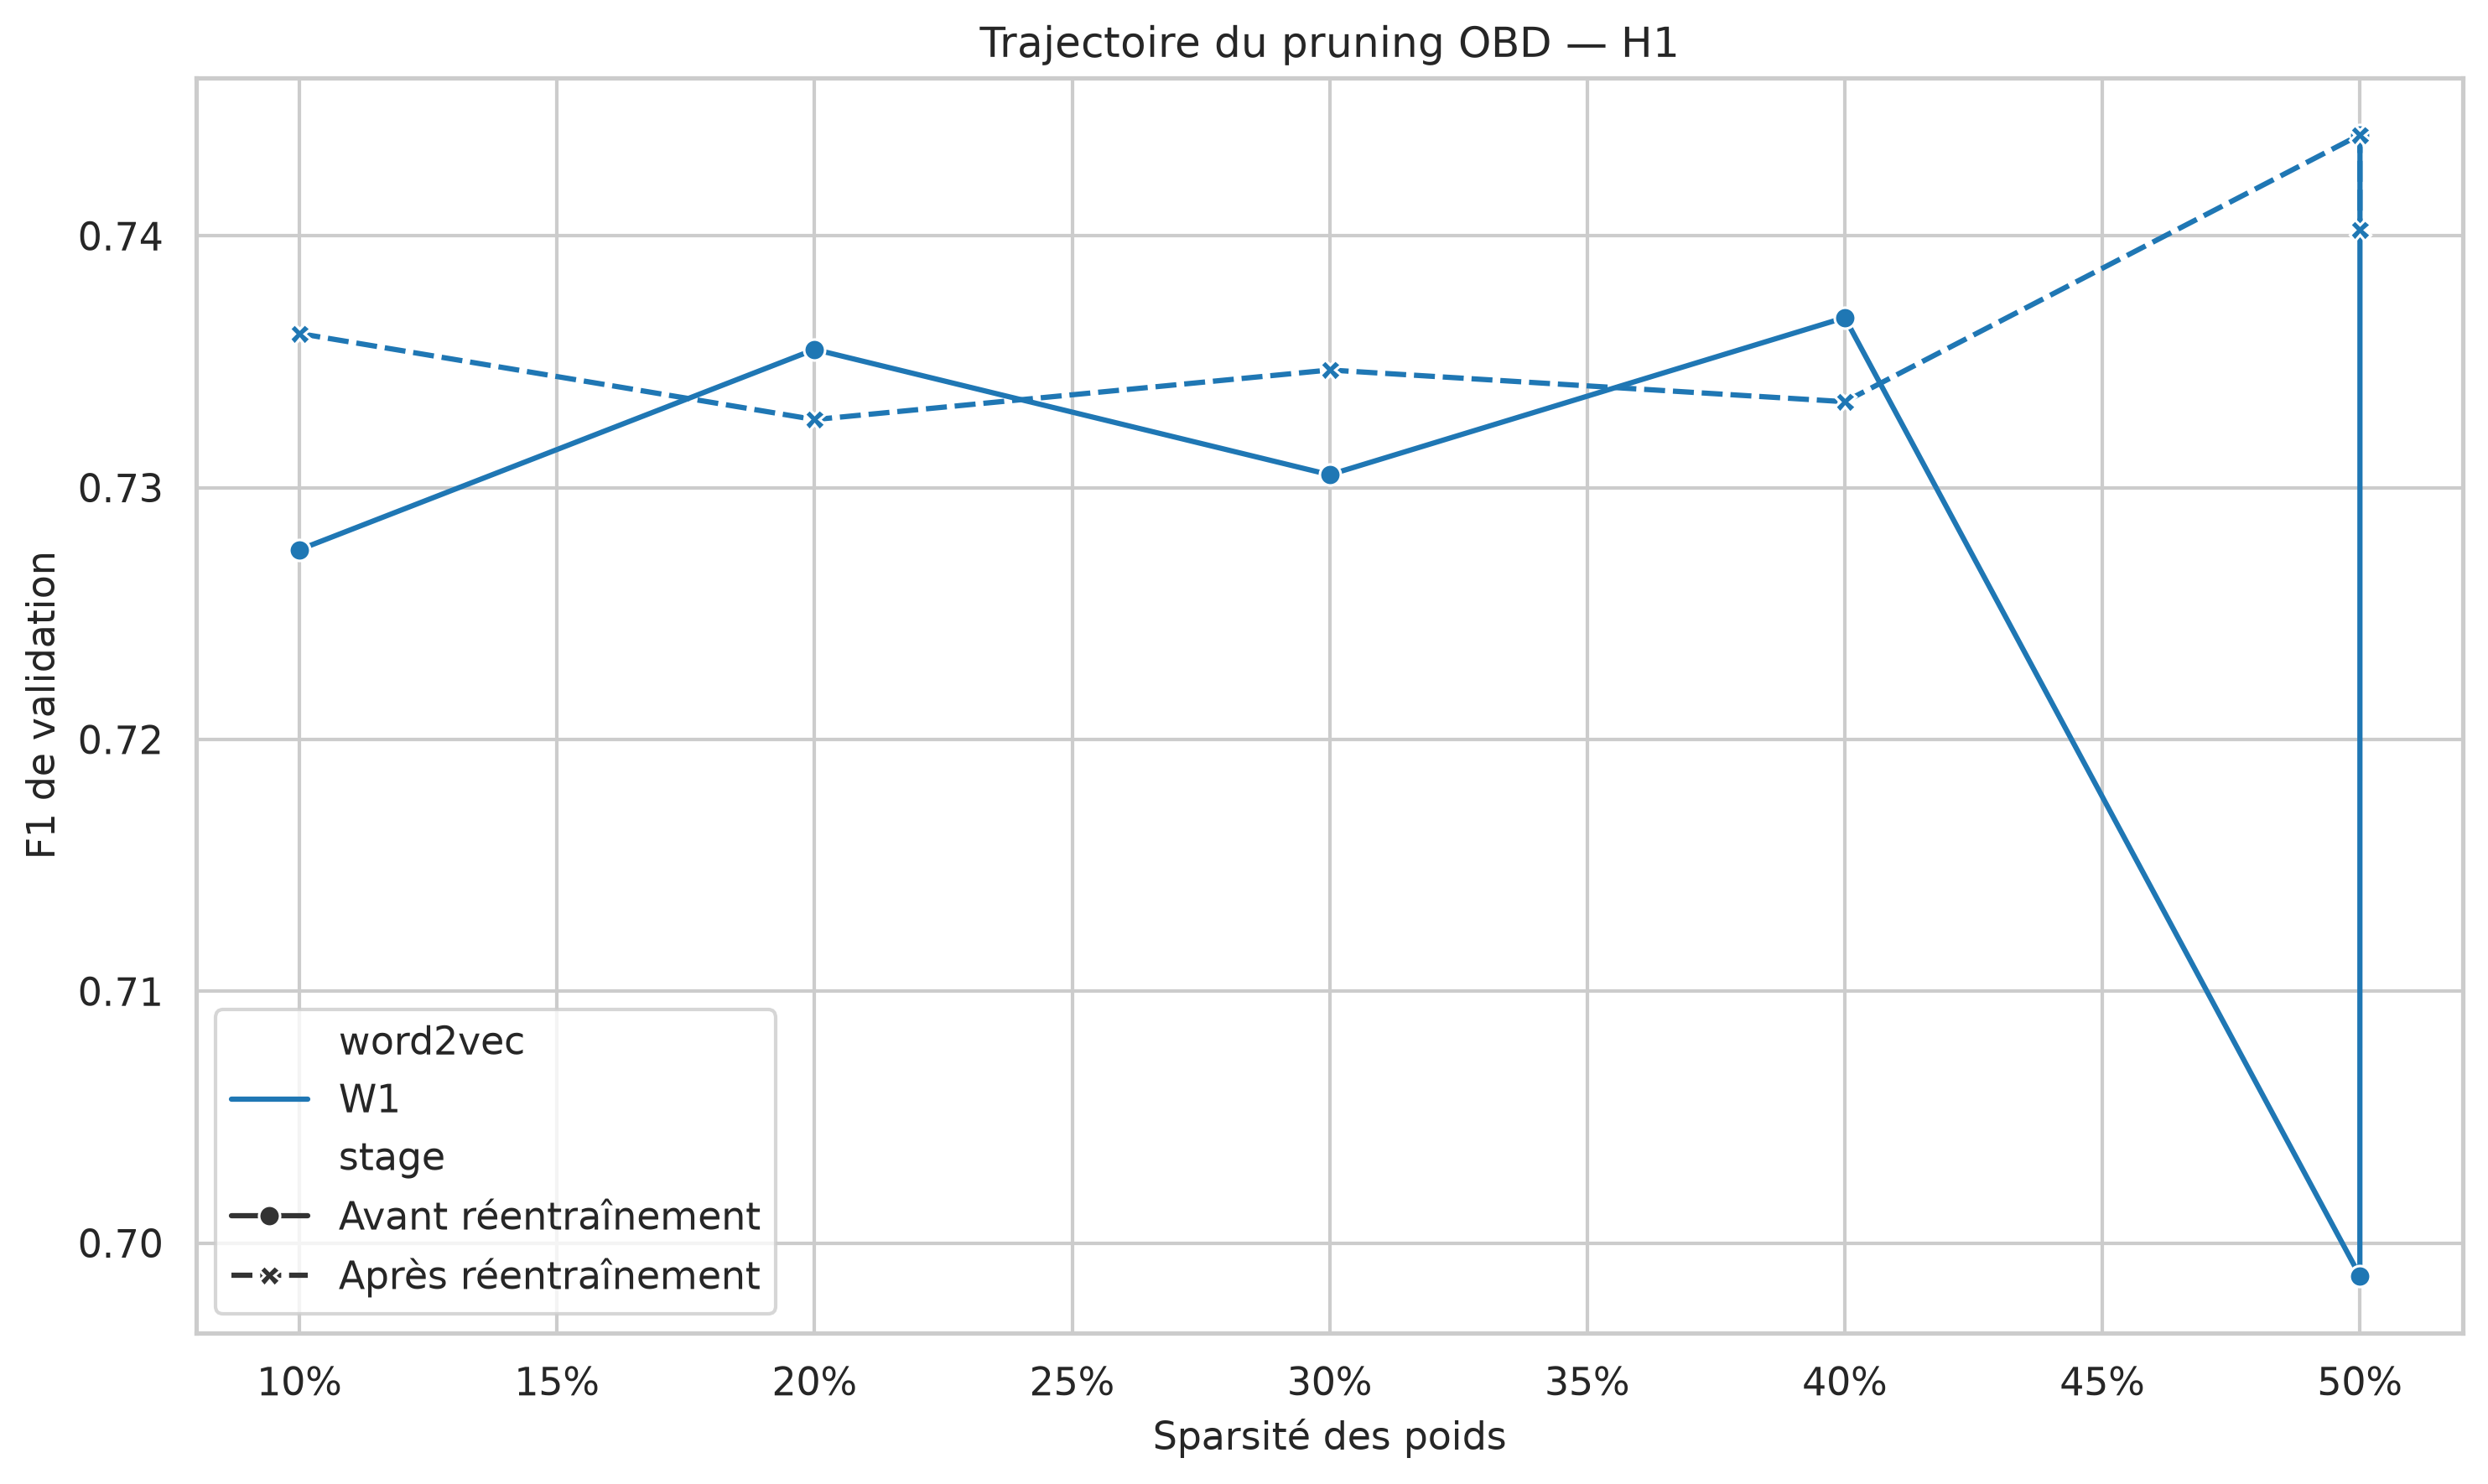
\includegraphics[width=\linewidth]{../figures/experimentales/pruning_trajectory_H1.png}
        \small (a) H1.
    \end{minipage}
    \hfill
    \begin{minipage}[t]{0.49\textwidth}
        \centering
        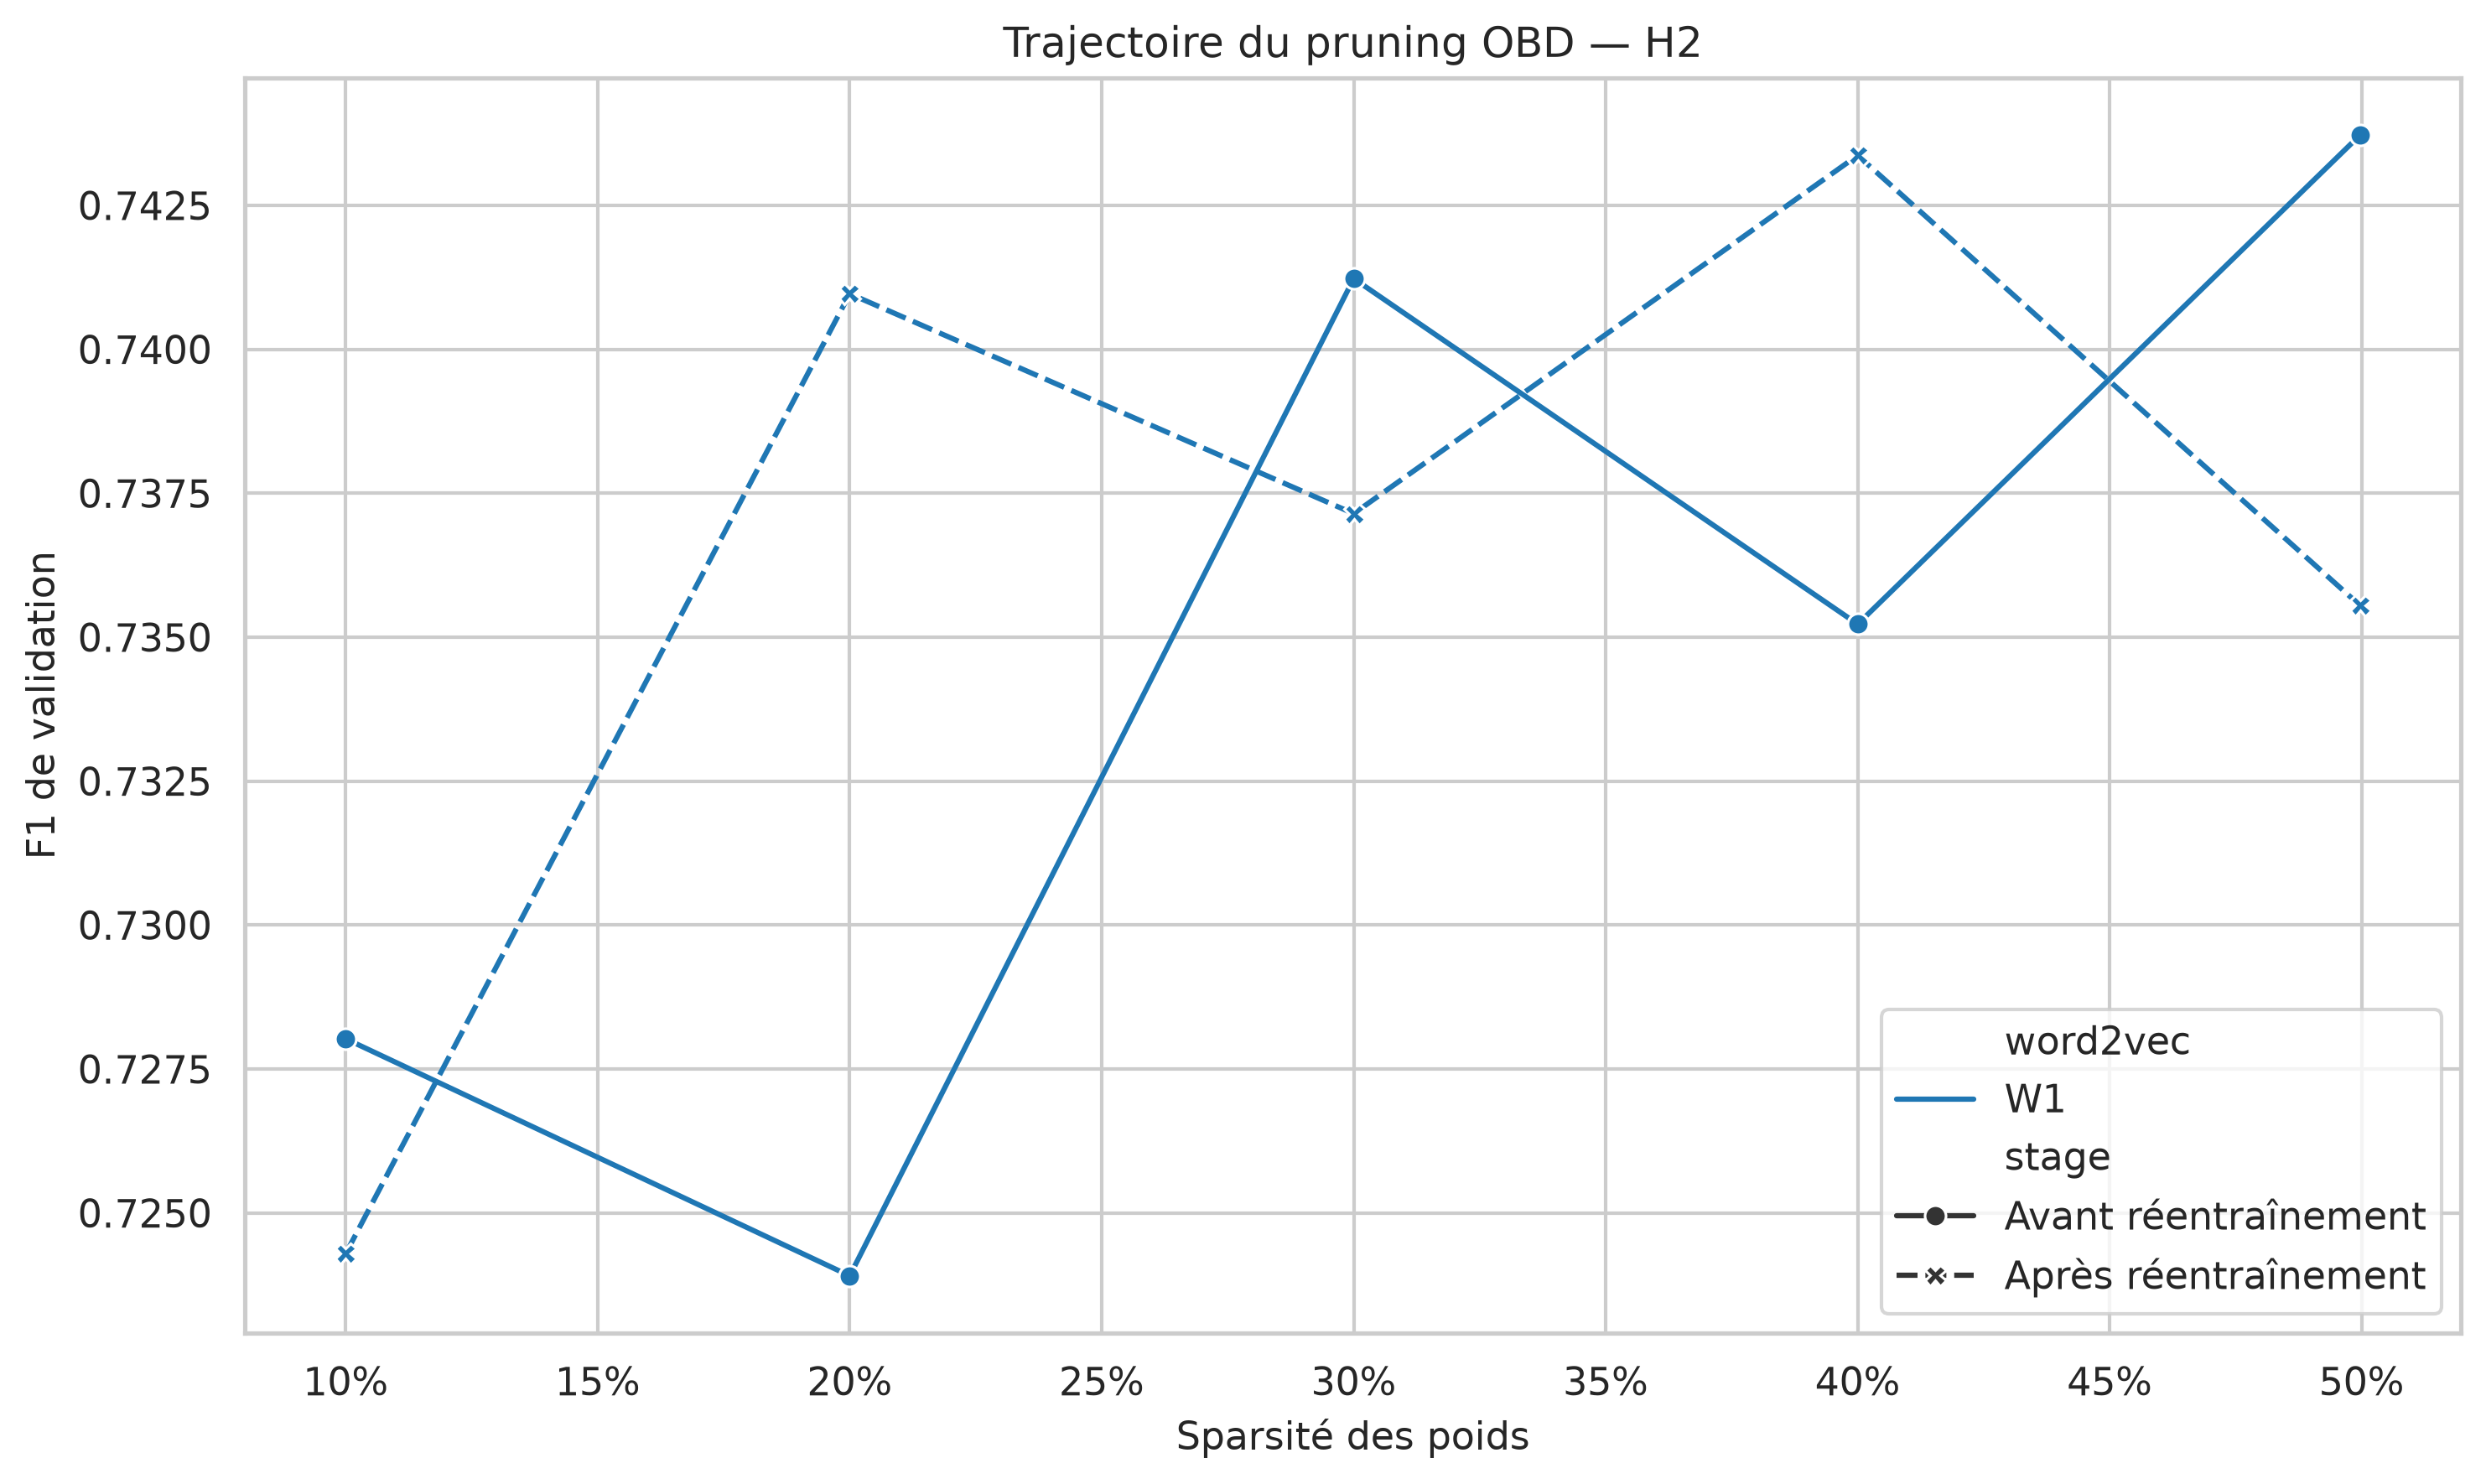
\includegraphics[width=\linewidth]{../figures/experimentales/pruning_trajectory_H2.png}
        \small (b) H2.
    \end{minipage}
    \caption{F1 de validation avant et après chaque réentraînement OBD. Les
    scores sont recalculés après chaque tour. Pour H1, un dernier micro-tour
    permet d'atteindre exactement $50\,\%$ après les arrondis en nombres entiers
    de poids.}
    \label{fig:resultats_trajectoires_obd}
\end{figure}

La trajectoire de H1 reste stable jusqu'à $40\,\%$ de sparsité. Au voisinage
de $50\,\%$, le F1 de validation passe de $0{,}6987$ juste après le cinquième
pruning à $0{,}7440$ après réentraînement : la phase de cicatrisation est ici
déterminante. H2 est moins régulier. Son F1 final vaut $0{,}7437$ avant le
dernier réentraînement et $0{,}7355$ après. Le modèle restauré minimise la
loss parmi les trois nouvelles époques, mais cette règle ne garantit ni de
surpasser l'état avant réentraînement ni de maximiser le F1. OBD préserve donc
globalement la qualité à $50\,\%$, sans rendre chaque tour individuellement
bénéfique.

\subsection{Comportement spécifique de MINT}
\label{ssec:resultats_mint}

\begin{figure}[!htbp]
    \centering
    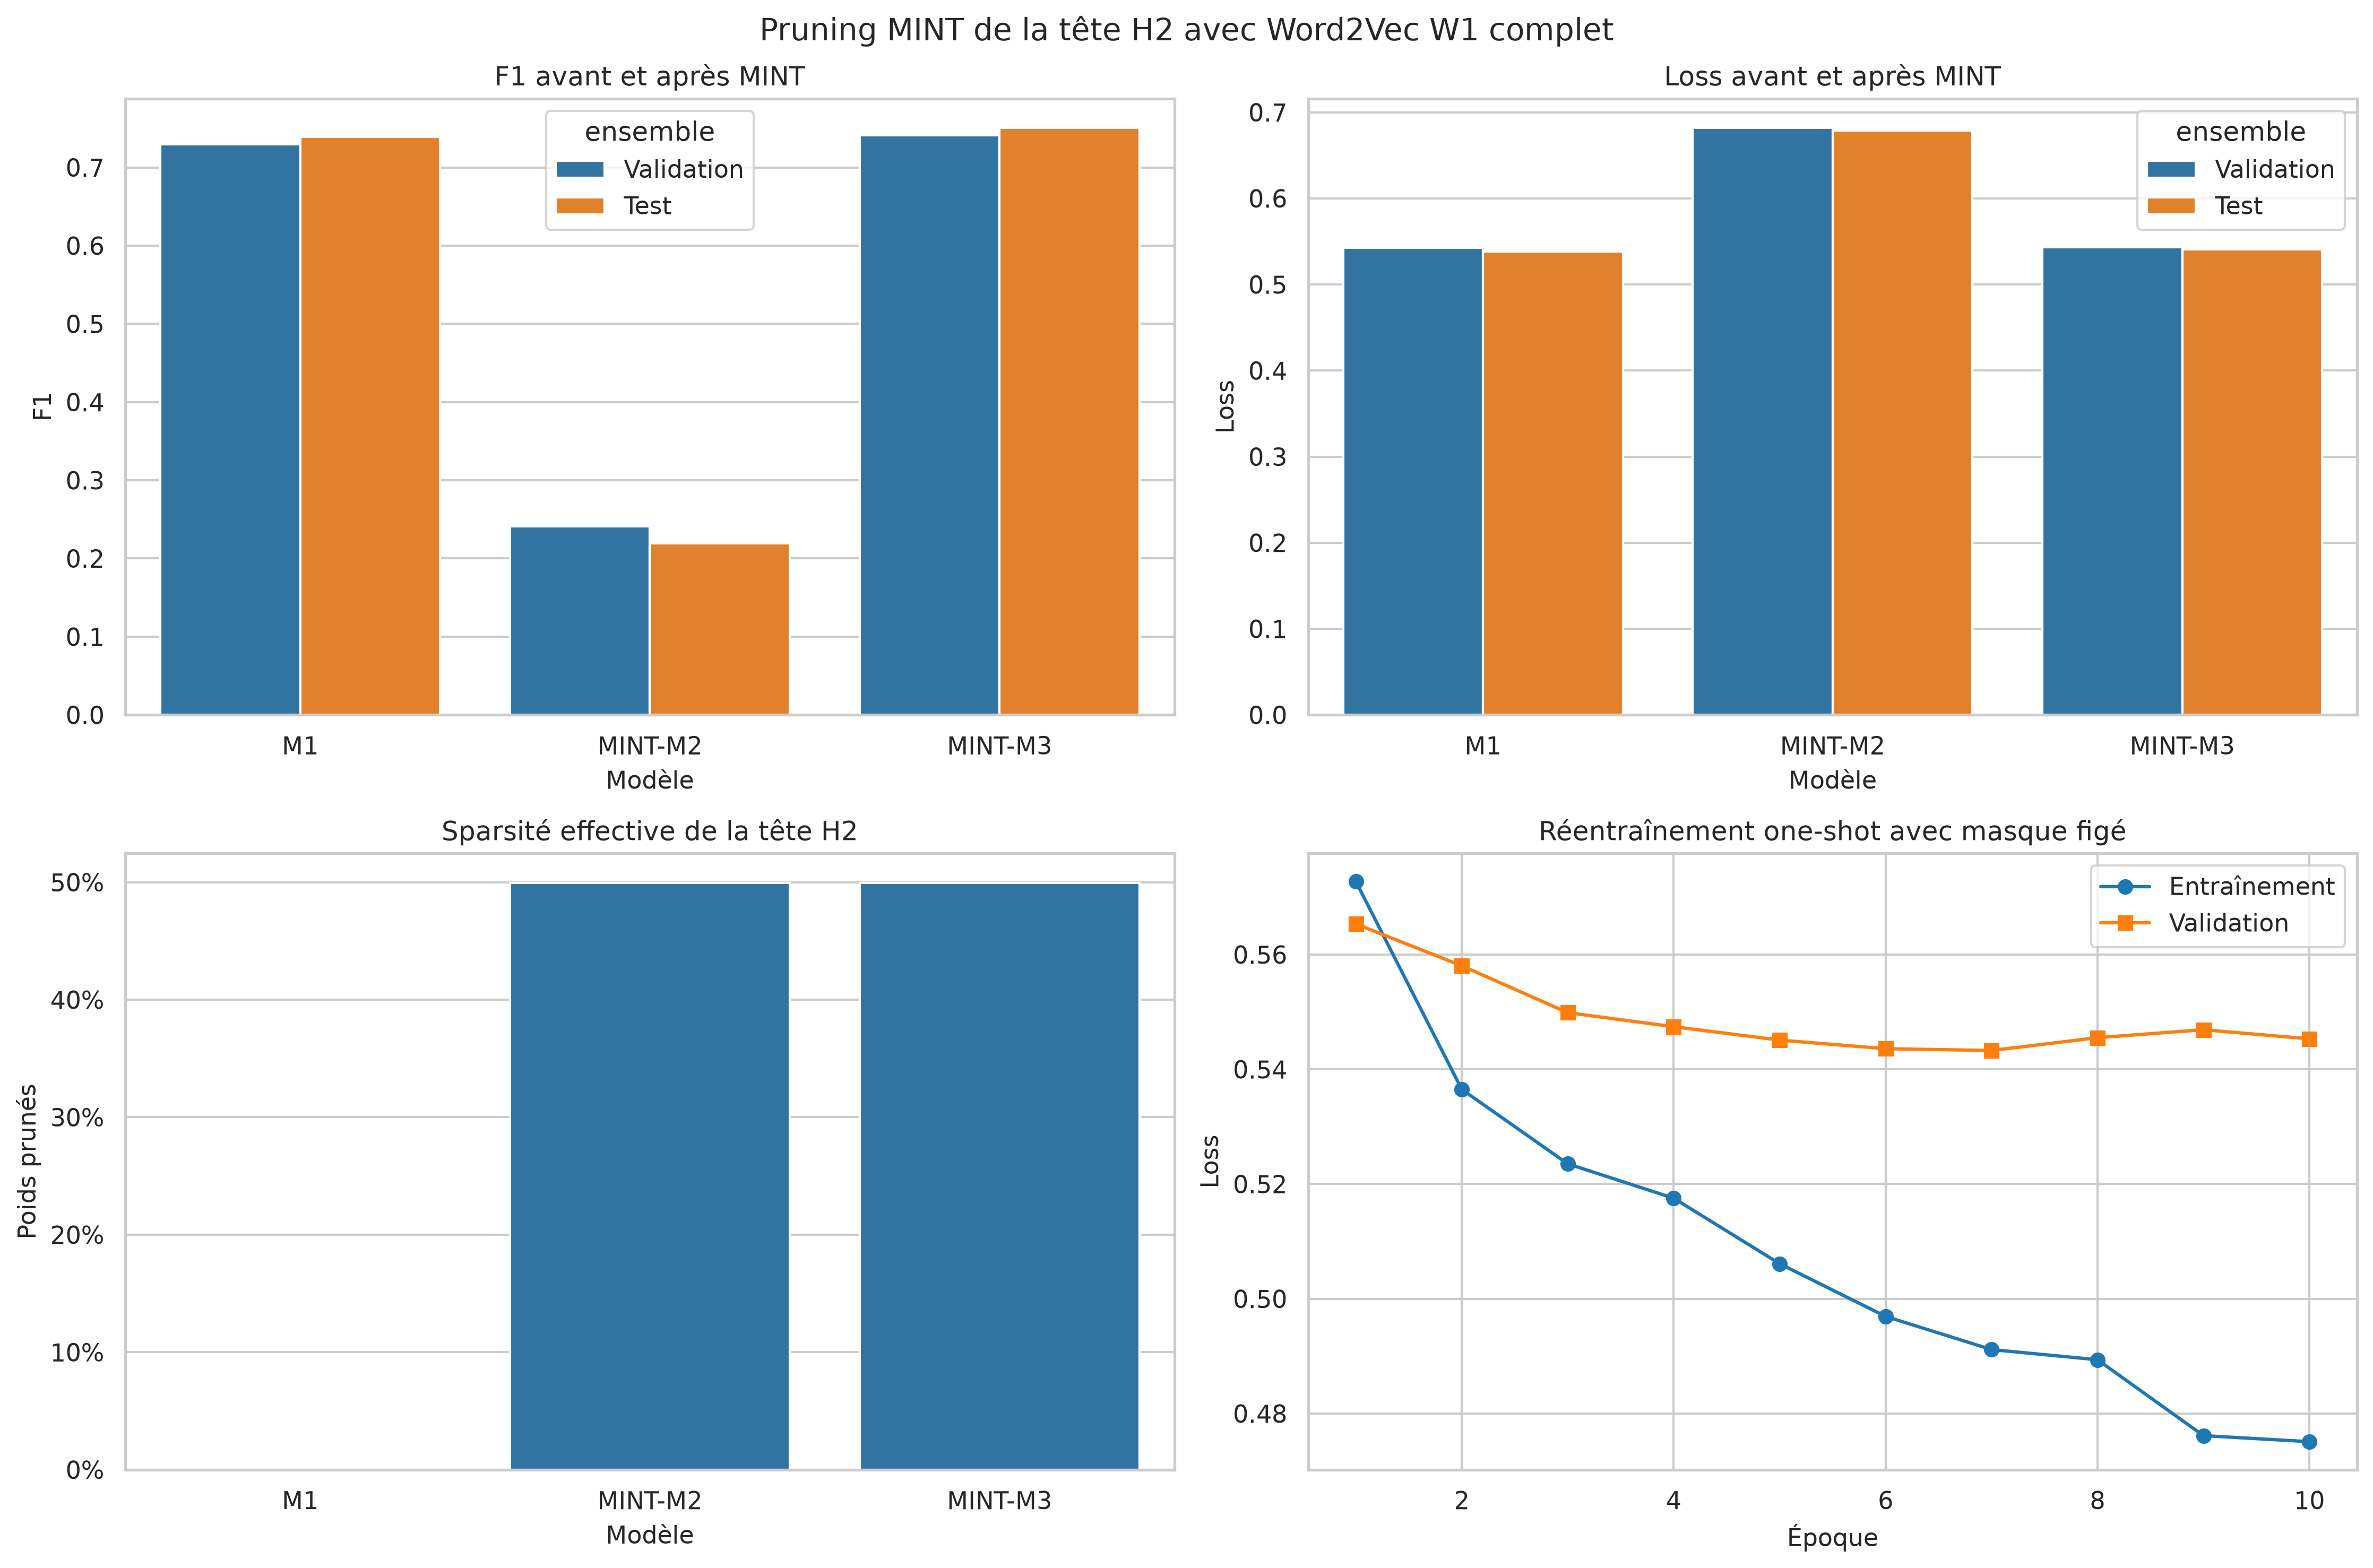
\includegraphics[width=0.94\textwidth]{../figures/experimentales/mint_summary_W1_H2.png}
    \caption{Synthèse de MINT sur H2 : F1, loss, sparsité et courbes du
    réentraînement one-shot. MINT-M2 est le modèle immédiatement masqué ;
    MINT-M3 utilise exactement le même masque après dix époques de
    réentraînement contraint.}
    \label{fig:resultats_mint_resume}
\end{figure}

La \autoref{fig:resultats_mint_resume} montre que le masque MINT modifie
fortement l'échelle des activations avant adaptation des poids restants. Le F1
et la loss de MINT-M2 se dégradent simultanément, puis MINT-M3 retrouve une loss
de test de $0{,}5409$, proche de celle de M1 ($0{,}5381$), et dépasse son F1.
La loss de validation du réentraînement atteint son minimum à l'époque 7 ;
les trois dernières époques ne l'améliorent plus. L'état restauré est donc
bien antérieur à la dernière mise à jour affichée.

\begin{figure}[!htbp]
    \centering
    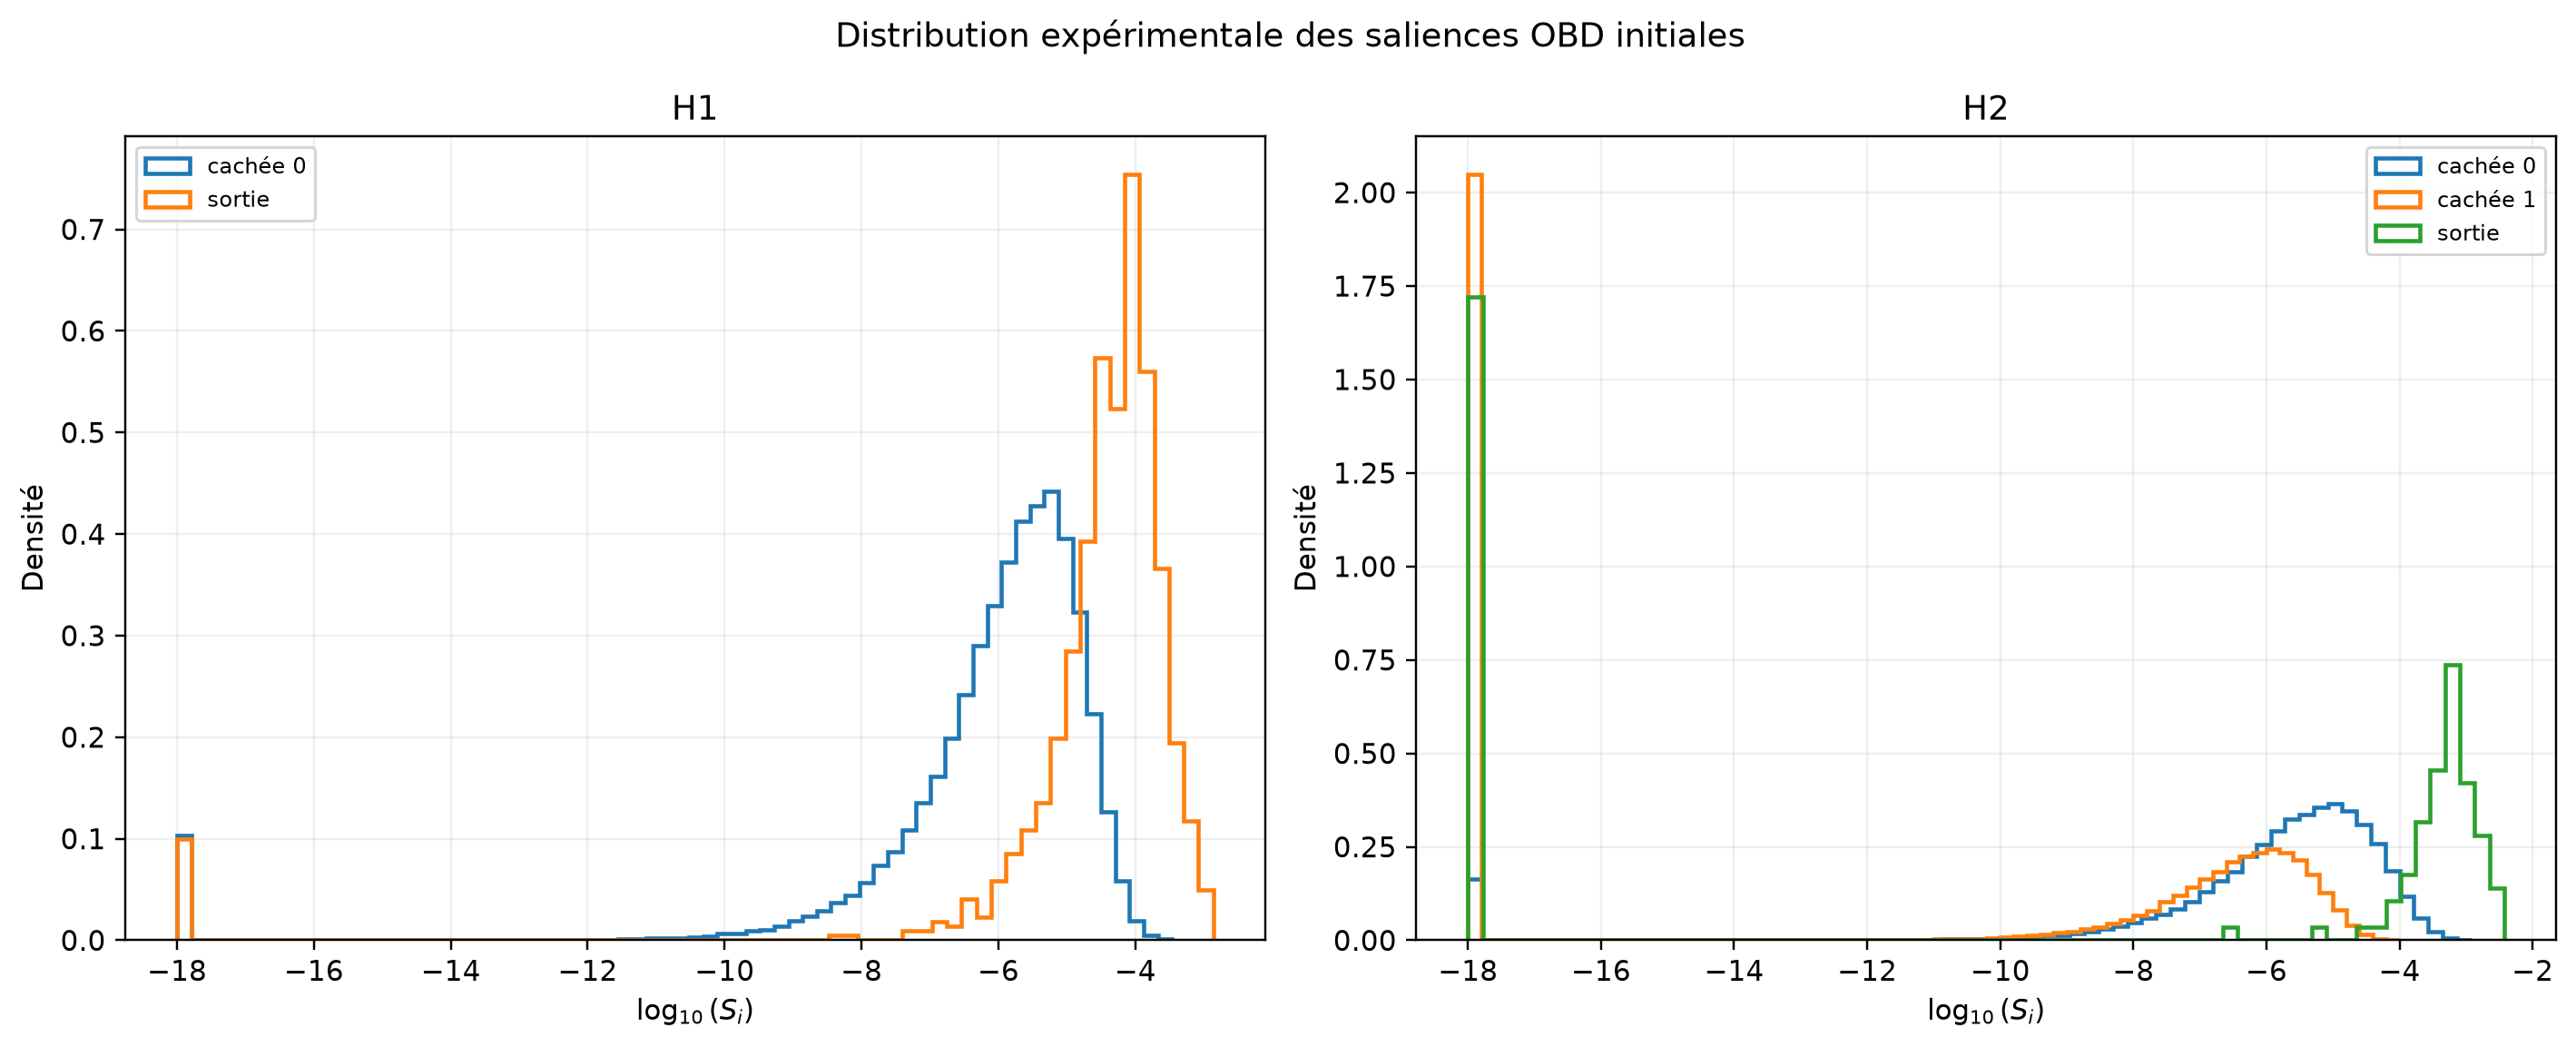
\includegraphics[width=0.94\textwidth]{../figures/experimentales/distribution_scores_obd.png}
    \par\smallskip\small (a) Saliences OBD initiales en échelle logarithmique.\par\medskip
    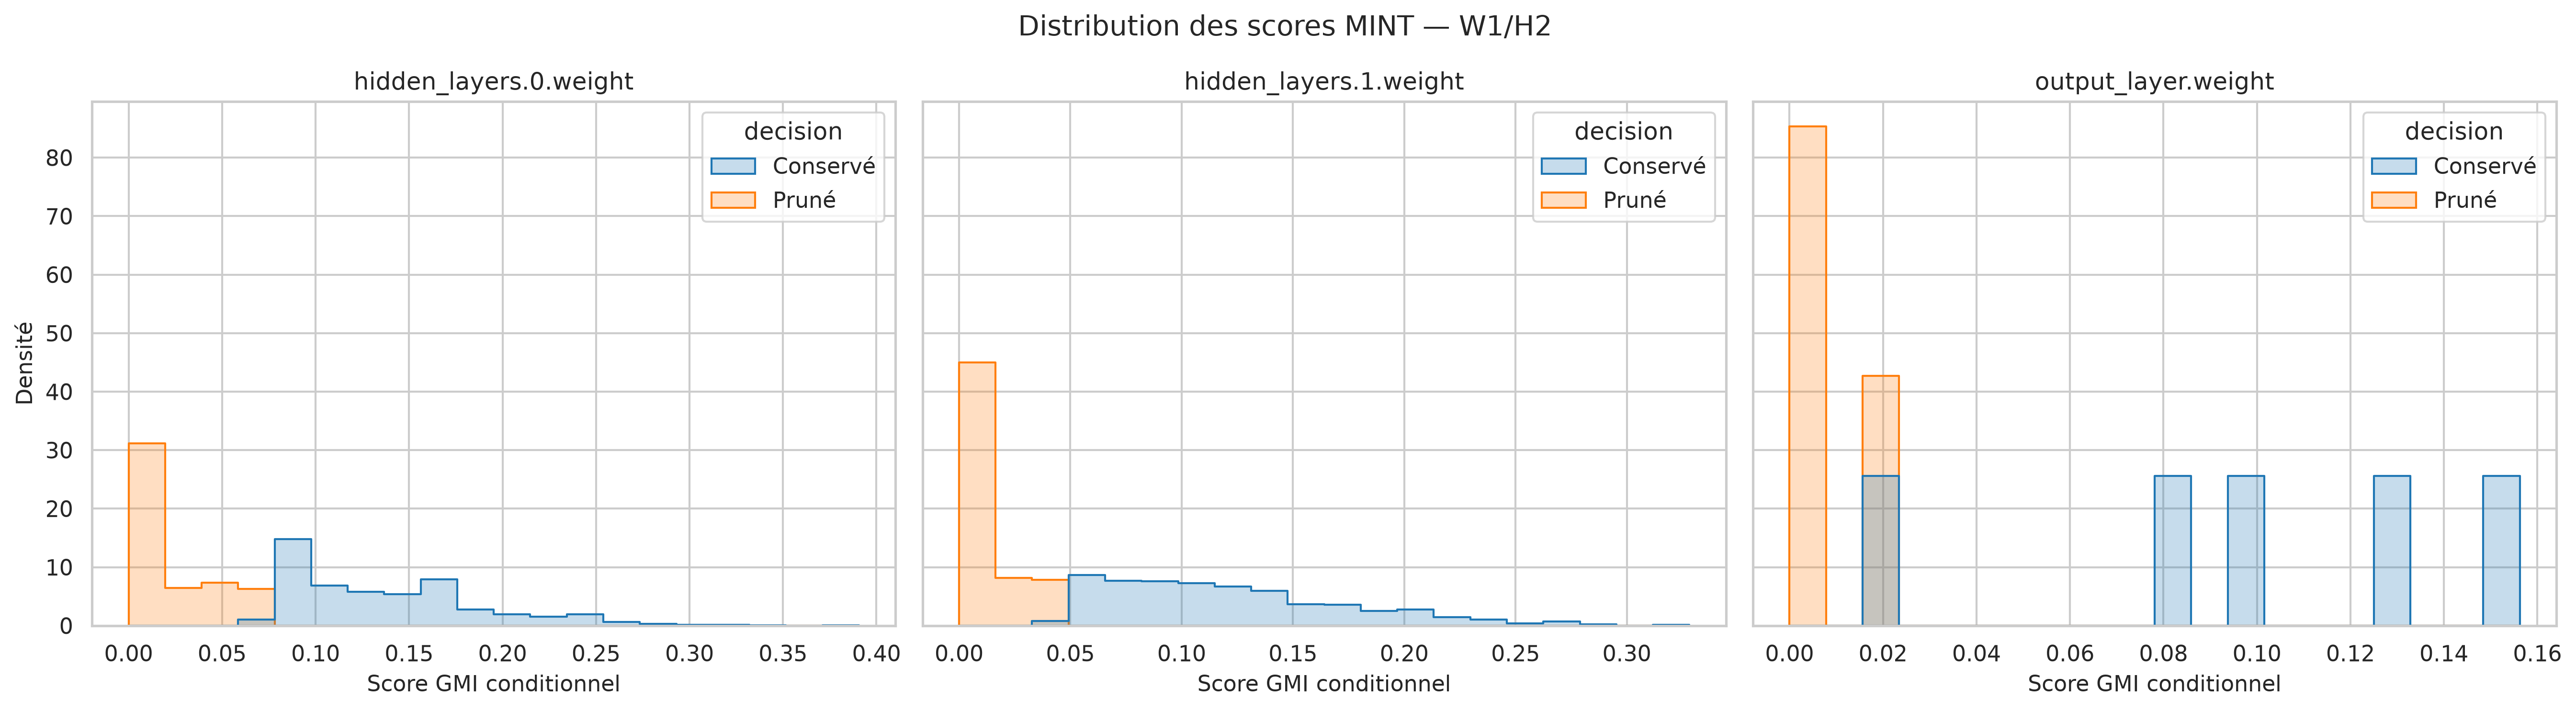
\includegraphics[width=0.98\textwidth]{../figures/experimentales/mint_score_distributions_W1_H2.png}
    \par\smallskip\small (b) Scores MINT conservés et prunés par couche.
    \caption{Distributions des scores propres aux deux méthodes. Leurs
    échelles et leurs significations diffèrent : OBD approxime une hausse
    locale de loss par poids, tandis que MINT mesure une dépendance
    conditionnelle par bloc. Une comparaison verticale directe de leurs
    valeurs brutes serait donc incorrecte.}
    \label{fig:resultats_distributions_scores}
\end{figure}

Les saliences OBD s'étendent sur de nombreux ordres de grandeur. Cette forte
asymétrie fournit une population importante de poids de très faible salience,
ce qui est cohérent avec la bonne tenue du modèle pendant les premiers tours.
Les scores MINT sont plus discrets, car l'estimateur dépend du nombre entier
d'arêtes croisées parmi $m=64$ observations. Les blocs prunés ont, par
construction, des scores plus faibles que les blocs conservés. La dernière
couche n'annule que $37{,}5\,\%$ de ses poids contre environ $50\,\%$ dans les
deux couches cachées, car elle ne contient que huit blocs et le nombre de blocs
supprimés doit être entier.

\subsection{ROC et effet du seuil de décision}
\label{ssec:resultats_roc}

\begin{figure}[!htbp]
    \centering
    \begin{minipage}[t]{0.48\textwidth}
        \centering
        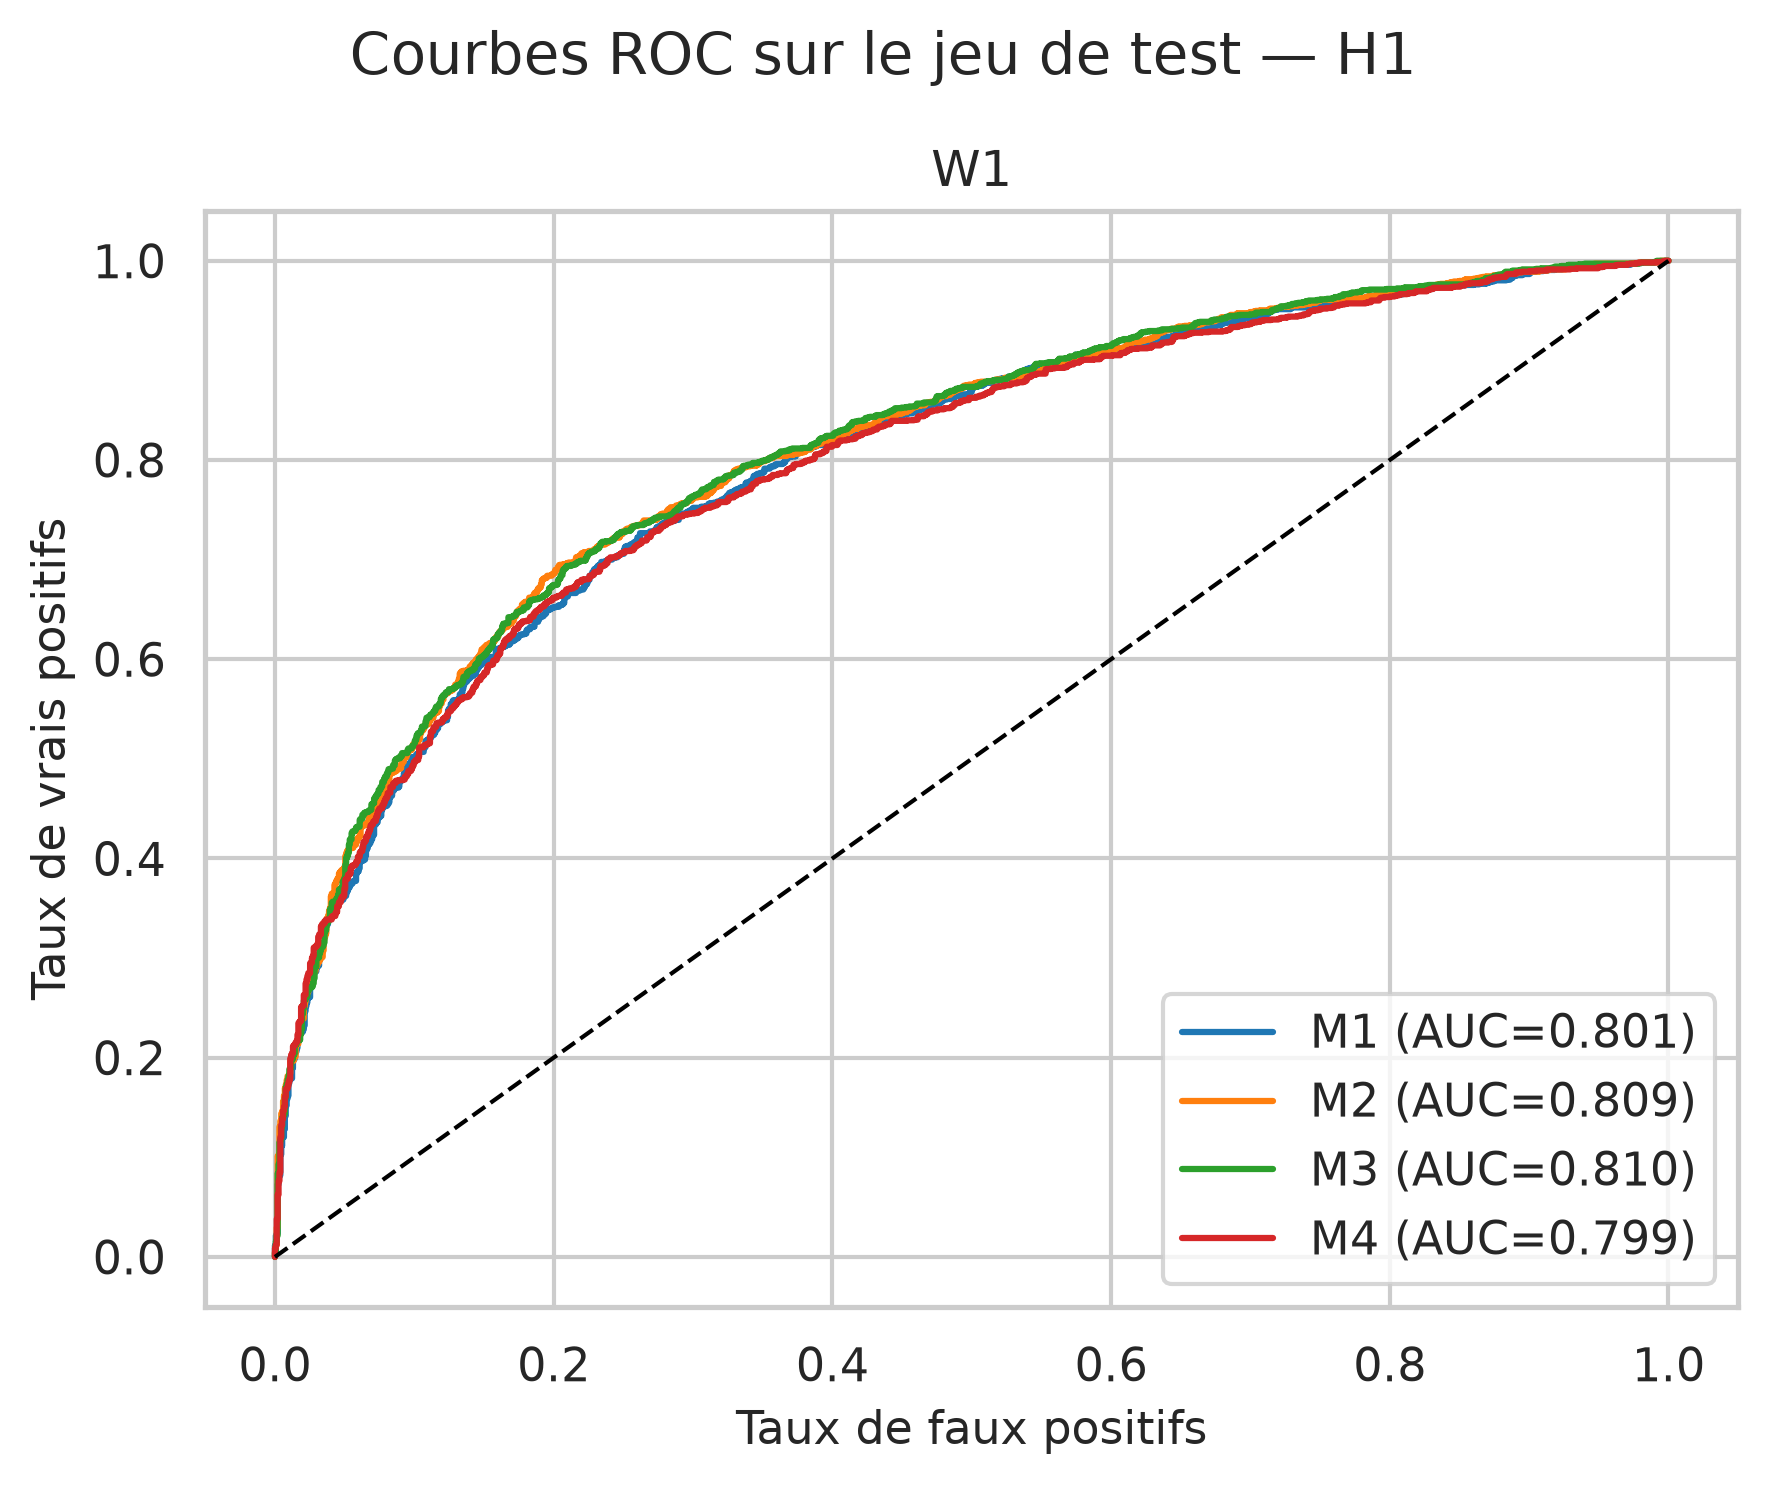
\includegraphics[width=\linewidth]{../figures/experimentales/roc_curves_H1.png}
        \small (a) H1.
    \end{minipage}
    \hfill
    \begin{minipage}[t]{0.48\textwidth}
        \centering
        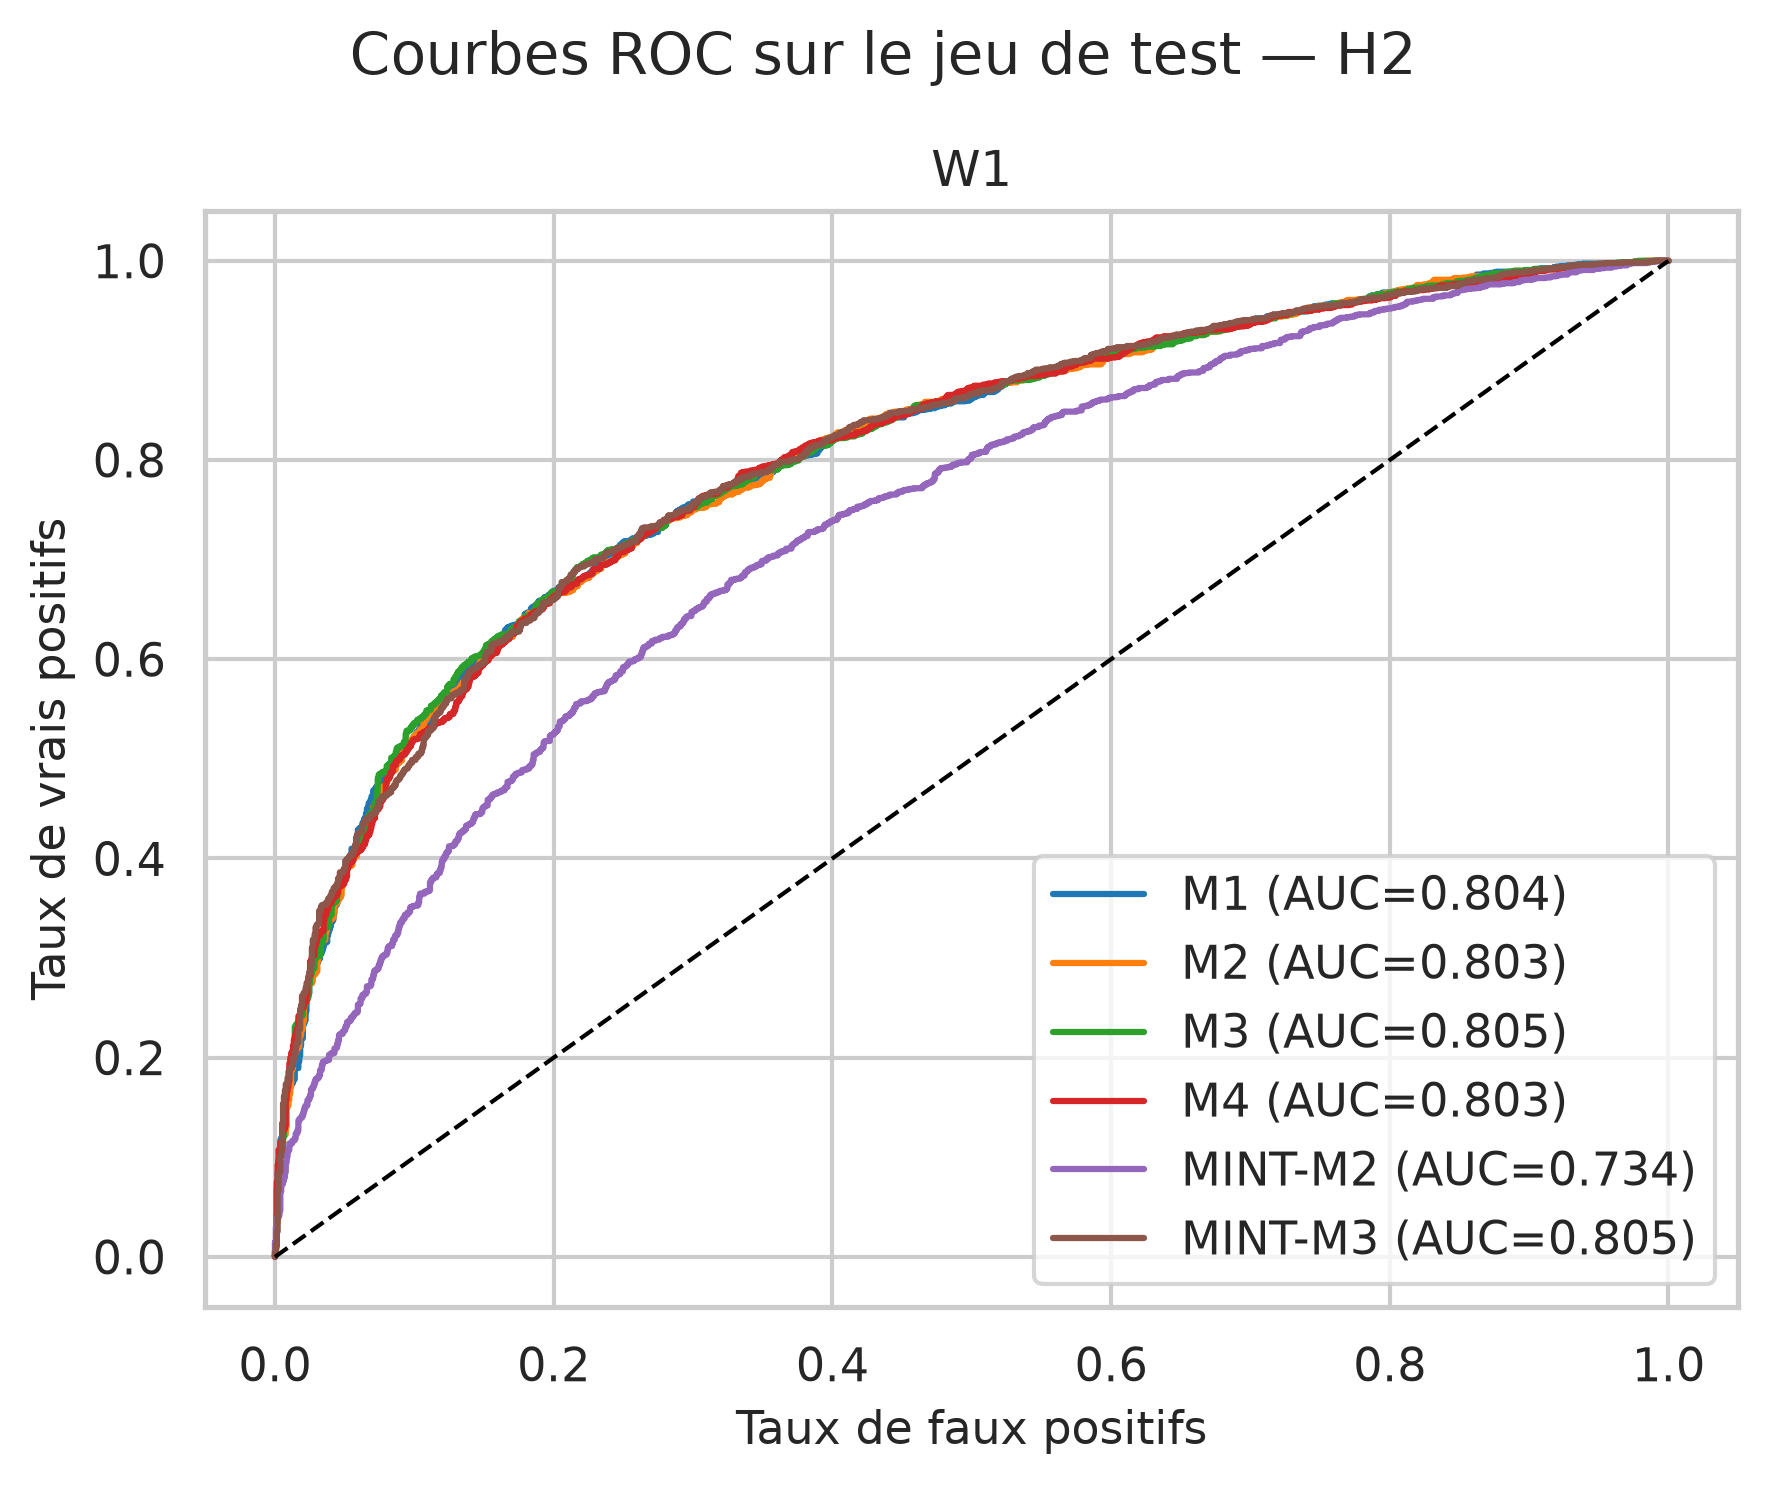
\includegraphics[width=\linewidth]{../figures/experimentales/roc_curves_H2.png}
        \small (b) H2, avec les variantes MINT.
    \end{minipage}
    \caption{Courbes ROC sur le jeu de test. L'aire sous la courbe mesure le
    classement des exemples sur tous les seuils, contrairement au F1 et à
    l'accuracy calculés au seuil fixe $0{,}5$.}
    \label{fig:resultats_roc}
\end{figure}

Les variantes finales de H1 ont des ROC-AUC comprises entre $0{,}7989$ et
$0{,}8102$, et celles de H2 entre $0{,}8027$ et $0{,}8048$. Les courbes sont
donc proches malgré les différences de F1. MINT-M2 constitue l'exception : son
ROC-AUC de $0{,}7336$ reste supérieure au hasard alors que son F1 vaut seulement
$0{,}2192$. Une partie de son effondrement provient ainsi du seuil et de la
calibration, mais la baisse d'AUC montre qu'il perd aussi une capacité de
classement. MINT-M3 restaure les deux aspects.

\subsection{Compromis qualité--mémoire et qualité--calcul}
\label{ssec:resultats_pareto}

\begin{figure}[!htbp]
    \centering
    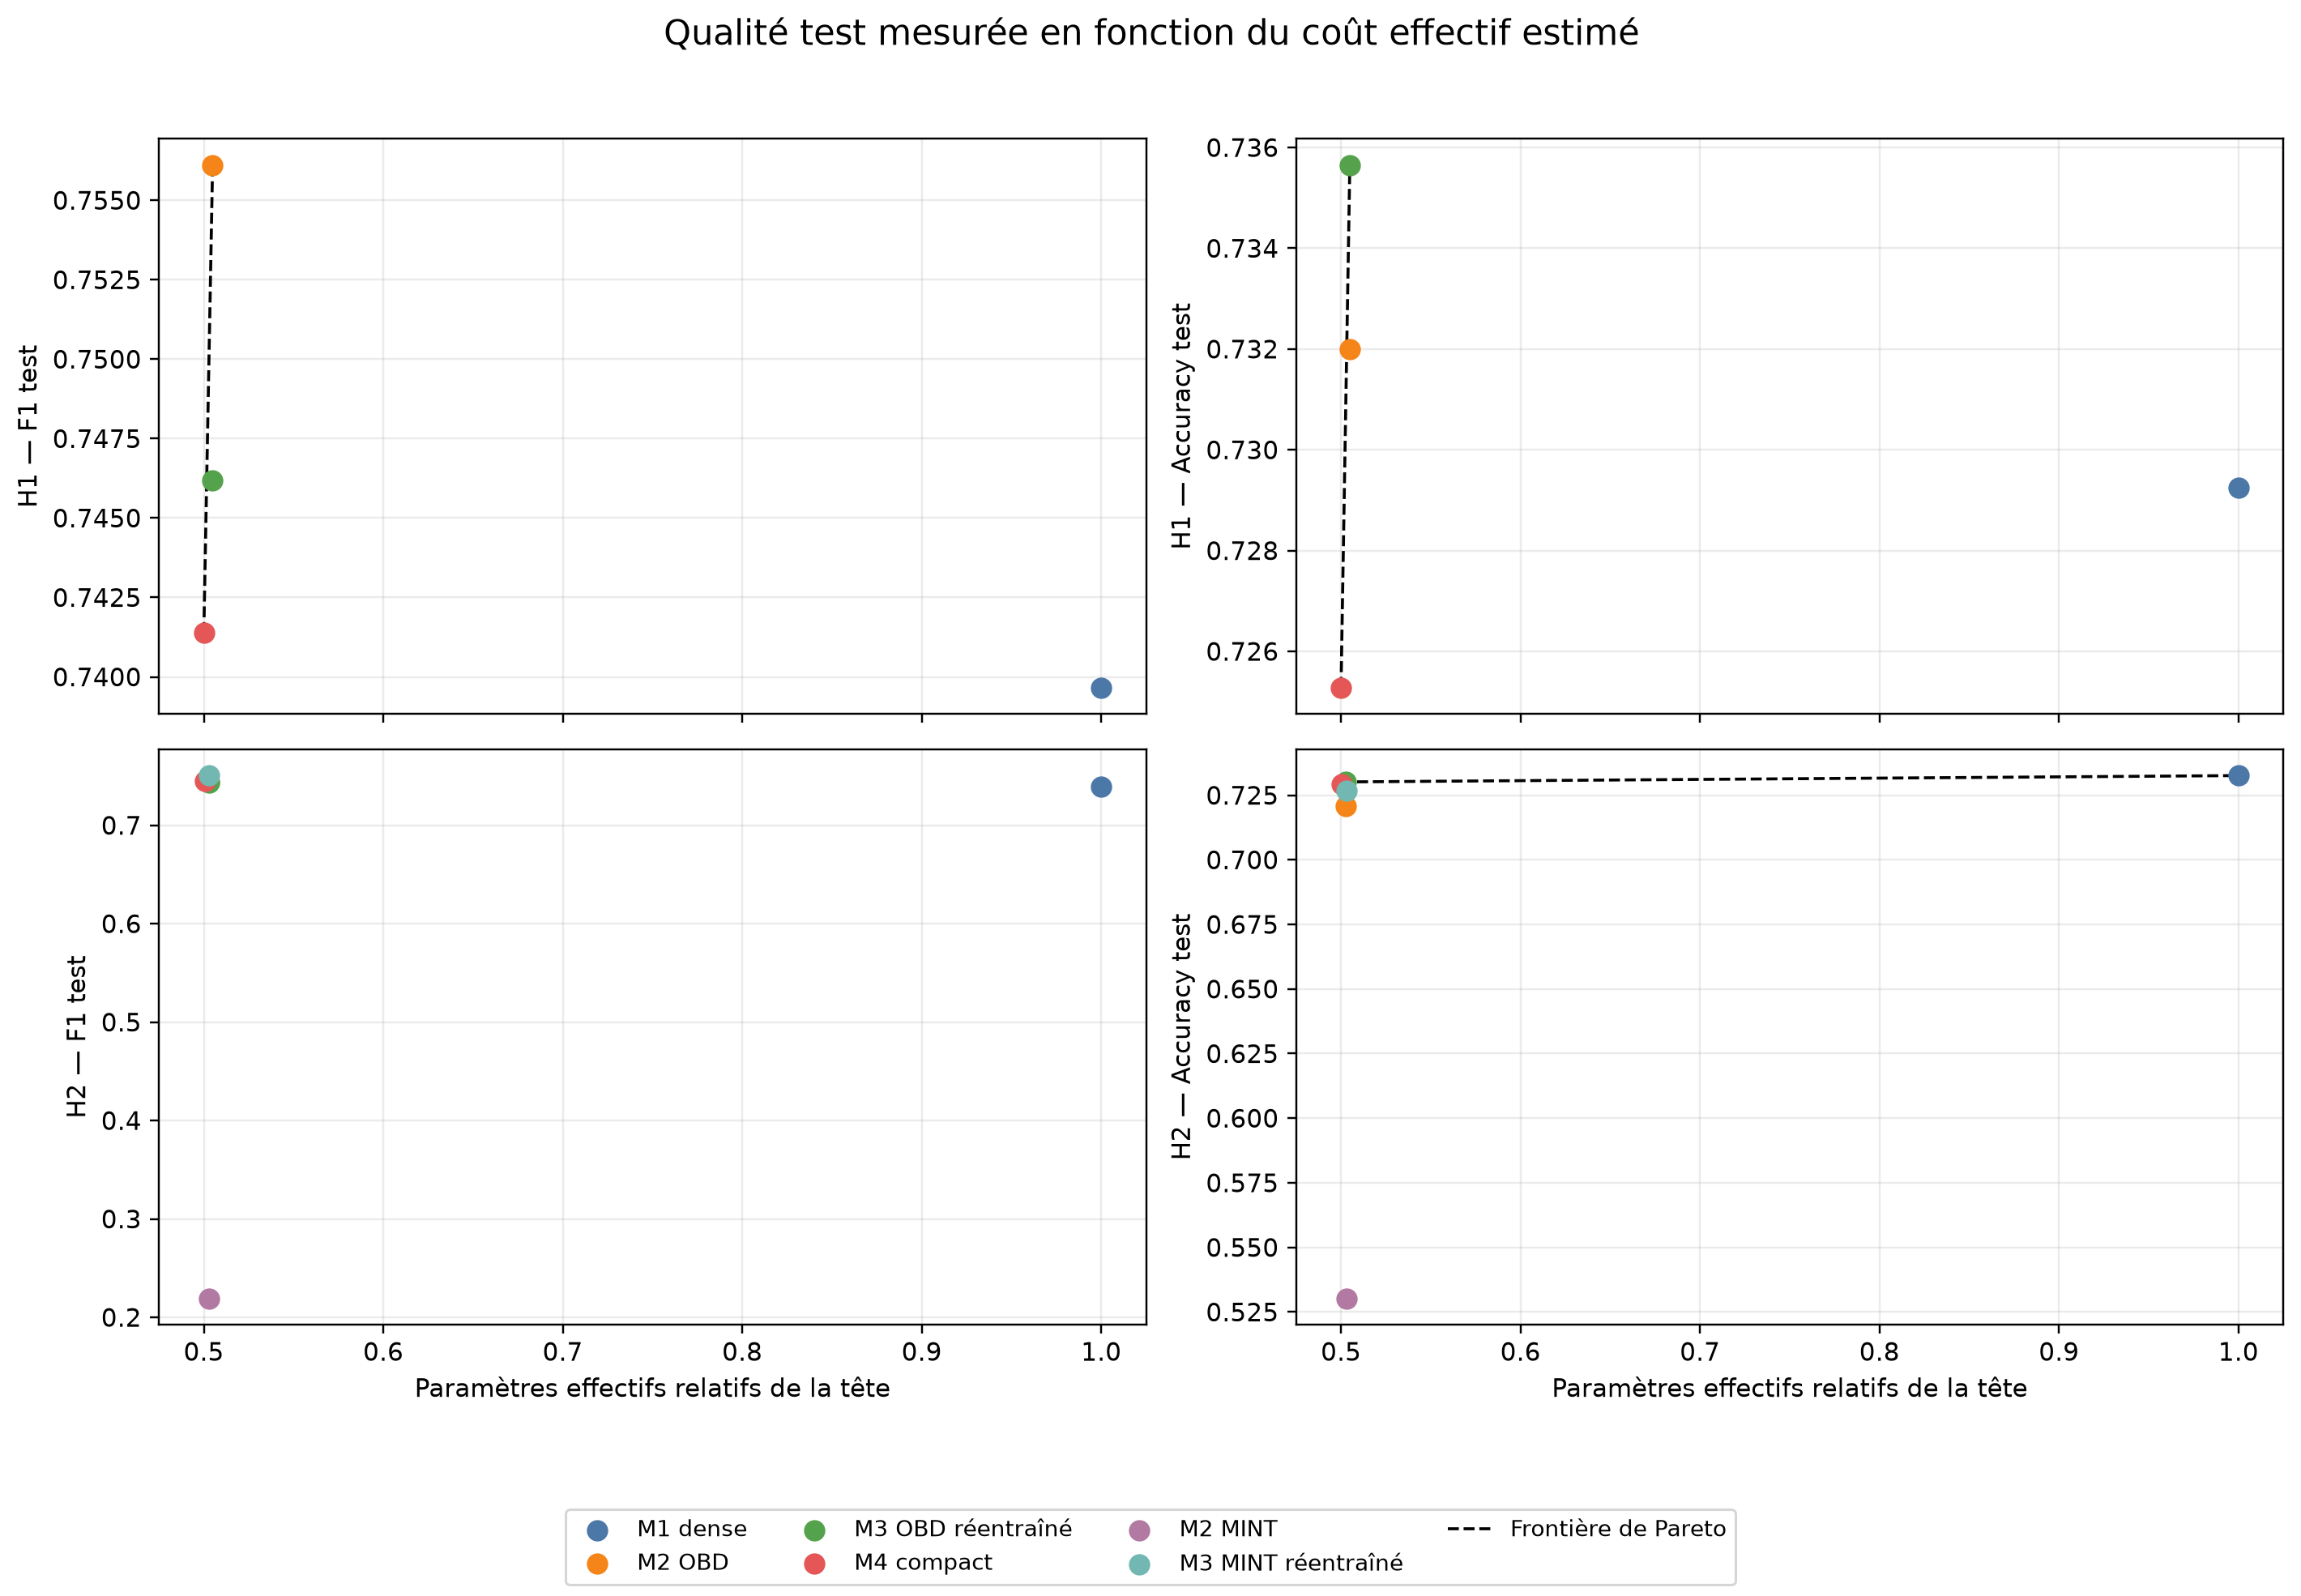
\includegraphics[width=0.96\textwidth]{../figures/experimentales/qualite_memoire_tete_pareto.png}
    \caption{F1 et accuracy de test en fonction des paramètres effectifs de
    la tête, normalisés par M1. Les pointillés relient les solutions non
    dominées. M4 est compté avec ses dimensions physiques réduites ; M2 et M3
    sont comptés selon leur nombre idéal de poids actifs.}
    \label{fig:resultats_pareto_memoire_tete}
\end{figure}

\begin{figure}[!htbp]
    \centering
    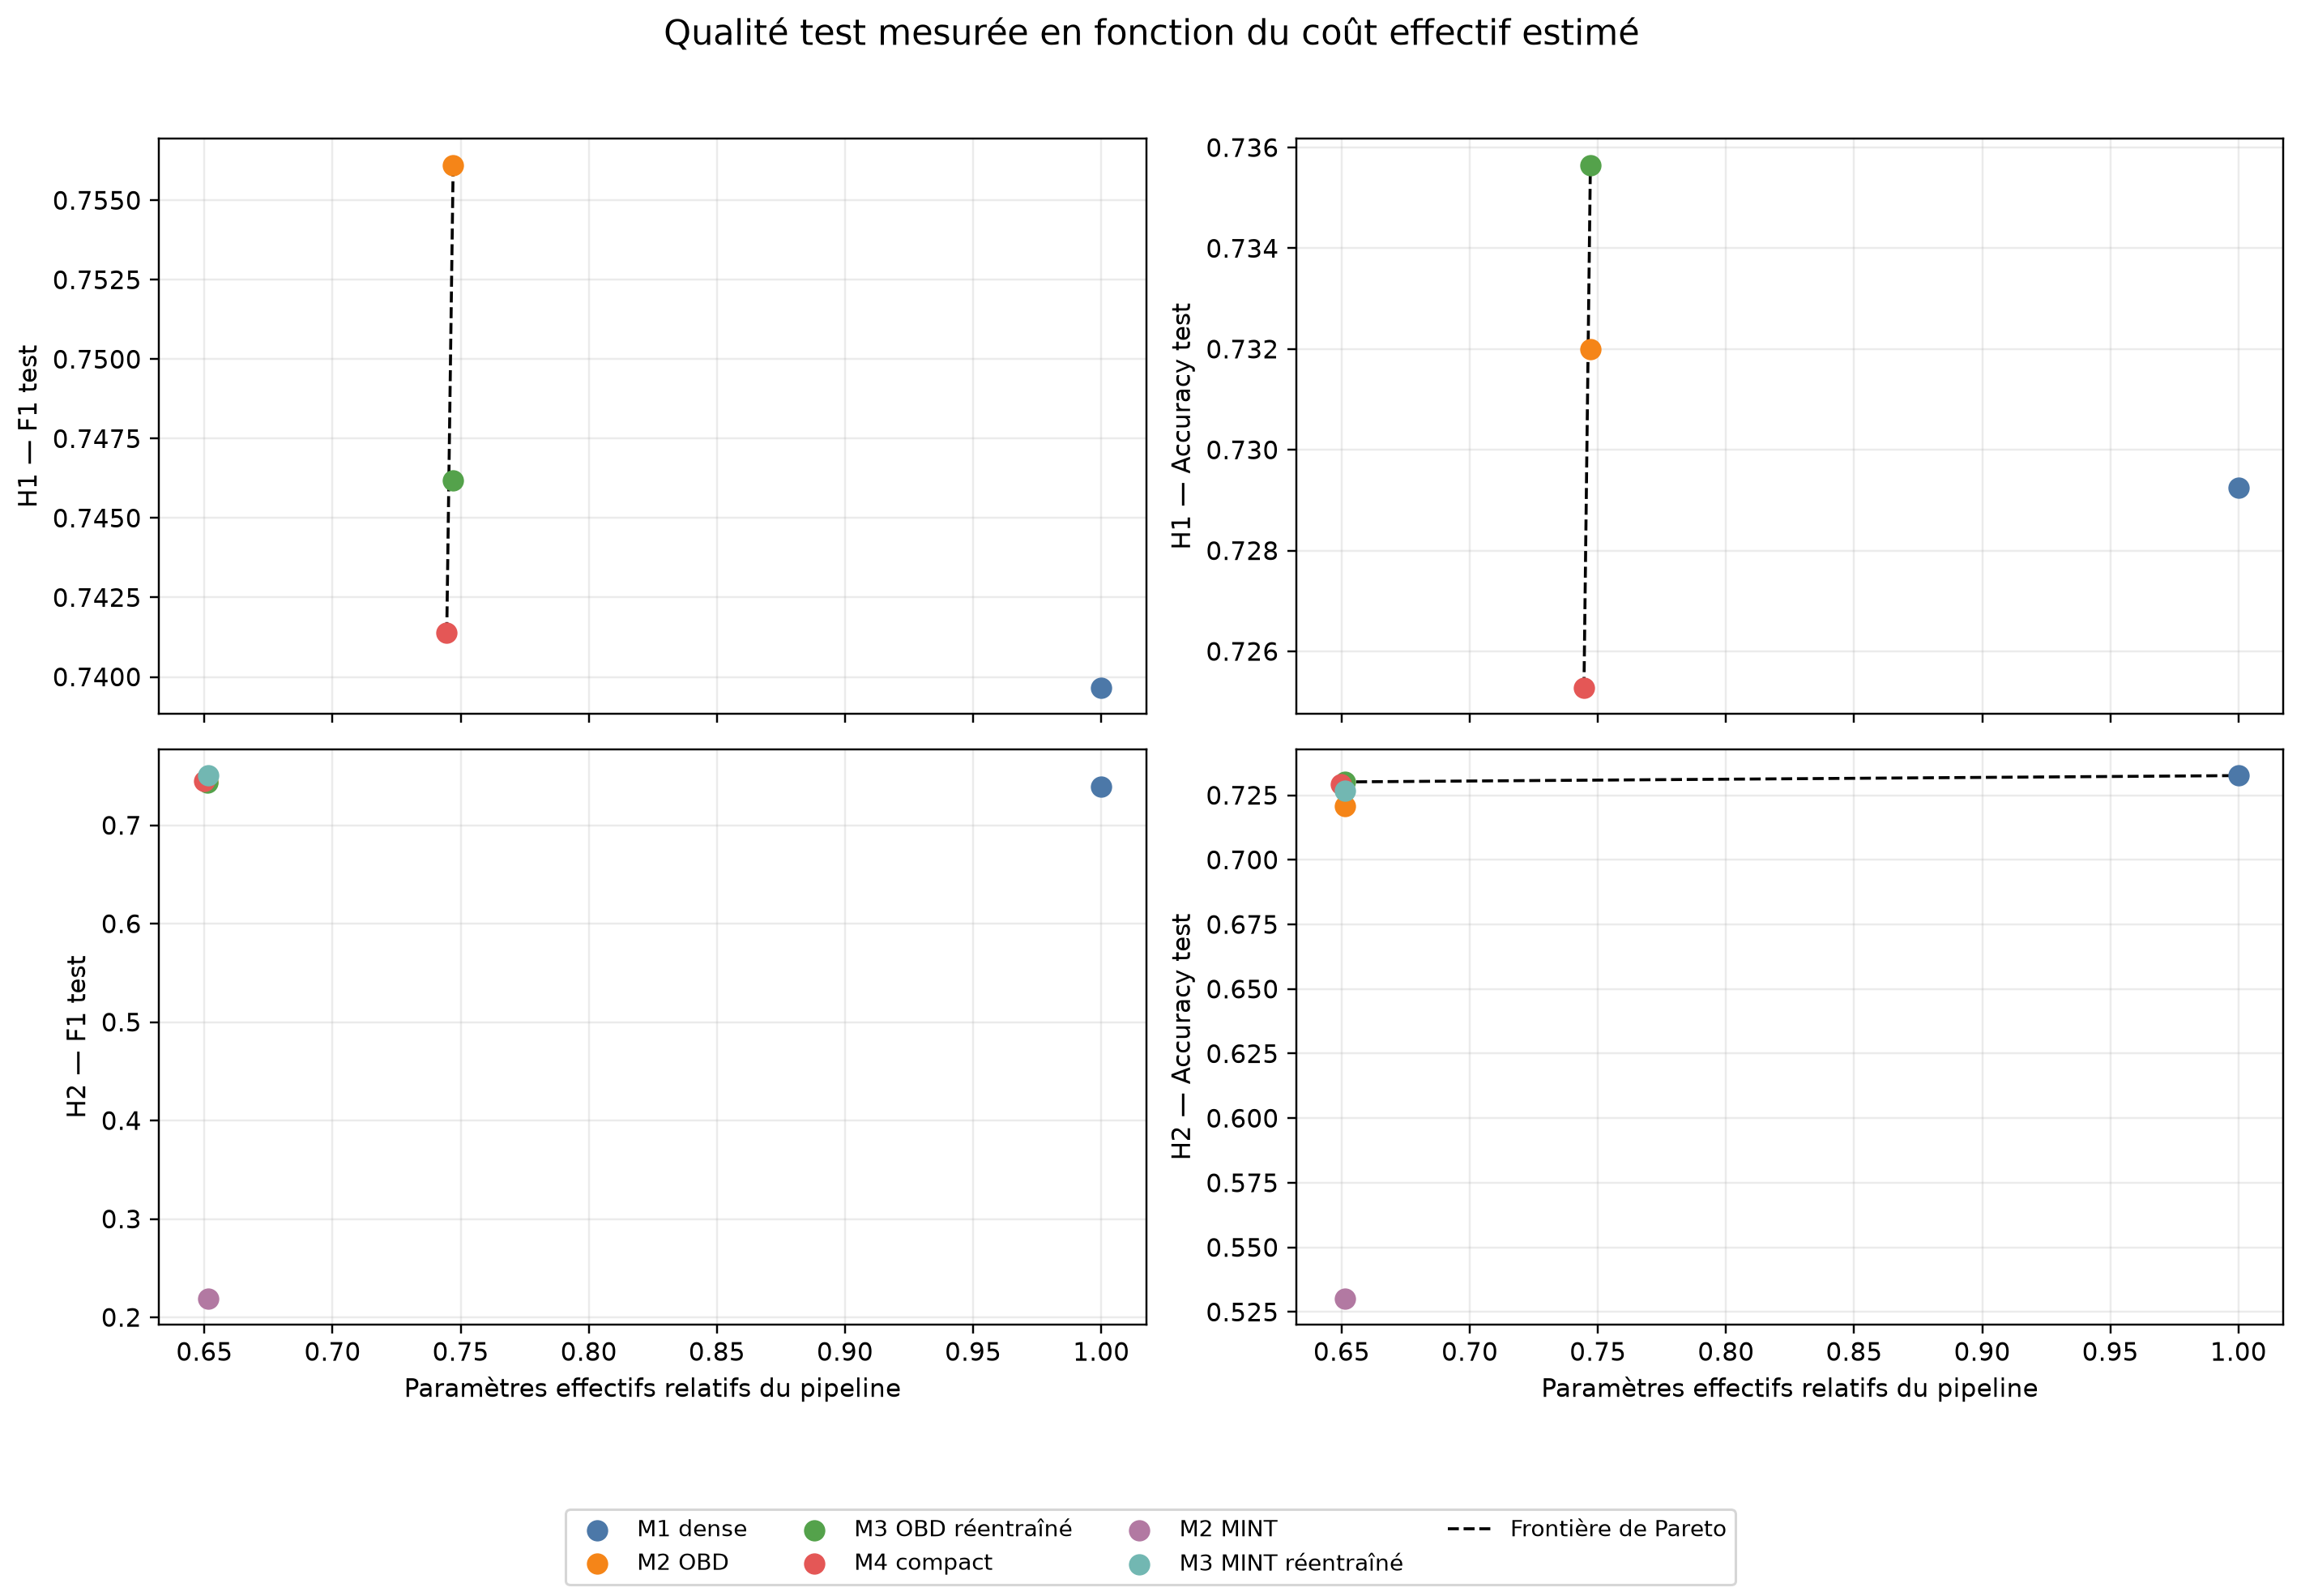
\includegraphics[width=0.96\textwidth]{../figures/experimentales/qualite_memoire_pipeline_pareto.png}
    \caption{Même compromis en incluant les $100\,000$ paramètres fixes de
    W1. Les modèles H1 compressés conservent environ $74{,}5\,\%$ du coût de
    M1 ; les modèles H2 compressés en conservent environ $65\,\%$. MINT-M2 est
    dominé en raison de sa forte perte de qualité.}
    \label{fig:resultats_pareto_memoire_pipeline}
\end{figure}

\begin{figure}[!htbp]
    \centering
    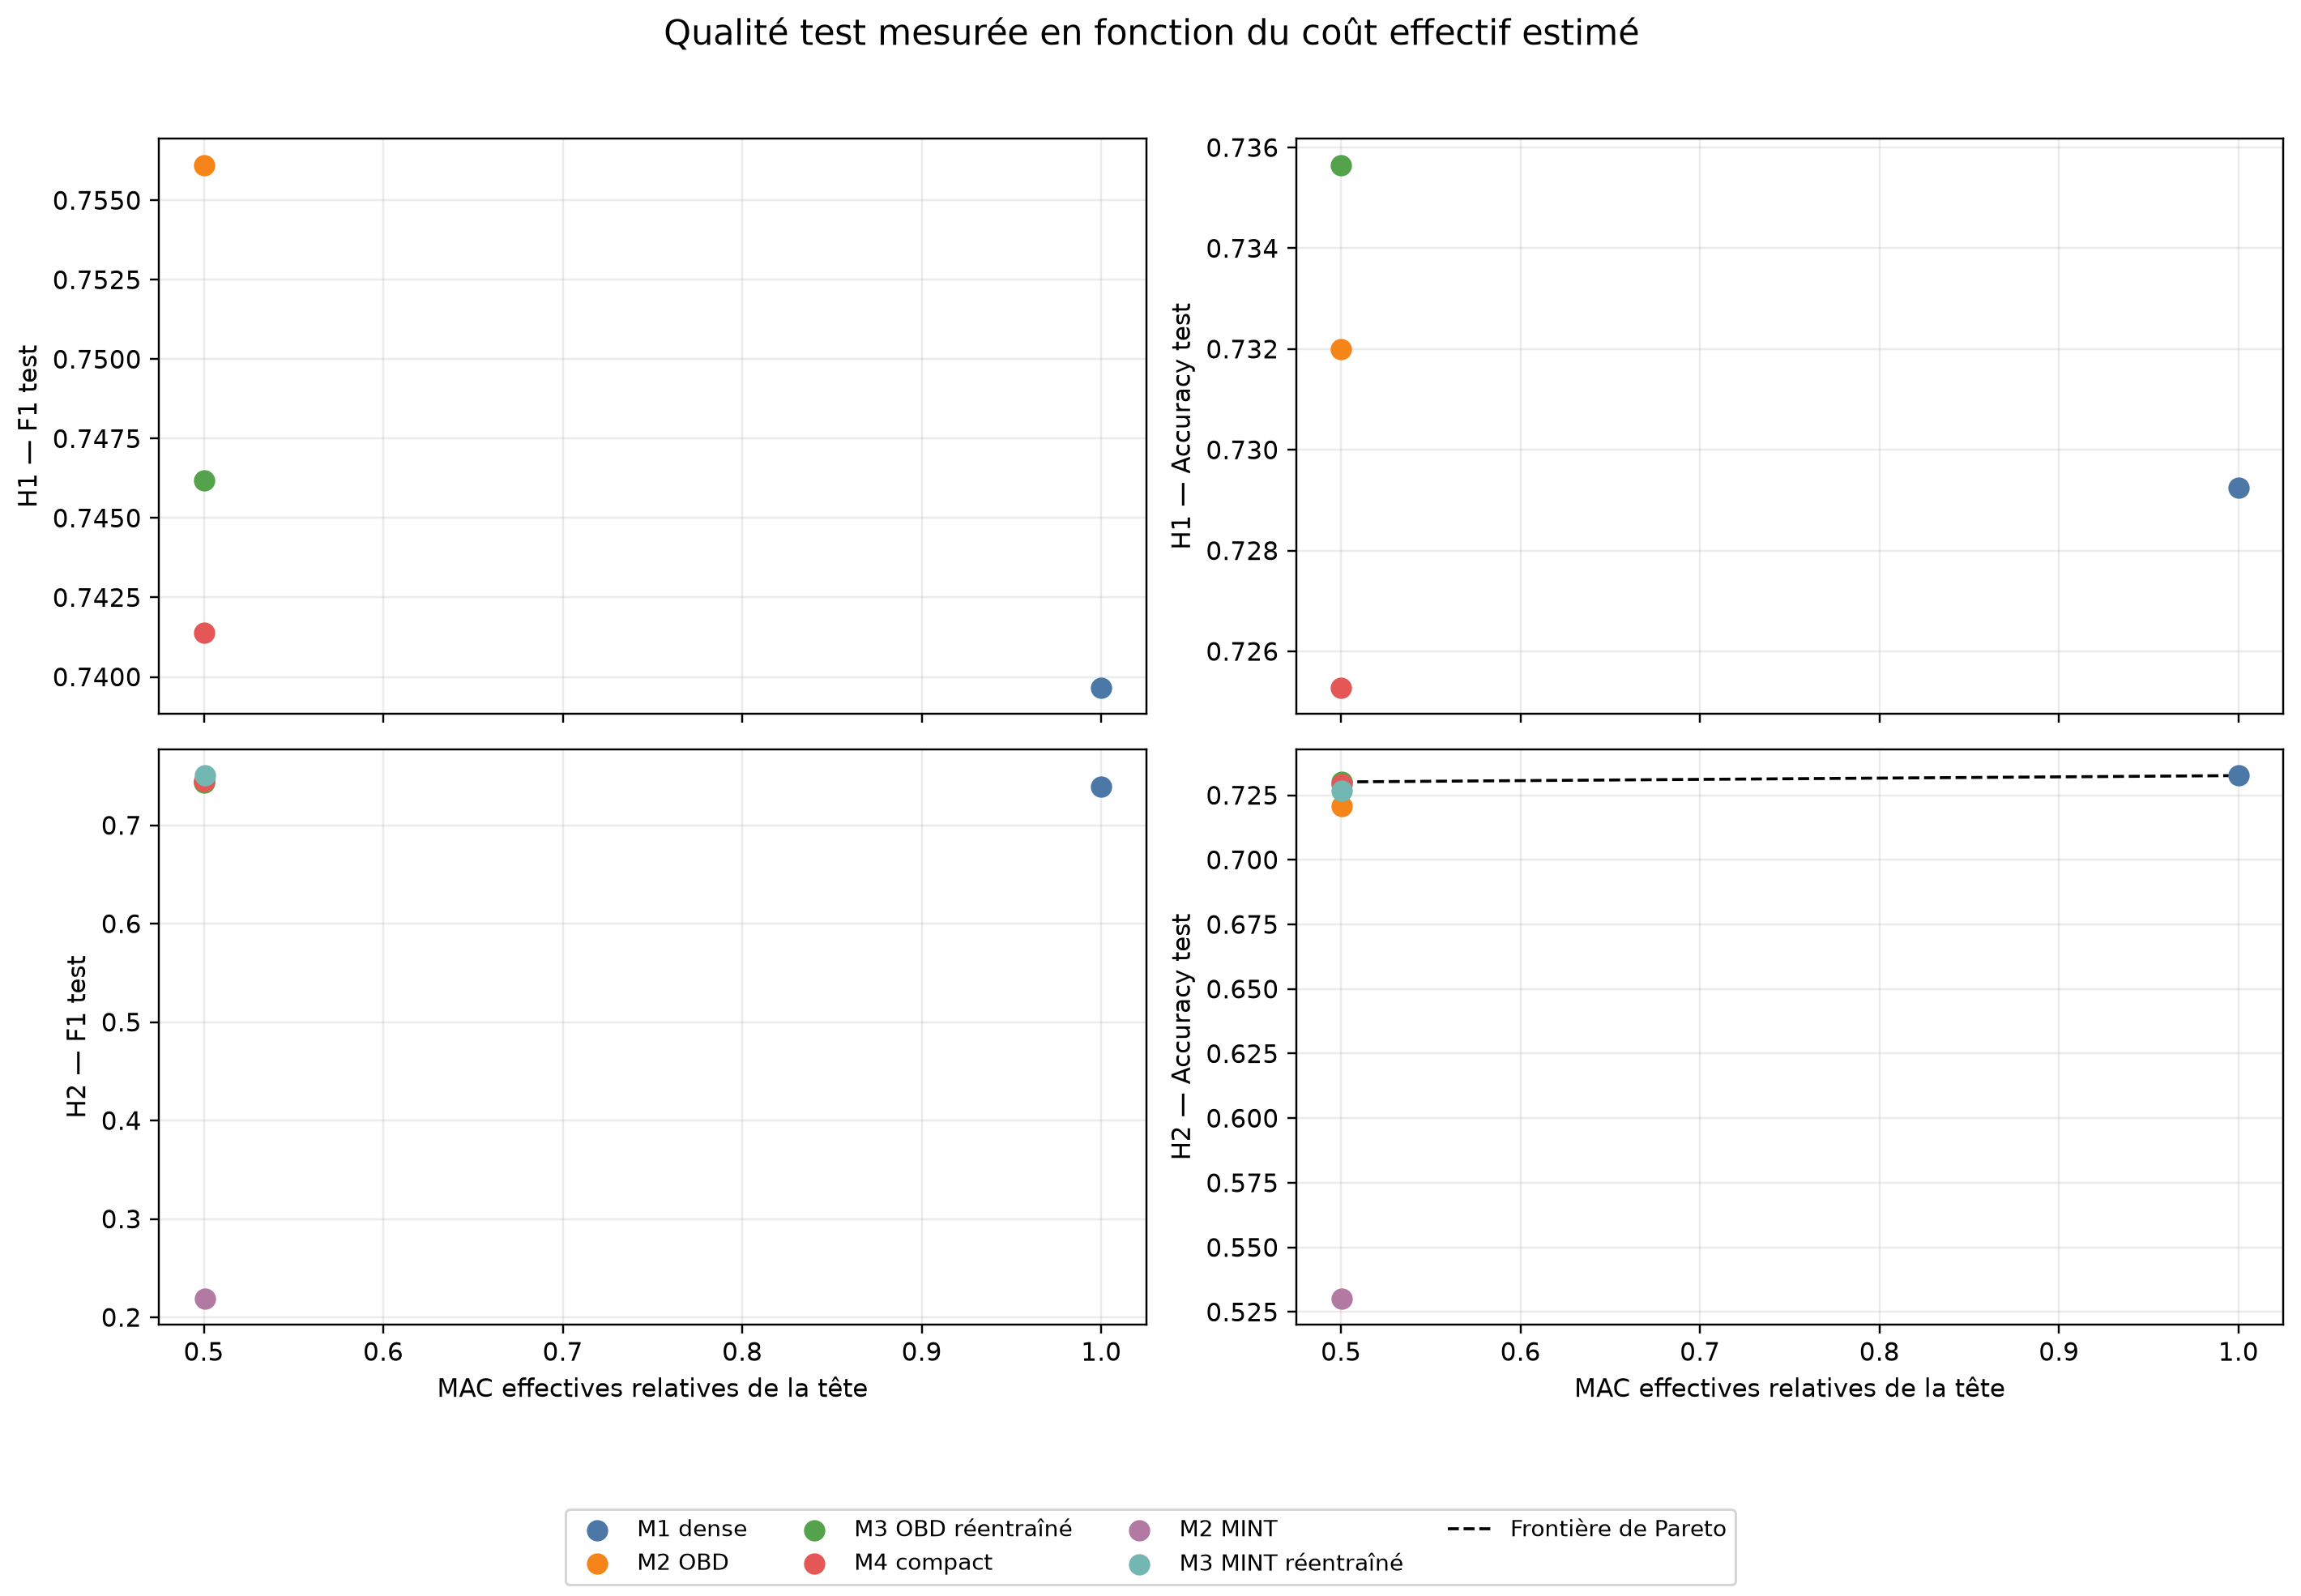
\includegraphics[width=0.96\textwidth]{../figures/experimentales/qualite_calcul_tete_pareto.png}
    \caption{Qualité de test en fonction des MAC effectives idéales de la
    tête. Pour les masques OBD et MINT, l'abscisse suppose qu'un moteur sparse
    sait omettre les multiplications par zéro ; elle ne représente donc pas la
    quantité de calcul réellement exécutée par PyTorch dense.}
    \label{fig:resultats_pareto_calcul}
\end{figure}

Dans la vue tête seule, toutes les solutions réduites se situent près de
$50\,\%$ du coût de M1. La qualité permet alors de les départager : H1/M2 et
H2/MINT-M3 maximisent le F1, tandis que H1/M3 et H2/M1 maximisent l'accuracy.
Le passage à la vue pipeline rapproche horizontalement les solutions de M1,
mais ne change pas leur ordre. Ces courbes répondent à la question du nombre
de paramètres ou de MAC \emph{potentiellement} évitables ; elles ne suffisent
pas à conclure sur le déploiement.

\subsection{Critères ajustés et sensibilité au coefficient alpha}
\label{ssec:resultats_ajustes}

\begin{figure}[!htbp]
    \centering
    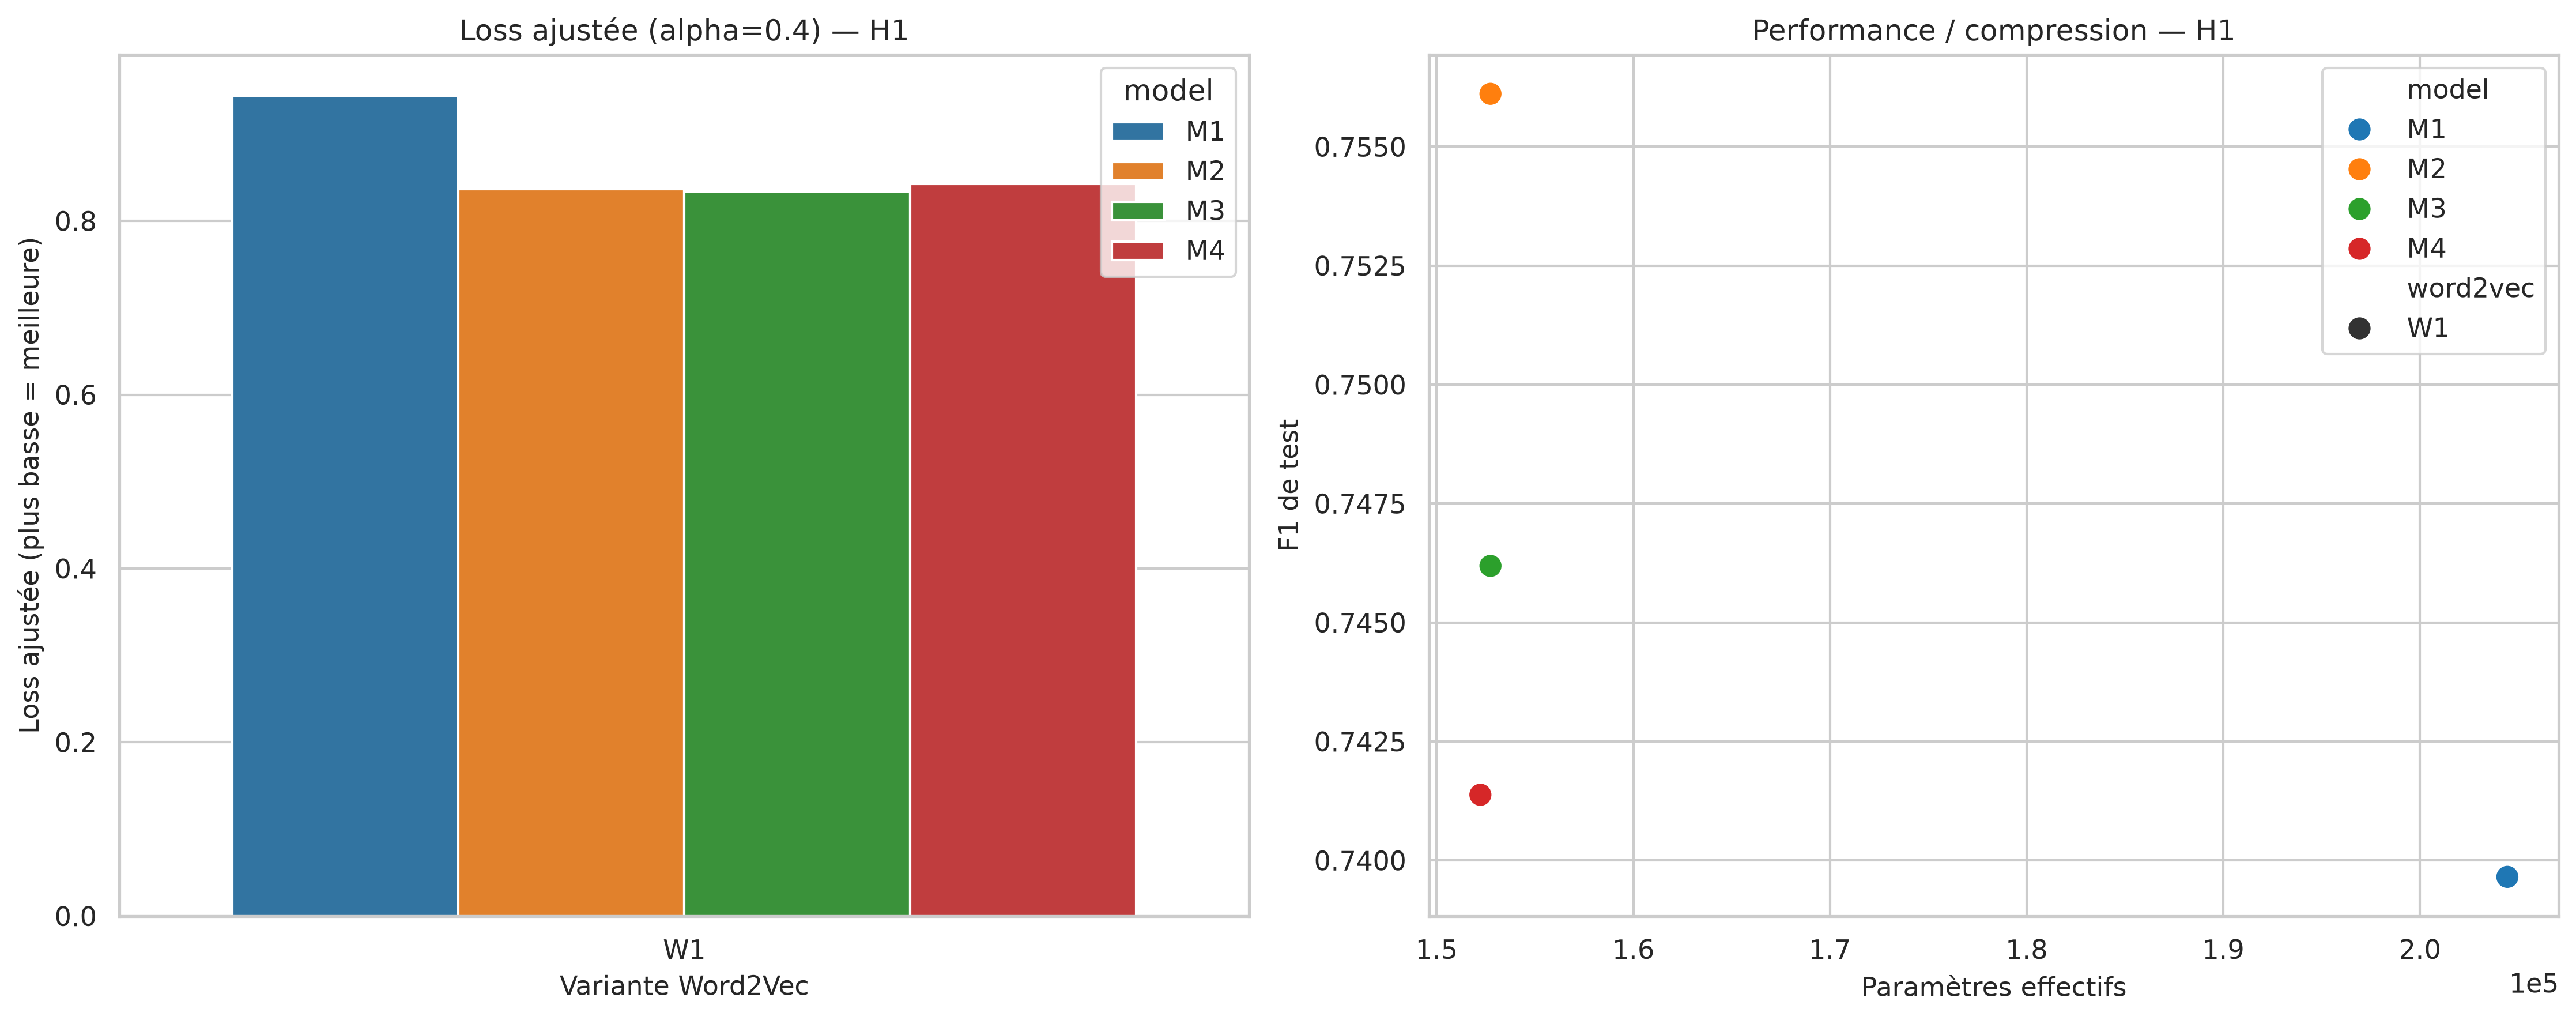
\includegraphics[width=0.94\textwidth]{../figures/experimentales/adjusted_loss_benchmark_H1.png}
    \par\smallskip\small (a) H1.\par\medskip
    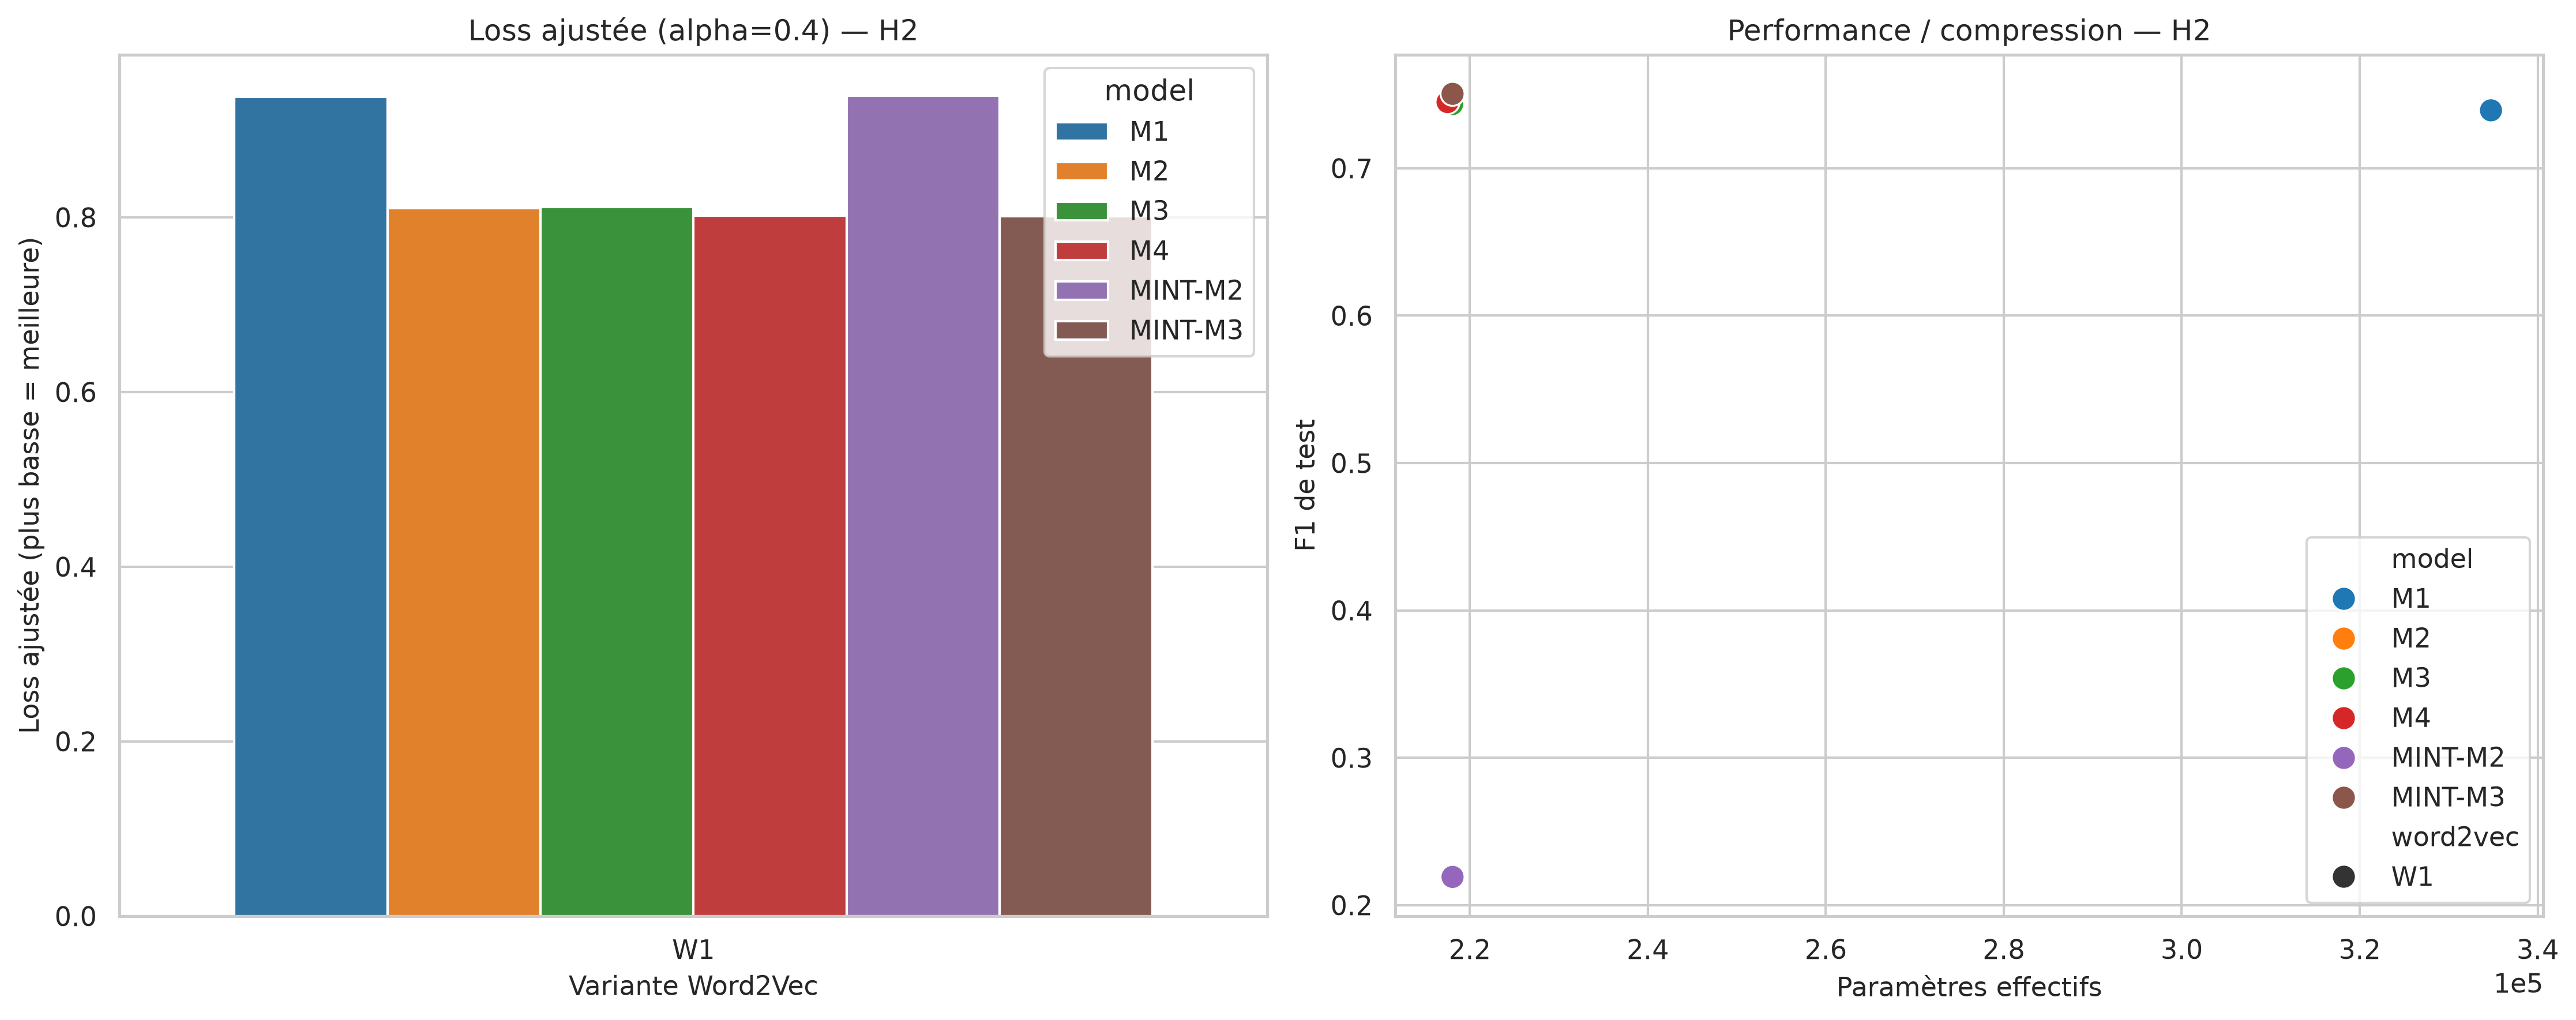
\includegraphics[width=0.94\textwidth]{../figures/experimentales/adjusted_loss_benchmark_H2.png}
    \par\smallskip\small (b) H2.
    \caption{Loss ajustée (à gauche) et F1 brut en fonction des paramètres
    effectifs (à droite). L'ajustement repose sur le nombre de paramètres
    effectifs du pipeline, backbone compris :
    $\mathcal{L}_{\text{ajustée}}=\mathcal{L}_{\mathrm{test}}+
    0{,}4\,P_{\mathrm{pipeline}}^{\mathrm{eff}}/
    P_{\mathrm{pipeline}}^{\mathrm{M1}}$. Il ne dépend pas du nombre de MAC ;
    une loss ajustée plus faible est meilleure.}
    \label{fig:resultats_loss_ajustee}
\end{figure}

Avec $\alpha=0{,}4$, H1/M3 obtient la plus faible loss ajustée
($0{,}8342$), devant M2 ($0{,}8367$) et M4 ($0{,}8428$). Pour H2, MINT-M3
($0{,}8015$) et M4 ($0{,}8018$) sont pratiquement à égalité. M1 conserve la
meilleure loss brute de H2, mais sa pénalisation de complexité porte sa loss
ajustée à $0{,}9381$. MINT-M2 reste mauvais ($0{,}9392$) : réduire le nombre
de poids ne compense pas une perte prédictive aussi importante.

\begin{figure}[!htbp]
    \centering
    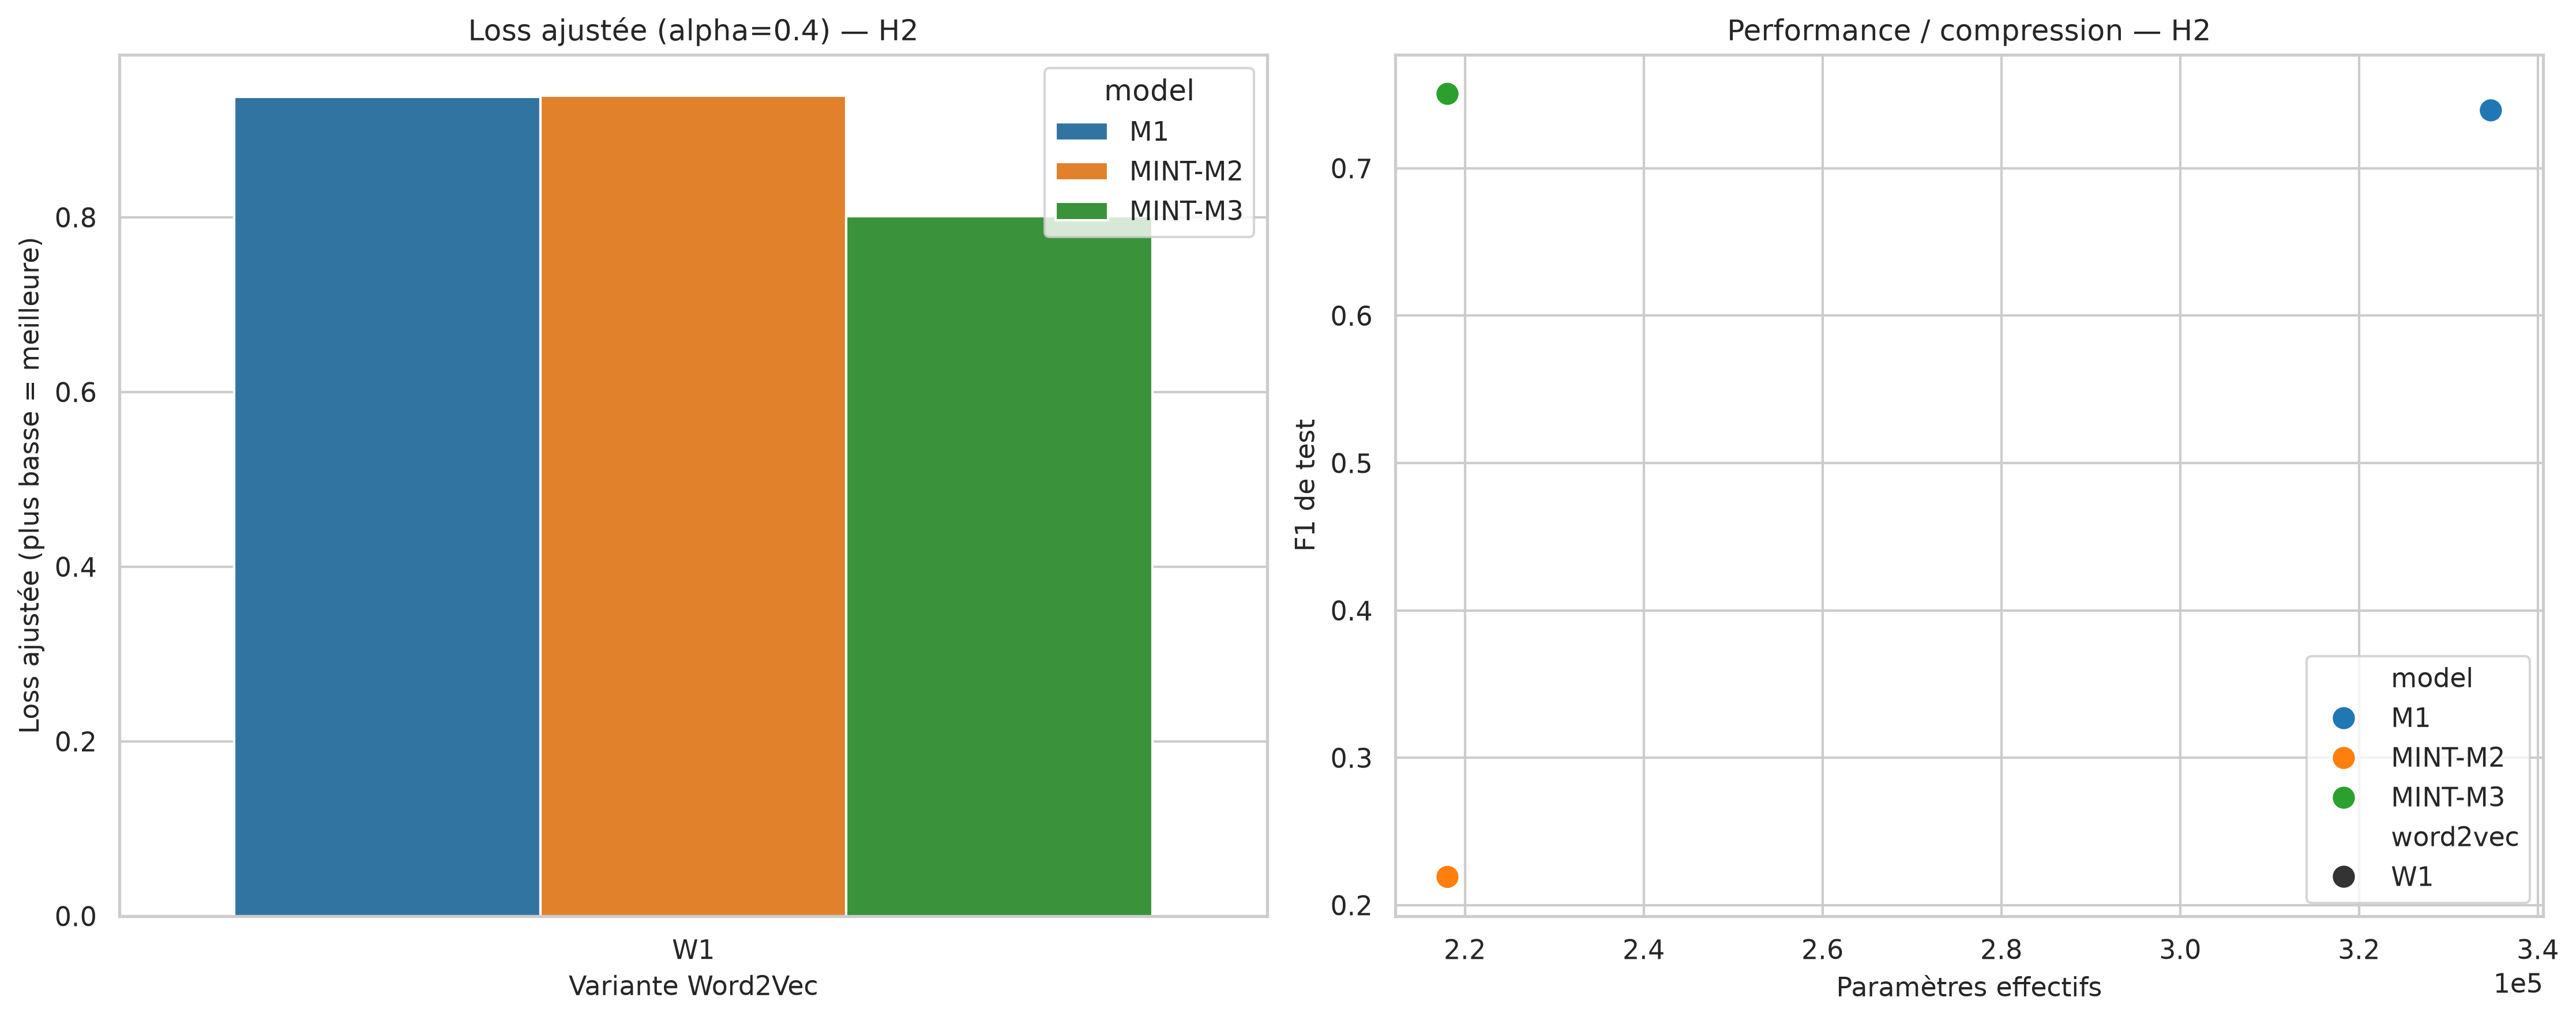
\includegraphics[width=0.9\textwidth]{../figures/experimentales/adjusted_loss_mint_W1_H2.png}
    \caption{Vue ciblée de la loss ajustée pour M1, MINT-M2 et MINT-M3.
    L'ajustement pénalise le nombre de paramètres effectifs du pipeline,
    backbone compris, et non le nombre de MAC. Cette figure isole l'effet du
    réentraînement à masque MINT constant : M2 et M3 ont le même nombre de
    paramètres, donc toute leur différence provient de la qualité retrouvée
    pendant la cicatrisation.}
    \label{fig:resultats_loss_ajustee_mint}
\end{figure}

\begin{figure}[!htbp]
    \centering
    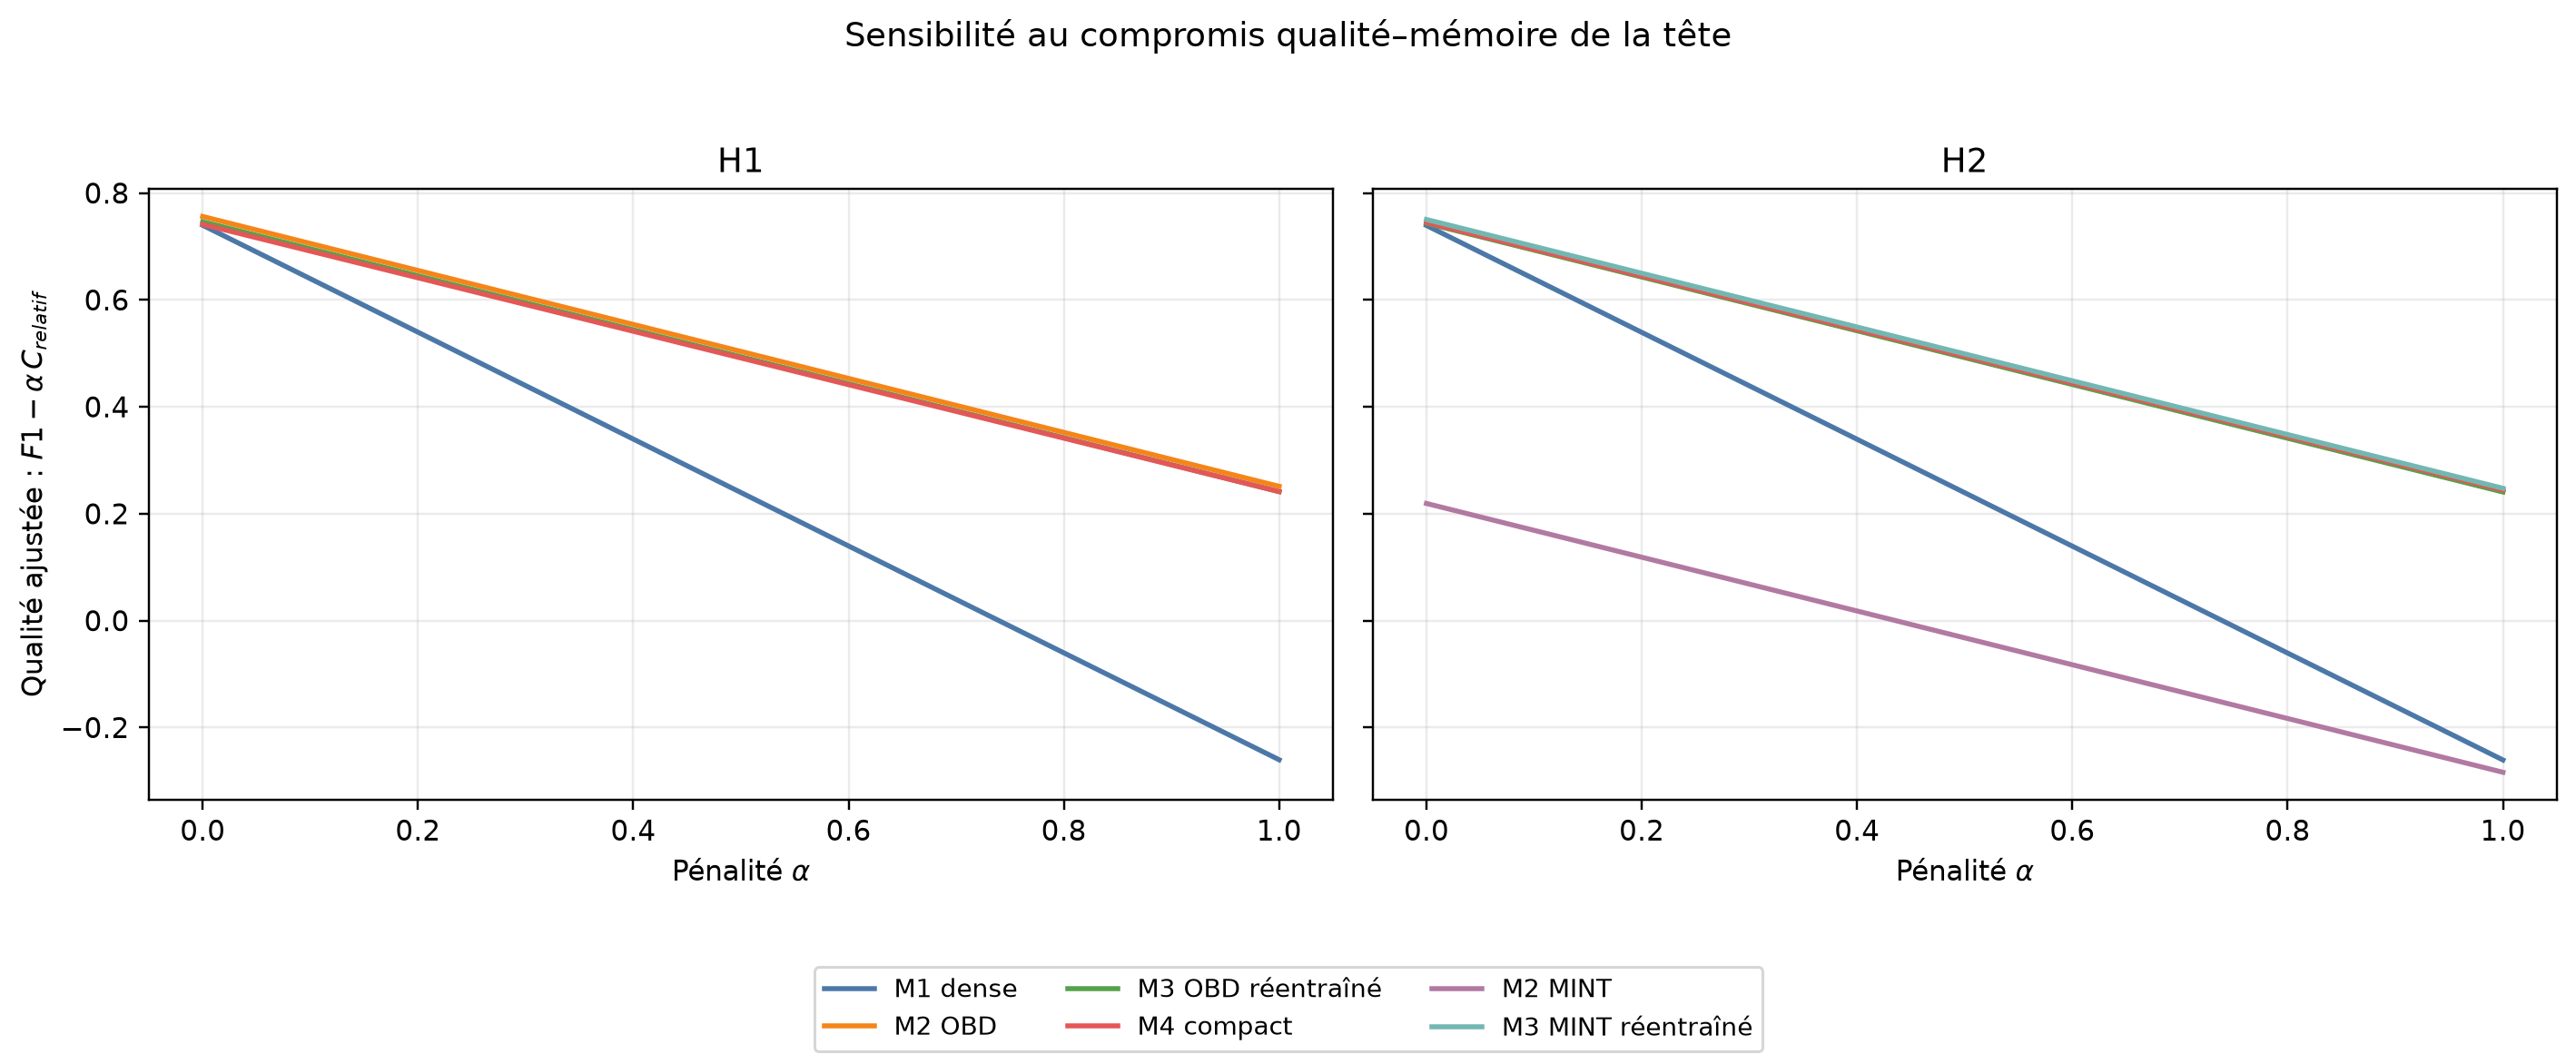
\includegraphics[width=0.94\textwidth]{../figures/experimentales/qualite_ajustee_memoire_tete.png}
    \caption{F1 ajusté en fonction de $\alpha$ à partir du nombre de paramètres
    effectifs de la tête :
    $F1_{\text{ajusté}}=F1-\alpha\,
    P_H^{\mathrm{eff}}/P_H^{\mathrm{M1}}$. L'ajustement porte donc sur les
    paramètres, et non sur les MAC. Sur $[0,1]$, H1/M2 et H2/MINT-M3 restent
    les meilleures solutions.}
    \label{fig:resultats_f1_ajuste_memoire_tete}
\end{figure}

\begin{figure}[!htbp]
    \centering
    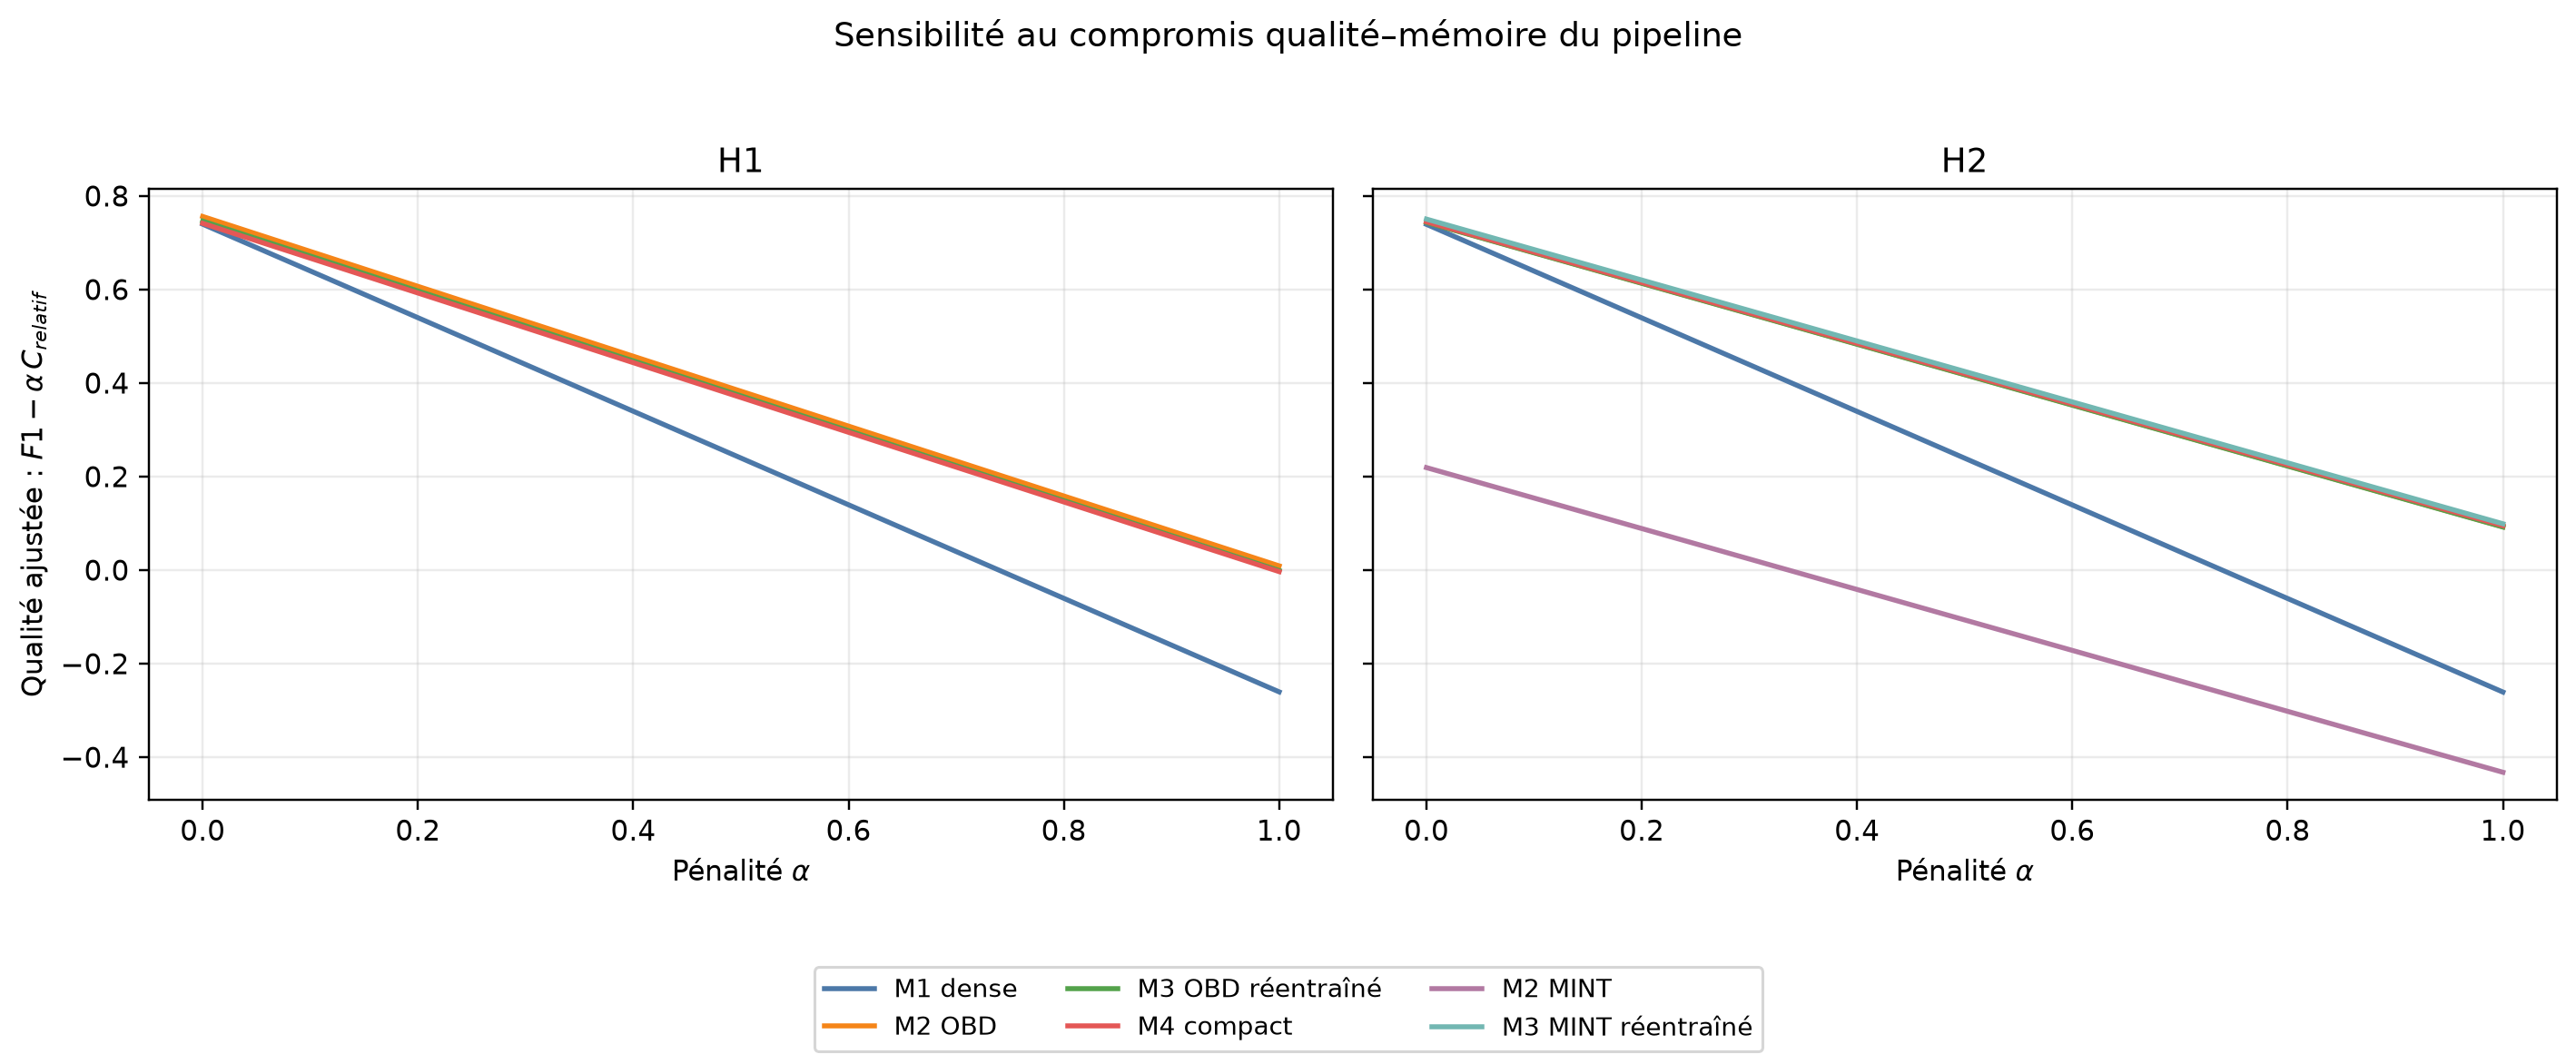
\includegraphics[width=0.94\textwidth]{../figures/experimentales/qualite_ajustee_memoire_pipeline.png}
    \caption{F1 ajusté à partir du nombre de paramètres effectifs du pipeline
    complet : $F1_{\text{ajusté}}=F1-\alpha\,
    P_{\mathrm{pipeline}}^{\mathrm{eff}}/
    P_{\mathrm{pipeline}}^{\mathrm{M1}}$. Cet ajustement porte sur les
    paramètres, et non sur les MAC. Le coût fixe de W1 réduit la pente par
    rapport à la vue tête seule.}
    \label{fig:resultats_f1_ajuste_memoire_pipeline}
\end{figure}

La \autoref{fig:resultats_f1_ajuste_memoire_tete} et la
\autoref{fig:resultats_f1_ajuste_memoire_pipeline} ajustent le F1 à partir du
nombre de paramètres. La \autoref{fig:resultats_f1_ajuste_calcul} utilise au
contraire le coût de calcul : la pénalité est le ratio entre le nombre de MAC
effectives idéales de la tête considérée et celui de la tête dense M1. Cette
quantité représente des opérations théoriquement évitables ; elle ne correspond
pas à la latence mesurée, puisque les couches PyTorch restent denses.

\begin{figure}[!htbp]
    \centering
    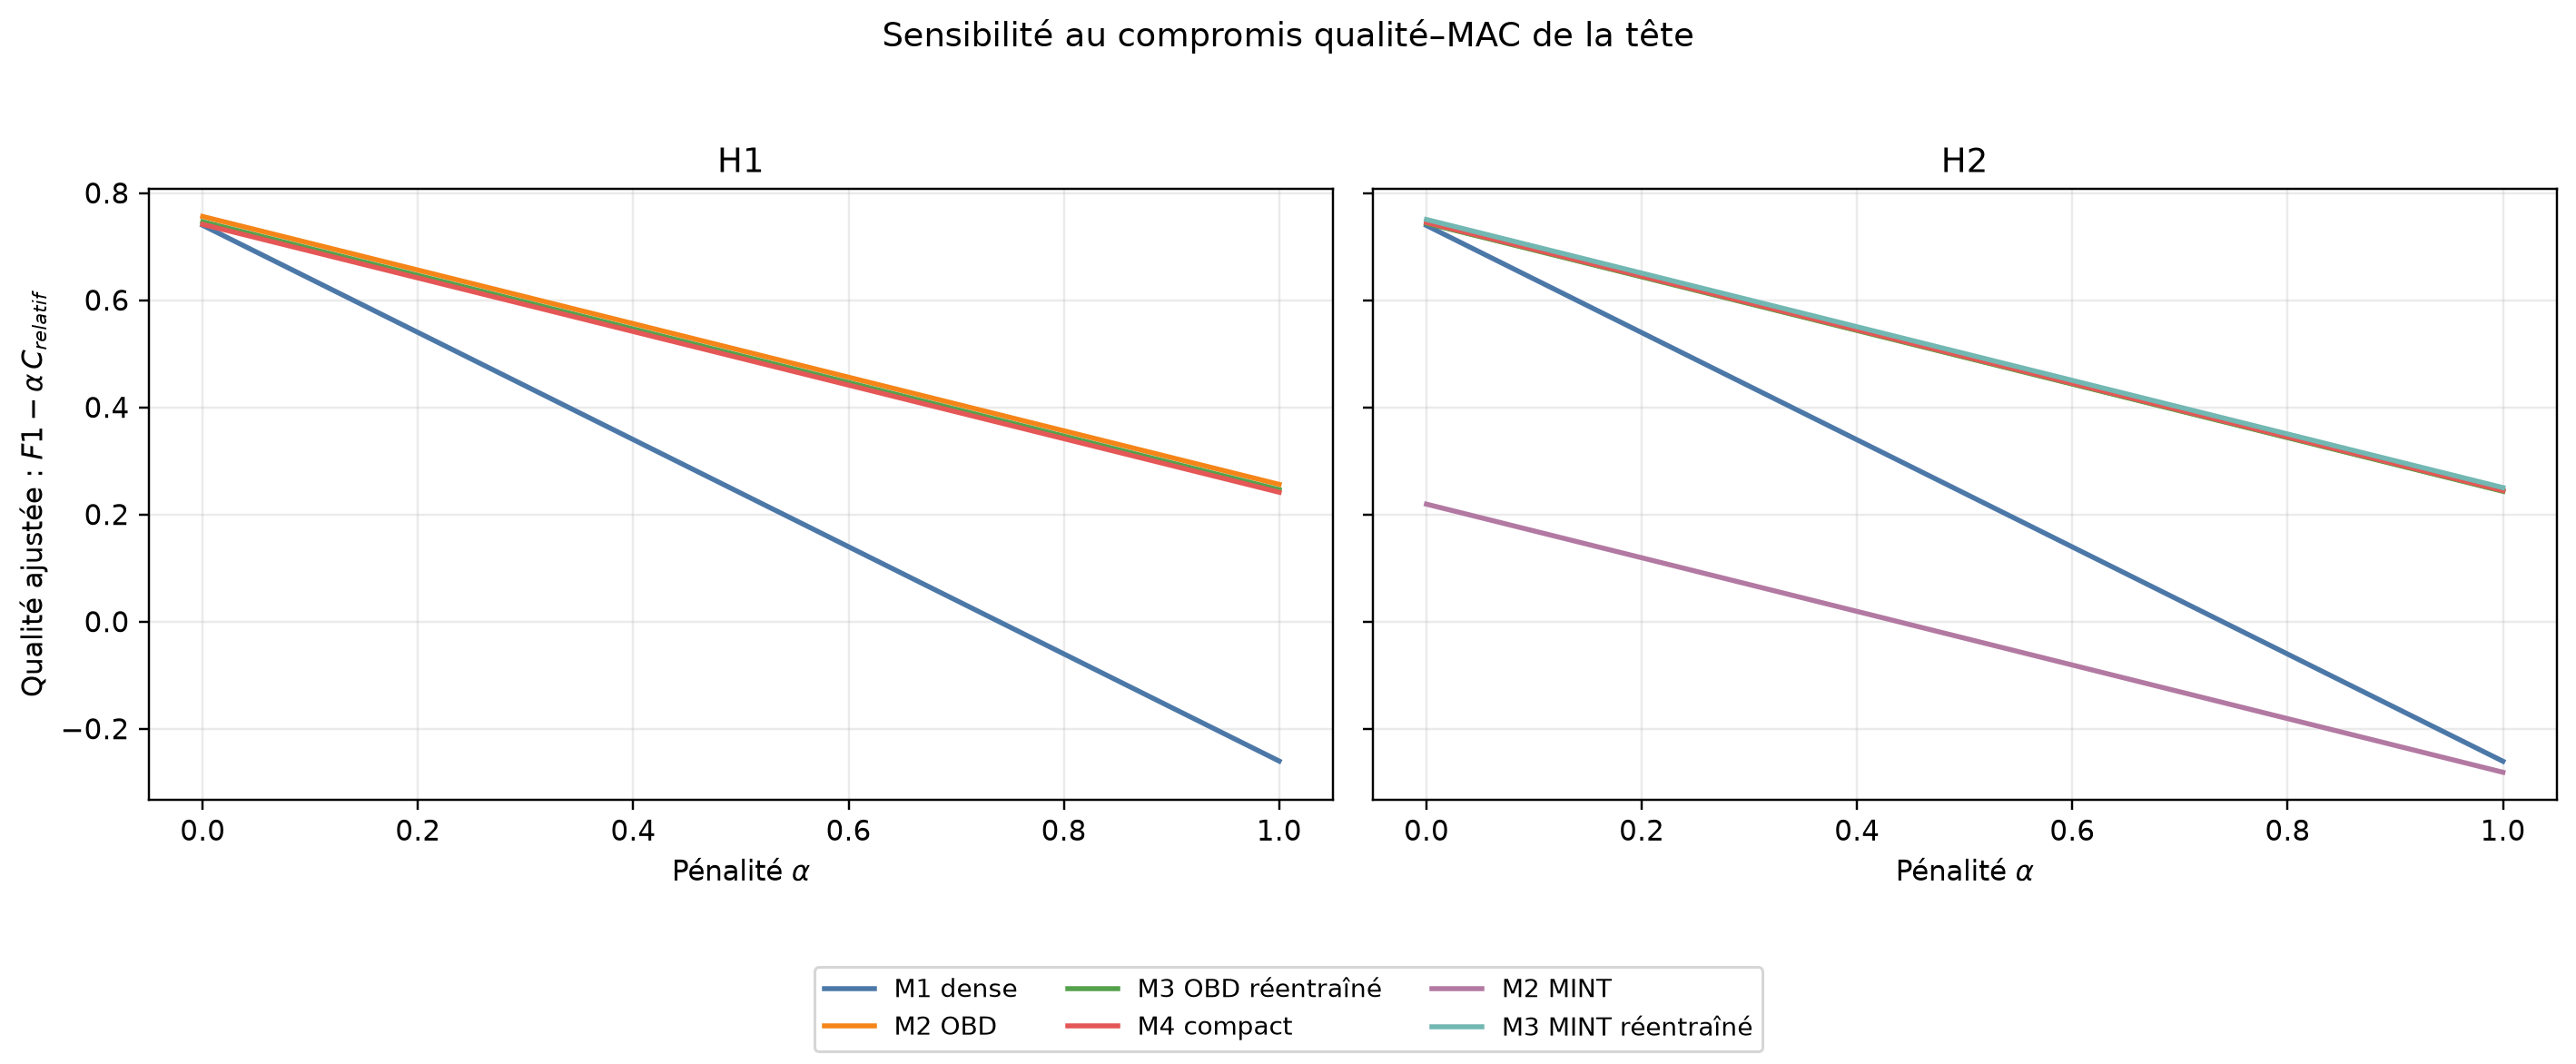
\includegraphics[width=0.94\textwidth]{../figures/experimentales/qualite_ajustee_calcul_tete.png}
    \caption{F1 ajusté à partir du nombre d'opérations de la tête, exprimé en
    MAC effectives idéales : $F1_{\text{ajusté}}=F1-\alpha\,
    C_H^{\mathrm{eff}}/C_H^{\mathrm{M1}}$. Cet ajustement porte donc sur les
    opérations, et non sur le nombre de paramètres. Les courbes restent proches
    de celles de la mémoire tête seule, car chaque poids actif d'une couche
    linéaire correspond ici à une MAC potentielle.}
    \label{fig:resultats_f1_ajuste_calcul}
\end{figure}

\paragraph{Synthèse selon l'accuracy ajustée.}
Pour compléter les courbes de F1, le tableau~\ref{tab:accuracy_ajustee} applique le
même principe à l'accuracy de test avec $\alpha=0{,}4$. Les trois scores sont
respectivement pénalisés par le ratio de paramètres effectifs de la tête, le
ratio de paramètres effectifs du pipeline et le ratio de MAC effectives idéales
de la tête, chaque ratio étant normalisé par M1. Ces valeurs sont des critères
de classement, et non des pourcentages d'accuracy.

\begin{table}[!htbp]
    \centering
    \resizebox{\textwidth}{!}{%
    \begin{tabular}{|l|l|r|r|r|r|}
        \hline
        Tête & Modèle & Accuracy brute &
        $\mathrm{Acc}_{\alpha}^{P_H}$ &
        $\mathrm{Acc}_{\alpha}^{P_{\mathrm{pipeline}}}$ &
        $\mathrm{Acc}_{\alpha}^{\mathrm{MAC}_H}$ \\ \hline
        H1 & M1     & $72{,}92\,\%$ & $0{,}3292$ & $0{,}3292$ & $0{,}3292$ \\ \hline
        H1 & M2 OBD & $73{,}20\,\%$ & $0{,}5300$ & $0{,}4332$ & $0{,}5320$ \\ \hline
        H1 & M3 OBD & $73{,}57\,\%$ & $\mathbf{0{,}5337}$ & $\mathbf{0{,}4368}$ & $\mathbf{0{,}5357}$ \\ \hline
        H1 & M4     & $72{,}53\,\%$ & $0{,}5253$ & $0{,}4275$ & $0{,}5253$ \\ \hline
        H2 & M1     & $73{,}26\,\%$ & $0{,}3326$ & $0{,}3326$ & $0{,}3326$ \\ \hline
        H2 & M2 OBD & $72{,}07\,\%$ & $0{,}5196$ & $0{,}4602$ & $0{,}5206$ \\ \hline
        H2 & M3 OBD & $73{,}02\,\%$ & $\mathbf{0{,}5291}$ & $\mathbf{0{,}4696}$ & $\mathbf{0{,}5300}$ \\ \hline
        H2 & M4     & $72{,}92\,\%$ & $0{,}5290$ & $0{,}4693$ & $0{,}5291$ \\ \hline
        H2 & MINT-M2 & $53{,}02\,\%$ & $0{,}3291$ & $0{,}2697$ & $0{,}3300$ \\ \hline
        H2 & MINT-M3 & $72{,}68\,\%$ & $0{,}5256$ & $0{,}4662$ & $0{,}5266$ \\ \hline
    \end{tabular}}
    \caption{Accuracy ajustée avec $\alpha=0{,}4$. Les colonnes pénalisent,
    de gauche à droite, le nombre de paramètres effectifs de la tête, le nombre
    de paramètres effectifs du pipeline complet et le nombre de MAC effectives
    idéales de la tête. Les valeurs en gras indiquent le meilleur modèle de
    chaque tête pour le critère considéré.}
    \label{tab:accuracy_ajustee}
\end{table}

OBD-M3 maximise les trois formes d'accuracy ajustée pour H1 comme pour H2. Sur
H2, l'écart avec M4 reste toutefois inférieur à $0{,}001$ pour les trois
critères : ce classement très fin ne doit donc pas être interprété comme un
avantage statistiquement établi avec une seule graine.

Pour les courbes de F1, l'analyse de sensibilité ne fait pas apparaître de
changement de vainqueur sur $\alpha\in[0,1]$. Ce constat ne signifie pas que le choix de $\alpha$ est sans
importance : il résulte du fait que les variantes réduites ont presque toutes
la même cible de capacité. L'intérêt principal de ces figures est alors de
montrer à quelle vitesse M1, plus coûteux, est dominé lorsque la compression
reçoit un poids croissant.

\subsection{Coût hors ligne du scoring}
\label{ssec:resultats_cout_scoring}

\begin{figure}[!htbp]
    \centering
    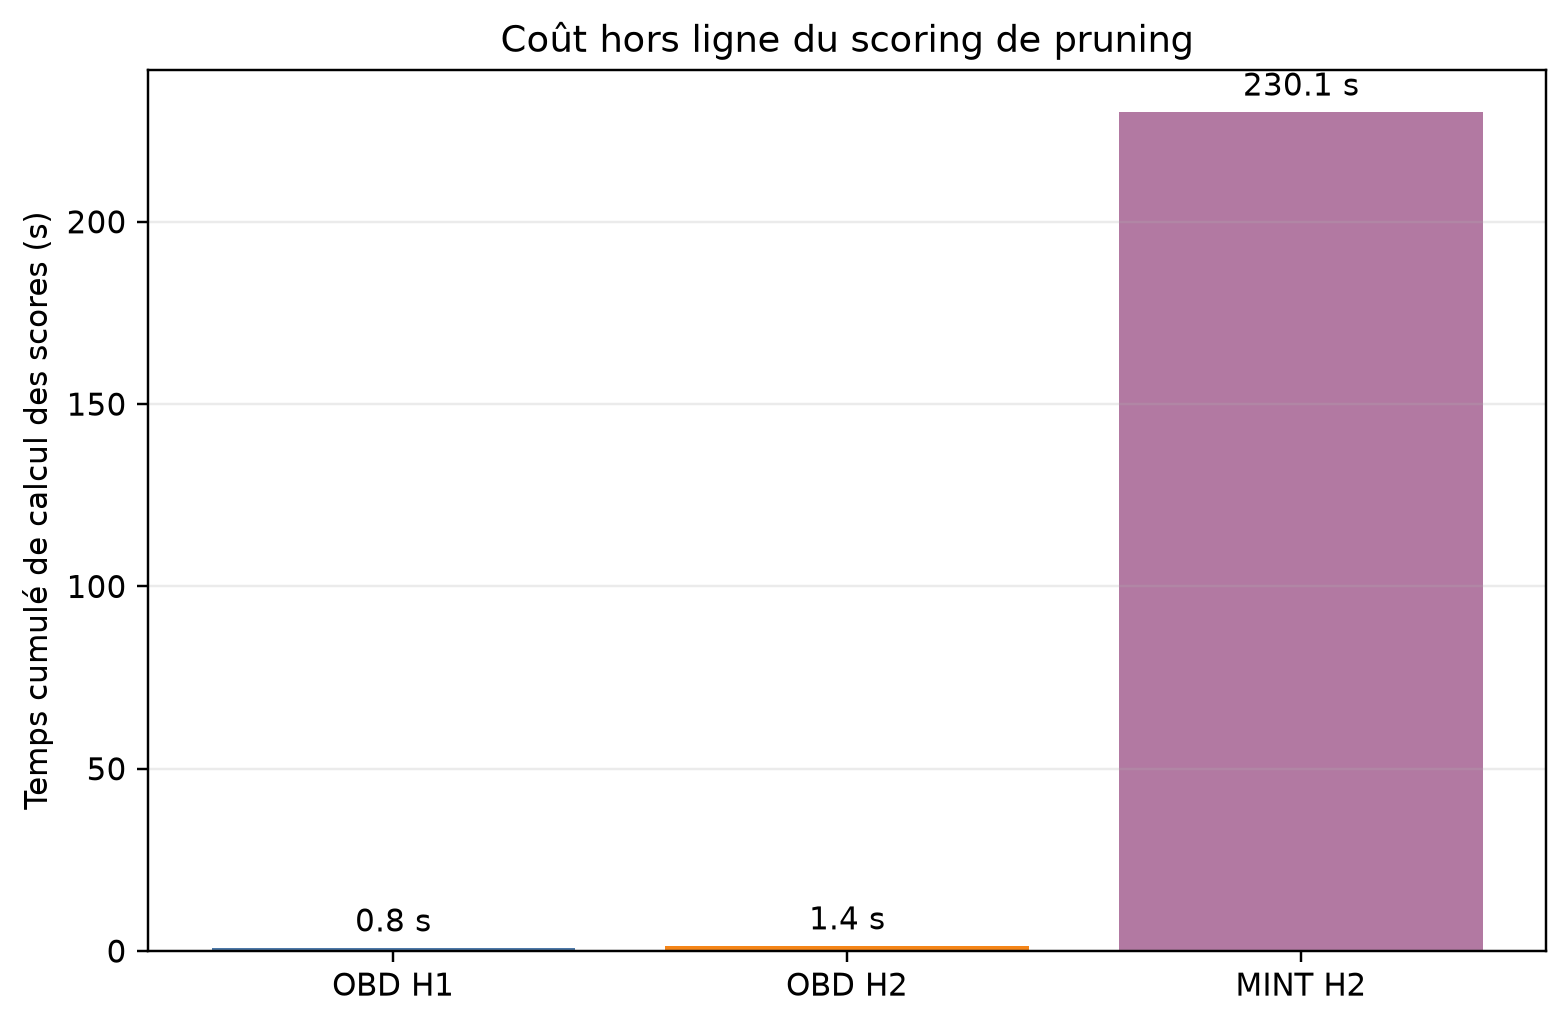
\includegraphics[width=0.78\textwidth]{../figures/experimentales/cout_scoring_pruning.png}
    \caption{Temps cumulé de calcul des scores. OBD inclut tous les tours de
    scoring itératif ; MINT inclut les $12\,296$ estimations GMI de ses trois
    couches, mais pas le réentraînement commun aux comparaisons de qualité.}
    \label{fig:resultats_cout_scoring}
\end{figure}

OBD demande $0{,}85$ seconde pour H1 et $1{,}41$ seconde pour H2. MINT demande
$230{,}1$ secondes sur H2, soit environ 163 fois le temps de scoring OBD de la
même tête. La première couche concentre $186{,}2$ secondes et la deuxième
$43{,}7$ secondes ; la sortie ne demande que $0{,}15$ seconde. Ce déséquilibre
s'explique par le nombre d'unités aval et donc de blocs à scorer. Dans cette
implémentation, le meilleur F1 de MINT-M3 s'accompagne ainsi d'un coût hors
ligne très supérieur.

\subsection{Gains idéaux et gains réellement observés}
\label{ssec:resultats_gains_reels}

Les mesures de latence sont effectuées sur CPU AMD Ryzen AI 9 365, sans CUDA,
avec PyTorch configuré sur 10 threads. Elles utilisent $2\,048$ textes de test
déjà tokenisés, des batches de 512, deux passages d'échauffement et la médiane
de sept répétitions. Le temps par texte est donc un temps \emph{amorti dans un
batch}, et non la latence d'une requête isolée. Le temps du pipeline additionne
l'agrégation des embeddings et la tête ; la tokenisation est exclue. La taille
mesurée est celle d'un artefact d'inférence dense contenant la table d'entrée
W1 et l'état du classifieur, sans table CBOW de sortie ni masque auxiliaire.

\begin{table}[!htbp]
    \centering
    \begin{tabular}{|l|l|r|r|r|}
        \hline
        Tête & Modèle & Tête ($\mu$s/texte) & Pipeline ($\mu$s/texte) & Artefact (KiB) \\ \hline
        H1 & M1 & $3{,}350$ & $16{,}432$ & $801{,}0$ \\ \hline
        H1 & M2 OBD & $3{,}195$ & $16{,}277$ & $801{,}0$ \\ \hline
        H1 & M3 OBD & $3{,}197$ & $16{,}280$ & $801{,}0$ \\ \hline
        H1 & M4 & $1{,}813$ & $14{,}896$ & $597{,}0$ \\ \hline
        H2 & M1 & $5{,}701$ & $18{,}784$ & $1\,310{,}4$ \\ \hline
        H2 & M2 OBD & $5{,}710$ & $18{,}792$ & $1\,310{,}4$ \\ \hline
        H2 & M3 OBD & $5{,}707$ & $18{,}790$ & $1\,310{,}4$ \\ \hline
        H2 & M4 & $3{,}291$ & $16{,}374$ & $852{,}4$ \\ \hline
        H2 & MINT-M2 & $5{,}704$ & $18{,}786$ & $1\,310{,}4$ \\ \hline
        H2 & MINT-M3 & $5{,}707$ & $18{,}790$ & $1\,310{,}4$ \\ \hline
    \end{tabular}
    \caption{Mesures physiques du format dense actuel. Les faibles différences
    entre variantes de même architecture sont du même ordre que la variabilité
    d'un microbenchmark et ne doivent pas être interprétées comme une
    accélération due aux zéros.}
    \label{tab:resultats_runtime}
\end{table}

\begin{figure}[!htbp]
    \centering
    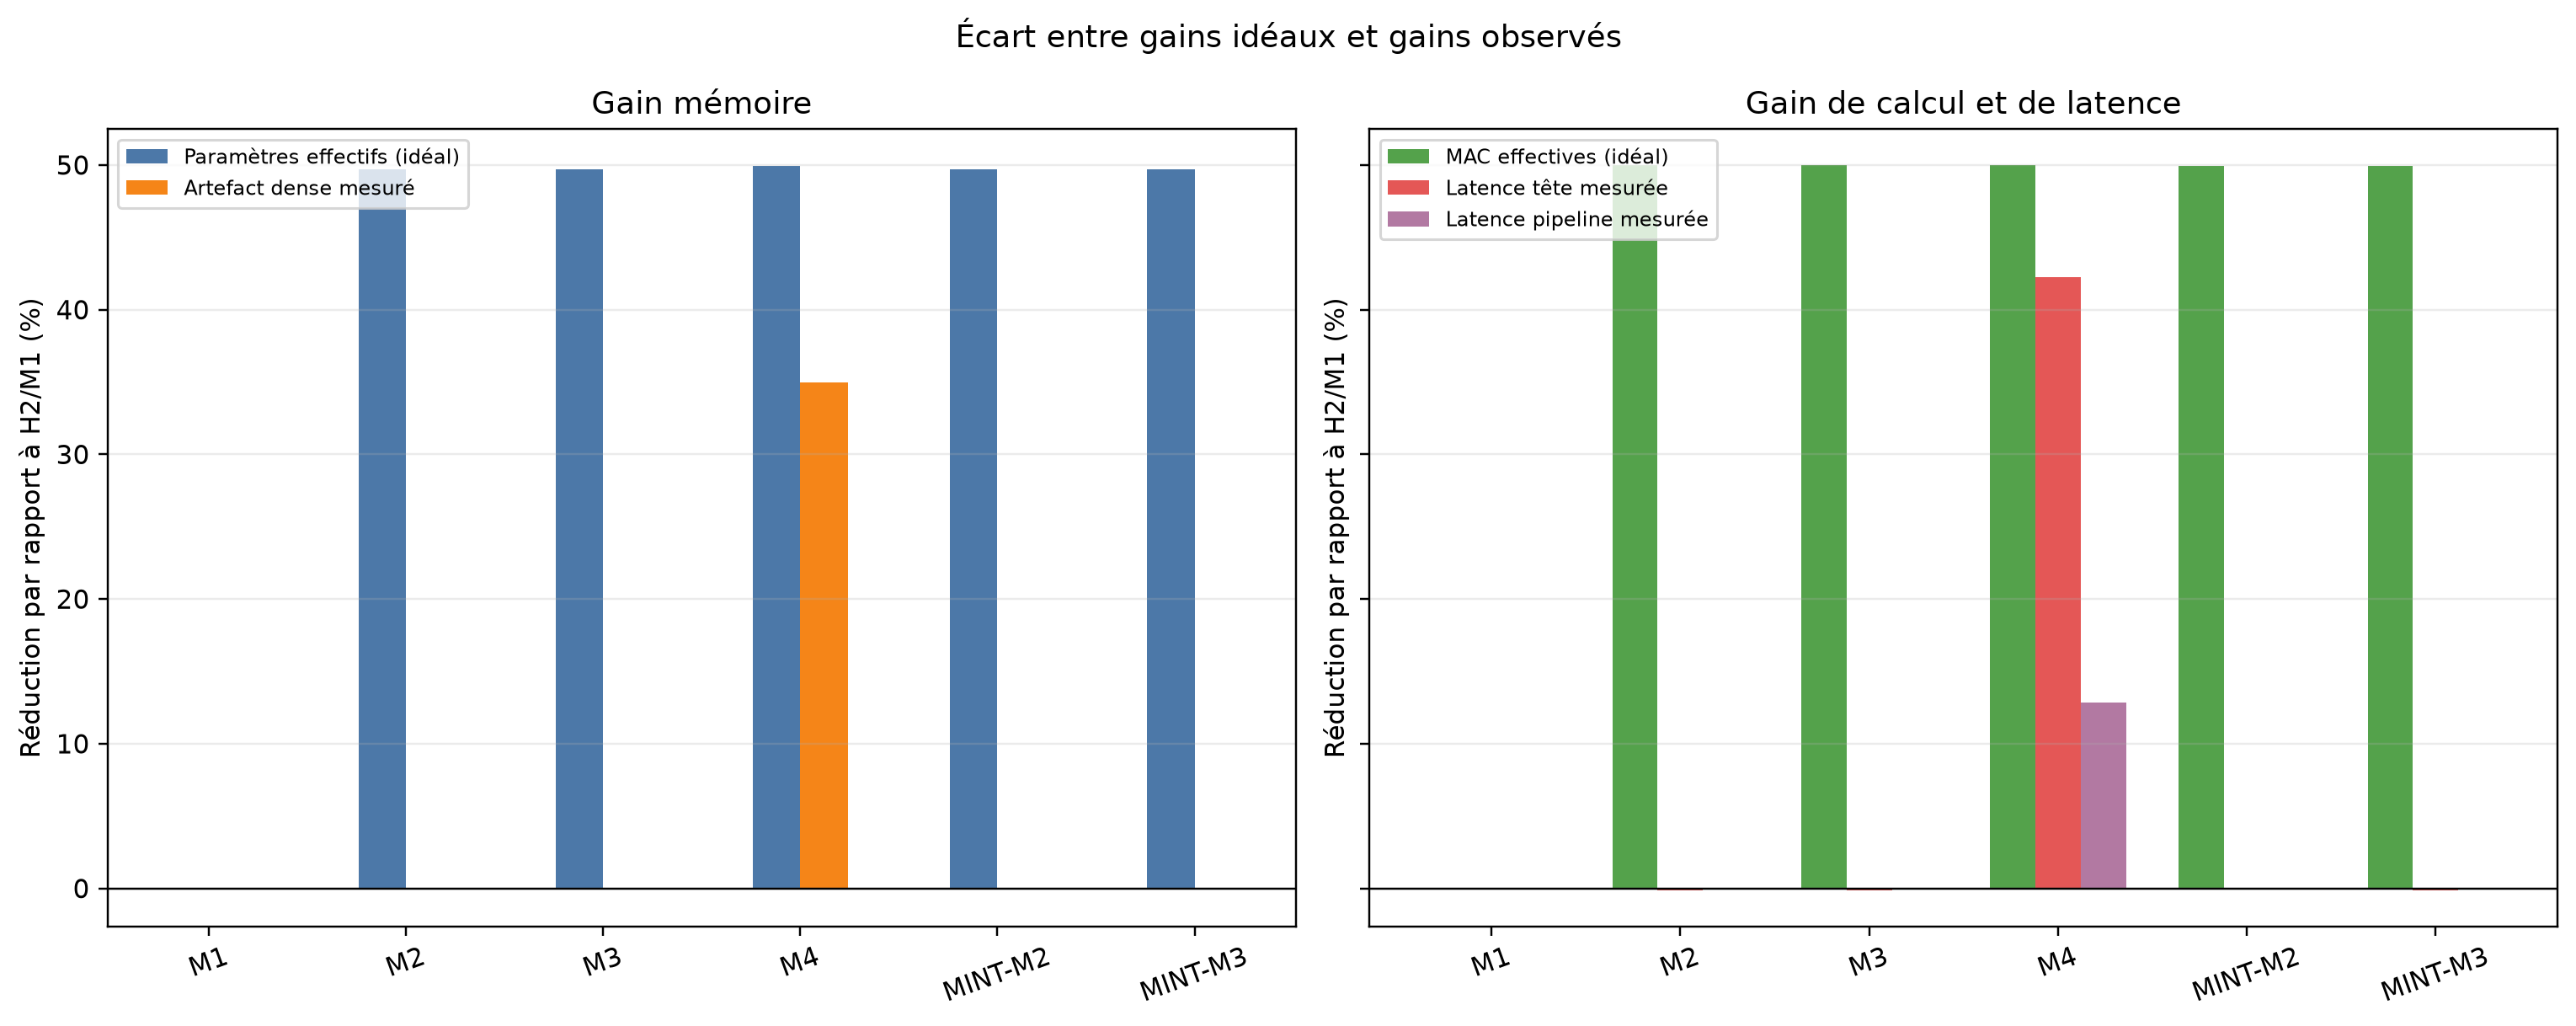
\includegraphics[width=0.96\textwidth]{../figures/experimentales/gain_theorique_vs_reel.png}
    \caption{Réductions idéales et observées pour H2, relativement à M1.
    Les masques OBD et MINT divisent par deux les paramètres et MAC effectifs
    théoriques, mais les tenseurs denses conservent leur taille et leur temps
    d'exécution. Seule M4 modifie physiquement les dimensions.}
    \label{fig:resultats_gain_theorique_reel}
\end{figure}

Le résultat central de la \autoref{fig:resultats_gain_theorique_reel} est
l'absence de gain réel pour les masques. OBD-M2, OBD-M3, MINT-M2 et MINT-M3
occupent exactement la même taille sérialisée que H2/M1 et leurs temps diffèrent
de moins de $0{,}2\,\%$. PyTorch exécute toujours les matrices complètes. M4
réduit au contraire la taille de l'artefact H2 de $34{,}95\,\%$, la latence de
la tête de $42{,}27\,\%$ et celle du pipeline de $12{,}83\,\%$. Pour H1, M4
réduit respectivement ces quantités de $25{,}47\,\%$, $45{,}87\,\%$ et
$9{,}35\,\%$.

Le backbone explique l'écart entre la tête et le pipeline : son agrégation
demande environ $13{,}08\,\mu$s par texte dans ce protocole, quel que soit le
classifieur. Une forte réduction du temps de la tête devient donc une réduction
plus modeste du temps bout en bout.

\subsection{Comparaison au pruning aléatoire}
\label{ssec:resultats_random}

Le pruning aléatoire est répété avec les cinq mêmes graines que les autres
méthodes. Il utilise aussi la même sparsité et le même calendrier qu'OBD. Le
tableau~\ref{tab:resultats_random} présente les résultats avant et après le
dernier réentraînement.

\begin{table}[!htbp]
    \centering
    \resizebox{\textwidth}{!}{%
    \begin{tabular}{|l|l|c|c|c|c|}
        \hline
        Tête & Modèle & Loss & Accuracy & F1 & ROC-AUC \\ \hline
        H1 & M1 & $0{,}5400\pm0{,}0044$ & $73{,}15\pm0{,}39\,\%$ & $0{,}7456\pm0{,}0048$ & $0{,}8045\pm0{,}0040$ \\ \hline
        H1 & RAND-M2 & $0{,}5487\pm0{,}0030$ & $72{,}00\pm0{,}40\,\%$ & $0{,}7308\pm0{,}0108$ & $0{,}7971\pm0{,}0032$ \\ \hline
        H1 & RAND-M3 & $0{,}5440\pm0{,}0034$ & $72{,}48\pm0{,}31\,\%$ & $0{,}7335\pm0{,}0057$ & $0{,}8006\pm0{,}0039$ \\ \hline
        H2 & M1 & $0{,}5486\pm0{,}0063$ & $72{,}73\pm0{,}61\,\%$ & $0{,}7321\pm0{,}0082$ & $0{,}8009\pm0{,}0035$ \\ \hline
        H2 & RAND-M2 & $0{,}5872\pm0{,}0178$ & $69{,}38\pm3{,}19\,\%$ & $0{,}6467\pm0{,}0743$ & $0{,}7880\pm0{,}0066$ \\ \hline
        H2 & RAND-M3 & $0{,}5433\pm0{,}0046$ & $72{,}70\pm0{,}45\,\%$ & $0{,}7323\pm0{,}0139$ & $0{,}8020\pm0{,}0032$ \\ \hline
    \end{tabular}}
    \caption{Métriques de test du témoin aléatoire sur cinq graines. Chaque
    valeur est la moyenne $\pm$ l'écart-type empirique. RAND-M2 et RAND-M3 ont
    exactement la sparsité et le nombre de poids actifs de leurs homologues
    OBD.}
    \label{tab:resultats_random}
\end{table}

Sur H1, RAND-M3 obtient un F1 de $0{,}7335$, contre $0{,}7456$ pour M1 et
$0{,}7512$ pour OBD-M3. La comparaison graine par graine confirme l'écart entre
OBD-M3 et RAND-M3 : l'intervalle à $95\,\%$ ne contient pas zéro. Sur H1, OBD
choisit donc de meilleurs poids qu'un tirage au hasard.

Sur H2, le masque aléatoire fait d'abord fortement baisser le F1 : RAND-M2
obtient $0{,}6467$. Après le dernier réentraînement, RAND-M3 remonte à
$0{,}7323$, presque au même niveau que M1 ($0{,}7321$). OBD-M3 et MINT-M3 ont
des moyennes un peu plus élevées, mais les écarts avec RAND-M3 ne sont pas assez
clairs avec seulement cinq graines. Sur H2, le réentraînement semble donc plus
important que la manière de choisir le masque.

La comparaison avec OBD est directe, car OBD et RAND suivent le même protocole.
MINT utilise des blocs et un pruning en une seule passe ; ses résultats avant
réentraînement ne sont donc pas directement comparables à ceux de RAND-M2.

\subsection{Robustesse sur cinq graines}
\label{ssec:resultats_repetitions}

Le run de la graine 42 permet d'étudier les trajectoires, les distributions de
scores et les coûts avec un niveau de détail fin. Pour vérifier que son
classement ne dépend pas d'une initialisation particulière, le protocole de la
\autoref{ssec:methode_repetitions} répète ensuite les entraînements avec les
graines 42 à 46. Le backbone W1, les vecteurs et les trois partitions de données
restent fixes. Le tableau~\ref{tab:resultats_repetes} rapporte donc une
variabilité algorithmique, et non une variabilité due au choix du corpus ou du
jeu de test.

\begin{table}[!htbp]
    \centering
    \resizebox{\textwidth}{!}{%
    \begin{tabular}{|l|l|c|c|c|c|c|}
        \hline
        Tête & Modèle & Loss & Accuracy & F1 & $s_{F1}^{2}$ & ROC-AUC \\ \hline
        H1 & M1 & $0{,}5400\pm0{,}0044$ & $73{,}15\pm0{,}39\,\%$ & $0{,}7456\pm0{,}0048$ & $2{,}30\times10^{-5}$ & $0{,}8045\pm0{,}0040$ \\ \hline
        H1 & M2 OBD & $\mathbf{0{,}5328\pm0{,}0023}$ & $\mathbf{73{,}47\pm0{,}15\,\%}$ & $0{,}7491\pm0{,}0032$ & $1{,}04\times10^{-5}$ & $\mathbf{0{,}8115\pm0{,}0023}$ \\ \hline
        H1 & M3 OBD & $0{,}5337\pm0{,}0019$ & $73{,}46\pm0{,}23\,\%$ & $\mathbf{0{,}7512\pm0{,}0048}$ & $2{,}32\times10^{-5}$ & $0{,}8108\pm0{,}0020$ \\ \hline
        H1 & M4 & $0{,}5411\pm0{,}0034$ & $72{,}89\pm0{,}51\,\%$ & $0{,}7463\pm0{,}0050$ & $2{,}49\times10^{-5}$ & $0{,}8037\pm0{,}0034$ \\ \hline
        H2 & M1 & $0{,}5486\pm0{,}0063$ & $72{,}73\pm0{,}61\,\%$ & $0{,}7321\pm0{,}0082$ & $6{,}78\times10^{-5}$ & $0{,}8009\pm0{,}0035$ \\ \hline
        H2 & M2 OBD & $0{,}5632\pm0{,}0159$ & $72{,}75\pm0{,}39\,\%$ & $0{,}7325\pm0{,}0111$ & $1{,}23\times10^{-4}$ & $0{,}7982\pm0{,}0070$ \\ \hline
        H2 & M3 OBD & $0{,}5716\pm0{,}0172$ & $72{,}63\pm0{,}47\,\%$ & $0{,}7371\pm0{,}0068$ & $4{,}69\times10^{-5}$ & $0{,}7992\pm0{,}0078$ \\ \hline
        H2 & M4 & $0{,}5510\pm0{,}0096$ & $71{,}97\pm1{,}39\,\%$ & $0{,}7345\pm0{,}0100$ & $9{,}92\times10^{-5}$ & $0{,}7938\pm0{,}0114$ \\ \hline
        H2 & MINT-M2 & $0{,}6873\pm0{,}0187$ & $52{,}60\pm2{,}72\,\%$ & $0{,}2028\pm0{,}0938$ & $8{,}79\times10^{-3}$ & $0{,}7208\pm0{,}0149$ \\ \hline
        H2 & MINT-M3 & $\mathbf{0{,}5394\pm0{,}0019}$ & $\mathbf{72{,}89\pm0{,}56\,\%}$ & $\mathbf{0{,}7430\pm0{,}0101}$ & $1{,}03\times10^{-4}$ & $\mathbf{0{,}8045\pm0{,}0027}$ \\ \hline
    \end{tabular}}
    \caption{Métriques de test sur cinq graines. Chaque valeur est la moyenne
    $\pm$ l'écart-type empirique ; $s_{F1}^{2}$ donne explicitement la variance
    du F1. Les valeurs en gras sont les meilleures moyennes de chaque tête,
    sans préjuger de la portée statistique de leur écart. Les variances et les
    intervalles des autres métriques restent disponibles dans les artefacts.}
    \label{tab:resultats_repetes}
\end{table}

Le classement moyen des accuracies ajustées est donné dans le
tableau~\ref{tab:accuracy_ajustee_repetee}. Le passage de la graine unique aux
cinq répétitions remplace H1/OBD-M3 par H1/OBD-M2 et H2/OBD-M3 par H2/MINT-M3.
Ces inversions restent toutefois minuscules : l'intervalle apparié entre les
deux modèles de tête pour le score ajusté contient zéro dans chaque cas.

\begin{table}[!htbp]
    \centering
    \begin{tabular}{|l|l|r|r|r|}
        \hline
        Tête & Meilleur modèle moyen &
        $\mathrm{Acc}_{\alpha}^{P_H}$ &
        $\mathrm{Acc}_{\alpha}^{P_{\mathrm{pipeline}}}$ &
        $\mathrm{Acc}_{\alpha}^{\mathrm{MAC}_H}$ \\ \hline
        H1 & M2 OBD & $0{,}5327$ & $0{,}4359$ & $0{,}5347$ \\ \hline
        H2 & MINT-M3 & $0{,}5277$ & $0{,}4683$ & $0{,}5287$ \\ \hline
    \end{tabular}
    \caption{Meilleurs modèles selon l'accuracy ajustée moyenne sur cinq
    graines, avec $\alpha=0{,}4$. Les trois colonnes pénalisent respectivement
    les paramètres effectifs de la tête, ceux du pipeline et les MAC effectives
    idéales de la tête.}
    \label{tab:accuracy_ajustee_repetee}
\end{table}

\subsection{Réponses aux questions expérimentales et limites}
\label{ssec:resultats_reponses_limites}

Les six questions de la \autoref{ssec:probleme_questions} reçoivent les
réponses suivantes. OBD peut retirer environ la moitié des poids sans perte de
F1 sur le test ; MINT provoque en revanche une perte immédiate majeure. Le
réentraînement récupère entièrement cette perte pour MINT, mais n'améliore pas
systématiquement OBD. À coût effectif presque identique, H1/M2 et H2/MINT-M3
obtiennent les meilleurs F1. Les gains théoriques des masques ne se traduisent
pas en gains physiques dans le format dense ; M4 constitue la seule compression
immédiatement exploitable. Enfin, le scoring MINT est deux ordres de grandeur
plus lent que celui d'OBD dans cette configuration.

Le témoin aléatoire montre qu'OBD fait mieux sur H1. Sur H2, les cinq graines ne
suffisent pas pour montrer qu'OBD ou MINT fait mieux que RAND-M3.

Les répétitions tempèrent cependant le classement du run détaillé. Avec cinq
graines, aucun gain apparié de F1 ou d'accuracy des modèles informés par rapport
à M1 n'a un intervalle à $95\,\%$ excluant zéro. Le split
et W1 restent fixes : les intervalles mesurent uniquement la variabilité
algorithmique et leur faible effectif ne permet pas une comparaison
statistique définitive. Le batch OBD est toujours constitué des 256 premiers
exemples d'entraînement, tandis que chaque score MINT repose sur une seule
permutation. Enfin, les temps sont des microbenchmarks CPU amortis, sans mesure
d'énergie ni de pic mémoire. Ces limites n'invalident ni la proximité moyenne
des F1 après réentraînement, ni le constat structurel sur les
tenseurs denses, mais elles interdisent de transformer le classement fin des
méthodes en conclusion générale.
